\pdfoutput=1
%% MERIDIAN: arXiv review draft, generated from paper/meridian.tex.
%% Build: pdflatex meridian && bibtex meridian && pdflatex meridian && pdflatex meridian
%% (TinyTeX: export PATH="$HOME/Library/TinyTeX/bin/universal-darwin:$PATH")
\documentclass[sigconf,nonacm]{acmart}

\usepackage{CJKutf8}
\usepackage{tikz}
\usetikzlibrary{arrows.meta,positioning,fit,calc,shapes.geometric}
\usepackage{subcaption}
\usepackage{booktabs}
\usepackage{multirow}
\usepackage{enumitem}
\usepackage{balance}
\setlength{\emergencystretch}{2em}
\raggedbottom

% Chinese in a Latin paper: Arphic Song for running text, Arphic Kai for quoted verse.
\pdfmapfile{=gbsnu.map}
\pdfmapfile{=gkaiu.map}
\newcommand{\zh}[1]{\begingroup\normalfont\begin{CJK*}{UTF8}{gbsn}#1\end{CJK*}\endgroup}
\newcommand{\kai}[1]{\begingroup\normalfont\begin{CJK*}{UTF8}{gkai}#1\end{CJK*}\endgroup}

% The town's palette, used in the diagrams.
\definecolor{navy}{HTML}{0B2036}
\definecolor{gold}{HTML}{D3A557}
\definecolor{cream}{HTML}{F6EFE2}
\definecolor{rose}{HTML}{C74B5F}
\definecolor{meadow}{HTML}{5F9E5A}
\definecolor{sky}{HTML}{3F7FB3}
\definecolor{merred}{HTML}{D7102F}

% A heart drawn in TikZ, so it prints in any PDF viewer (no emoji font needed).
\newsavebox{\heartbox}
\sbox{\heartbox}{\tikz[baseline=-0.32em,x=1.5em,y=1.5em]{\fill[merred]
  (0,-0.42) .. controls (-0.58,0.02) and (-0.56,0.5) .. (-0.27,0.5)
  .. controls (-0.11,0.5) and (0,0.39) .. (0,0.27)
  .. controls (0,0.39) and (0.11,0.5) .. (0.27,0.5)
  .. controls (0.56,0.5) and (0.58,0.02) .. (0,-0.42);}}
\DeclareRobustCommand{\redheart}{\usebox{\heartbox}}
\DeclareRobustCommand{\ini}[1]{\textcolor{merred}{\textbf{#1}}}

\newcommand{\yt}{Yi Town}
\newcommand{\code}[1]{\textnormal{\texttt{\small #1}}}
\newcommand{\dc}[1]{\textsc{D#1}}

\settopmatter{printacmref=false, printccs=false, printfolios=true}
\renewcommand\footnotetextcopyrightpermission[1]{}
\setcopyright{none}

\begin{document}

\title[MERIDIAN]{MERIDIAN}
\subtitle{Memory-Encoded Rituals for Intimacy across Distance
in an Interactive, Asynchronous Neighbourhood}

\author{Jingyi Chen}
\authornote{This manuscript reports the design of Yi Town before recipient evaluation.}
\affiliation{\institution{Independent Researcher}\city{Shenzhen}\country{China}}
\email{jingyi@jingyifan.love}

\author{Yifan Yang}
\authornote{Corresponding author.}
\affiliation{\institution{Independent Researcher}\city{College Station, Texas}\country{USA}}
\email{yifan@jingyifan.love}

\renewcommand{\shortauthors}{J. Chen and Y. Yang}


\begin{abstract}
How can shared memories become playable structures for partners who live in different time zones?
We present MERIDIAN, a pre-deployment design case of Yi Town, a bilingual browser game developed
by one member of a long-distance couple as a gift for the other. Nine levels translate personally
meaningful events, places and cultural references into tasks within a navigable pixel town.
A birthday prologue and a fictional wedding frame the intended experience. Drawing on research
through design, we reconstruct four design changes from 109 development commits, 28 changelog
versions and three design specifications. These records support six situated design commitments,
including memory-derived mechanics, staged access, local progress storage and bilingual coverage.
The implementation combines a union-based progress model with manually exchanged, checksummed
codes and time-zone-dependent scenery. An implementation audit reproduced 153 passing unit tests
and examined all 1,024 canonical progress codes, while identifying limits involving resets,
unversioned level registries and residual transcription errors. The application has no
author-operated backend for progress, but external media services and browser speech recognition
limit its privacy and offline guarantees. No recipient evaluation or relationship outcomes are
reported. The contribution is an inspectable account of design decisions and their trade-offs,
including the tension between authoring a personal gift and preserving the recipient's freedom
to interpret, decline or reshape it.

\end{abstract}

\begin{CCSXML}
<ccs2012>
<concept><concept_id>10003120.10003121.10003129</concept_id>
<concept_desc>Human-centered computing~Interactive systems and tools</concept_desc>
<concept_significance>500</concept_significance></concept>
<concept><concept_id>10003120.10003130.10003131</concept_id>
<concept_desc>Human-centered computing~Collaborative and social computing theory, concepts and paradigms</concept_desc>
<concept_significance>300</concept_significance></concept>
<concept><concept_id>10010405.10010476.10011187.10011190</concept_id>
<concept_desc>Applied computing~Computer games</concept_desc>
<concept_significance>300</concept_significance></concept>
</ccs2012>
\end{CCSXML}
\ccsdesc[500]{Human-centered computing~Interactive systems and tools}
\ccsdesc[300]{Human-centered computing~Collaborative and social computing theory, concepts and paradigms}
\ccsdesc[300]{Applied computing~Computer games}

\keywords{intimate computing, long-distance relationships, autobiographical design, research through design,
games for two, local-first software, bilingual interfaces, pixel art, ceremony, surprise}

\begin{teaserfigure}
  \centering
  \begin{subfigure}[b]{0.25\textwidth}
    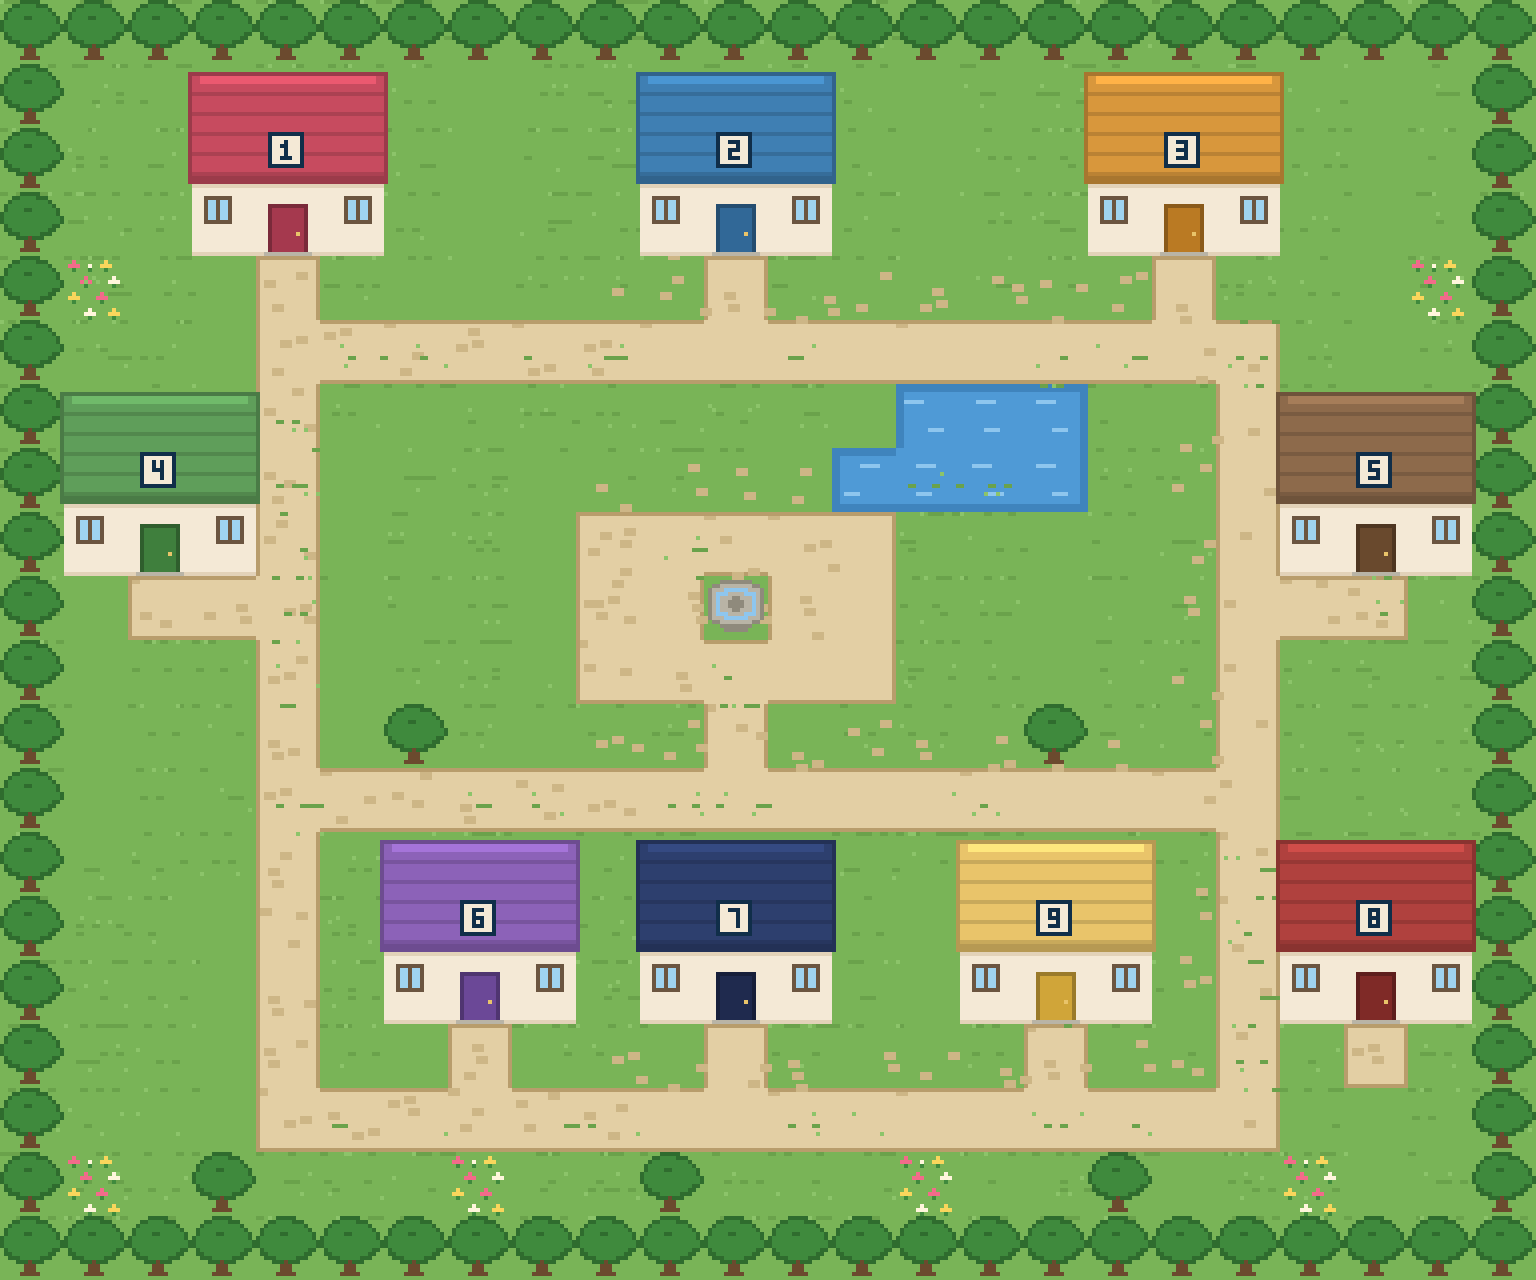
\includegraphics[width=\linewidth]{figures/art-town.png}
    \caption{The whole town, drawn in code}\label{fig:teaser-map}
  \end{subfigure}\hfill
  \begin{subfigure}[b]{0.235\textwidth}
    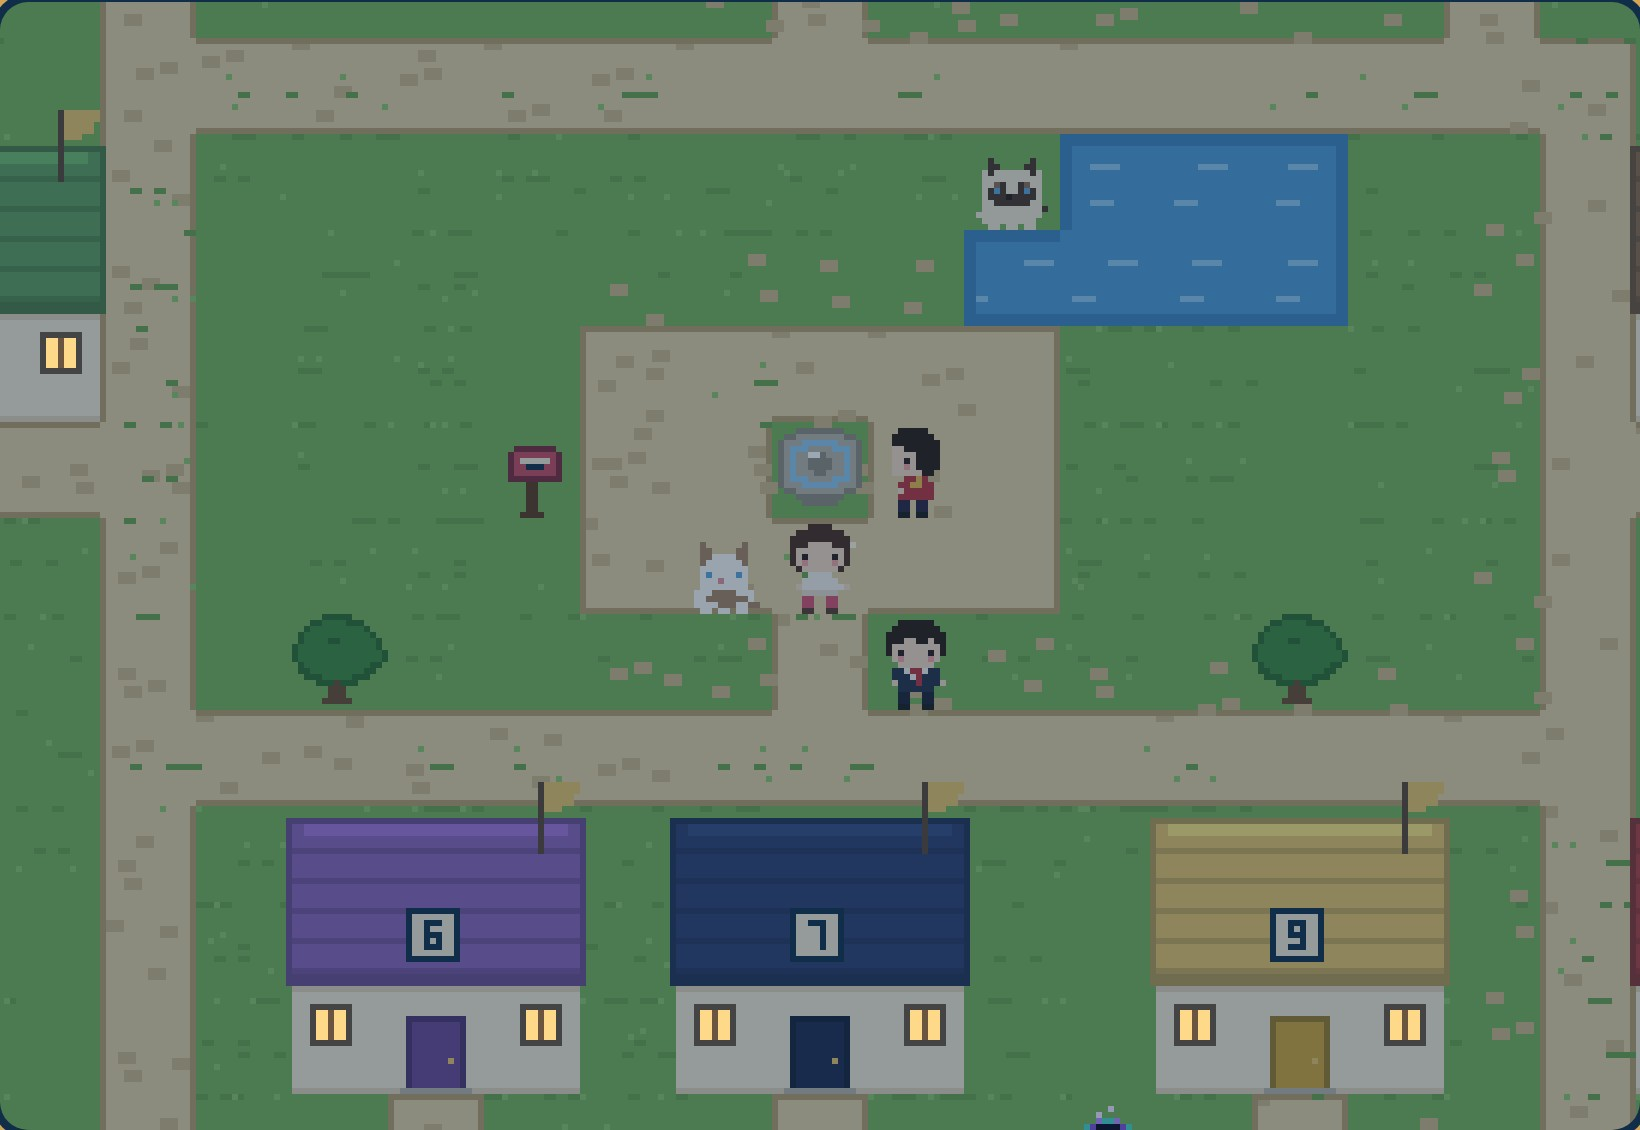
\includegraphics[width=\linewidth]{figures/town-done-canvas.jpg}\\[2pt]
    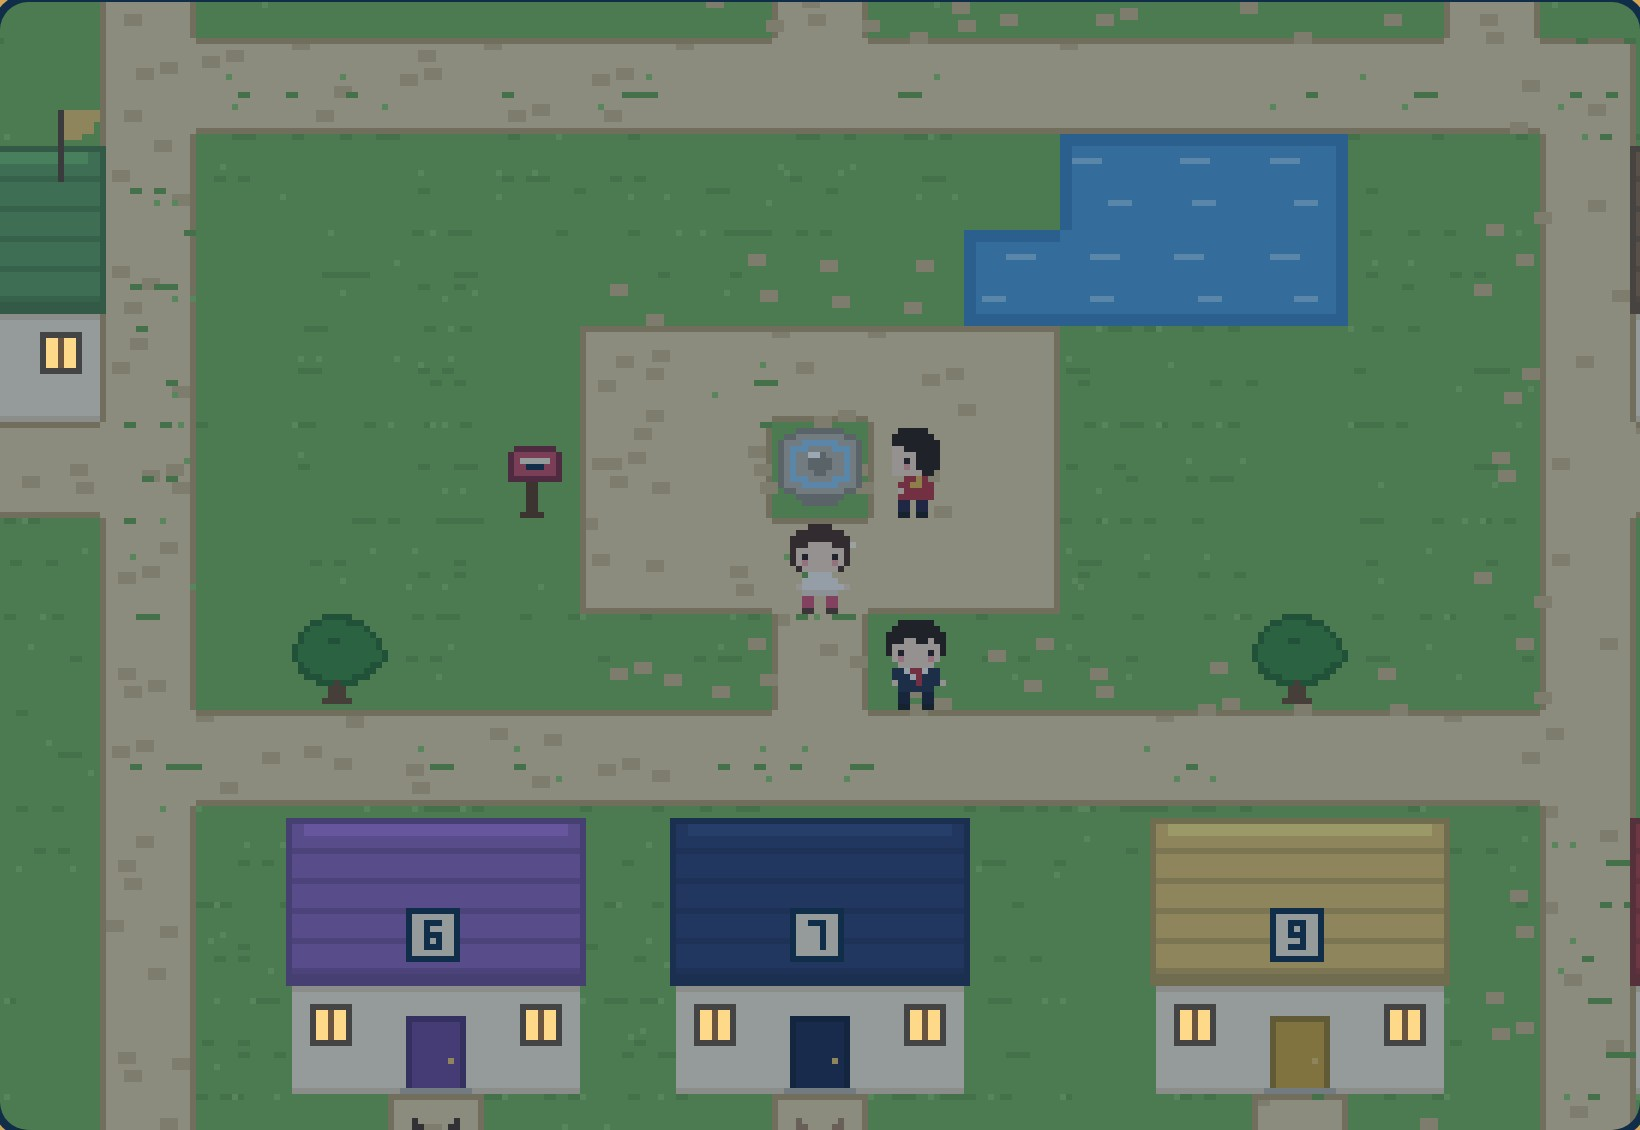
\includegraphics[width=\linewidth]{figures/town-canvas.jpg}
    \caption{The square: guide, partner, cats}\label{fig:teaser-square}
  \end{subfigure}\hfill
  \begin{subfigure}[b]{0.245\textwidth}
    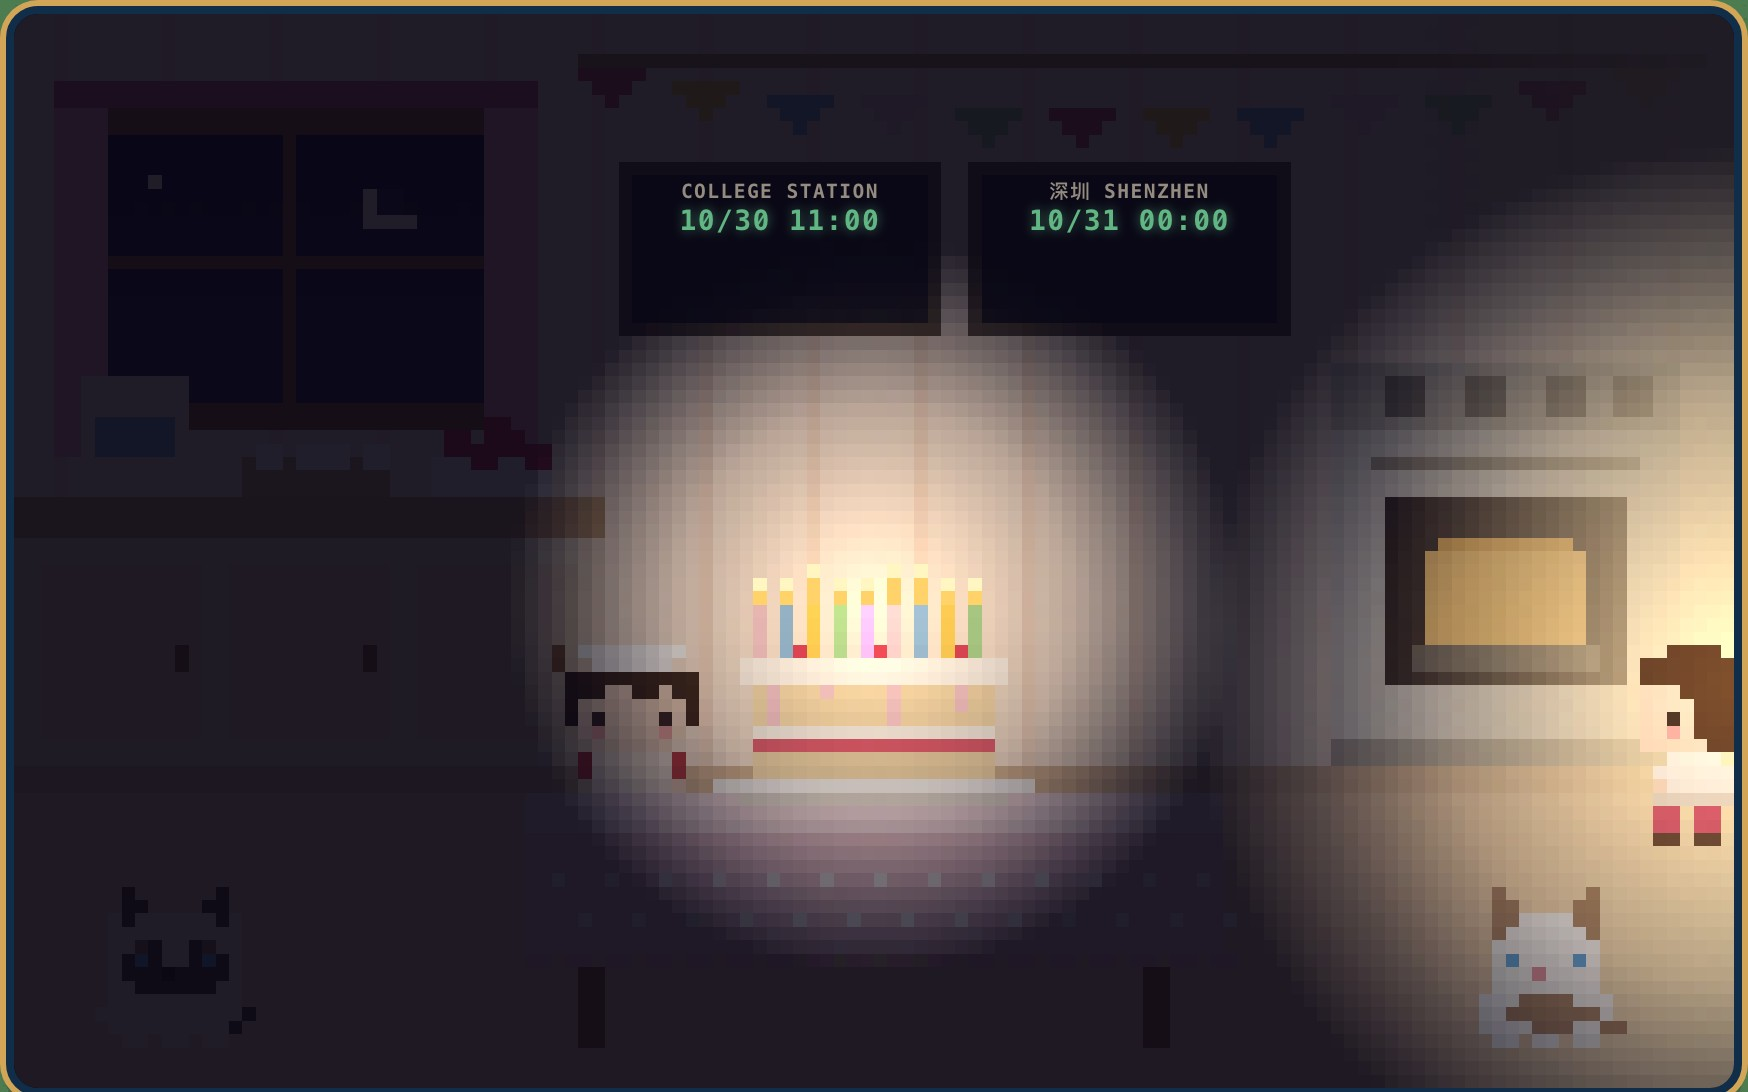
\includegraphics[width=\linewidth]{figures/bday-34.jpg}\\[2pt]
    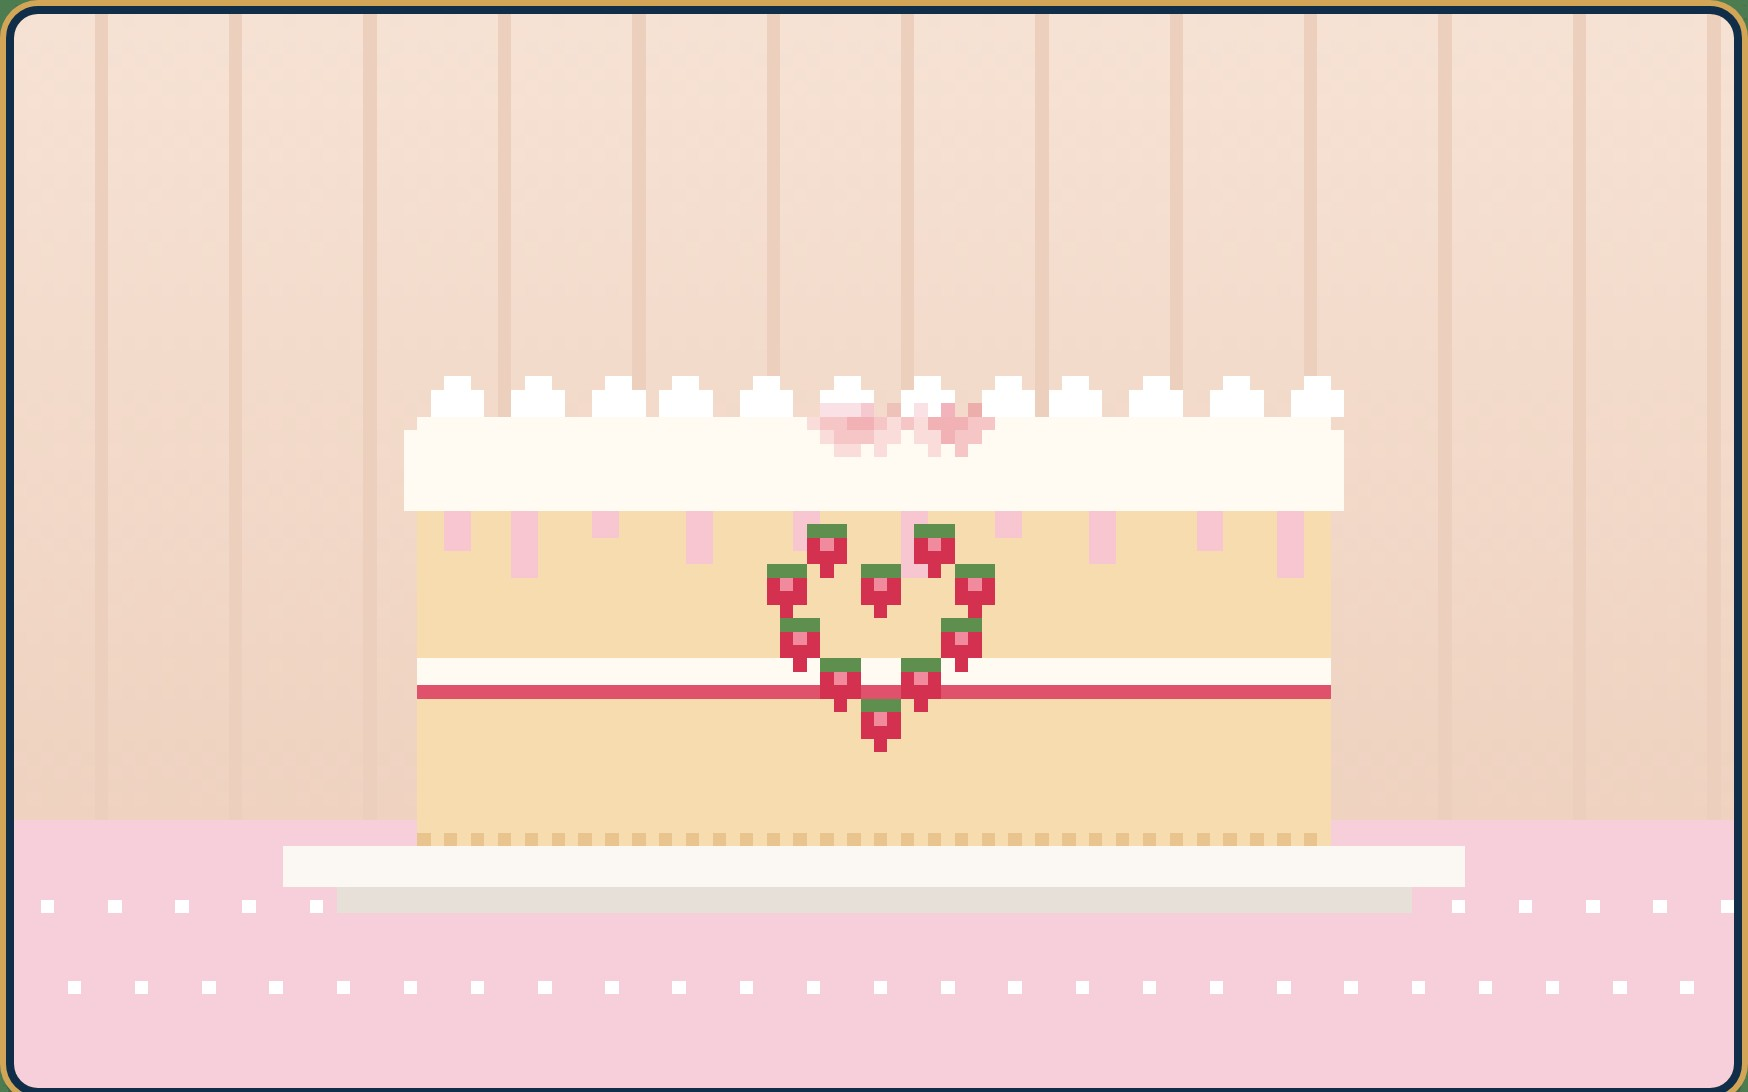
\includegraphics[width=\linewidth]{figures/bday-24.jpg}
    \caption{Prologue: the birthday cake}\label{fig:teaser-bday}
  \end{subfigure}\hfill
  \begin{subfigure}[b]{0.245\textwidth}
    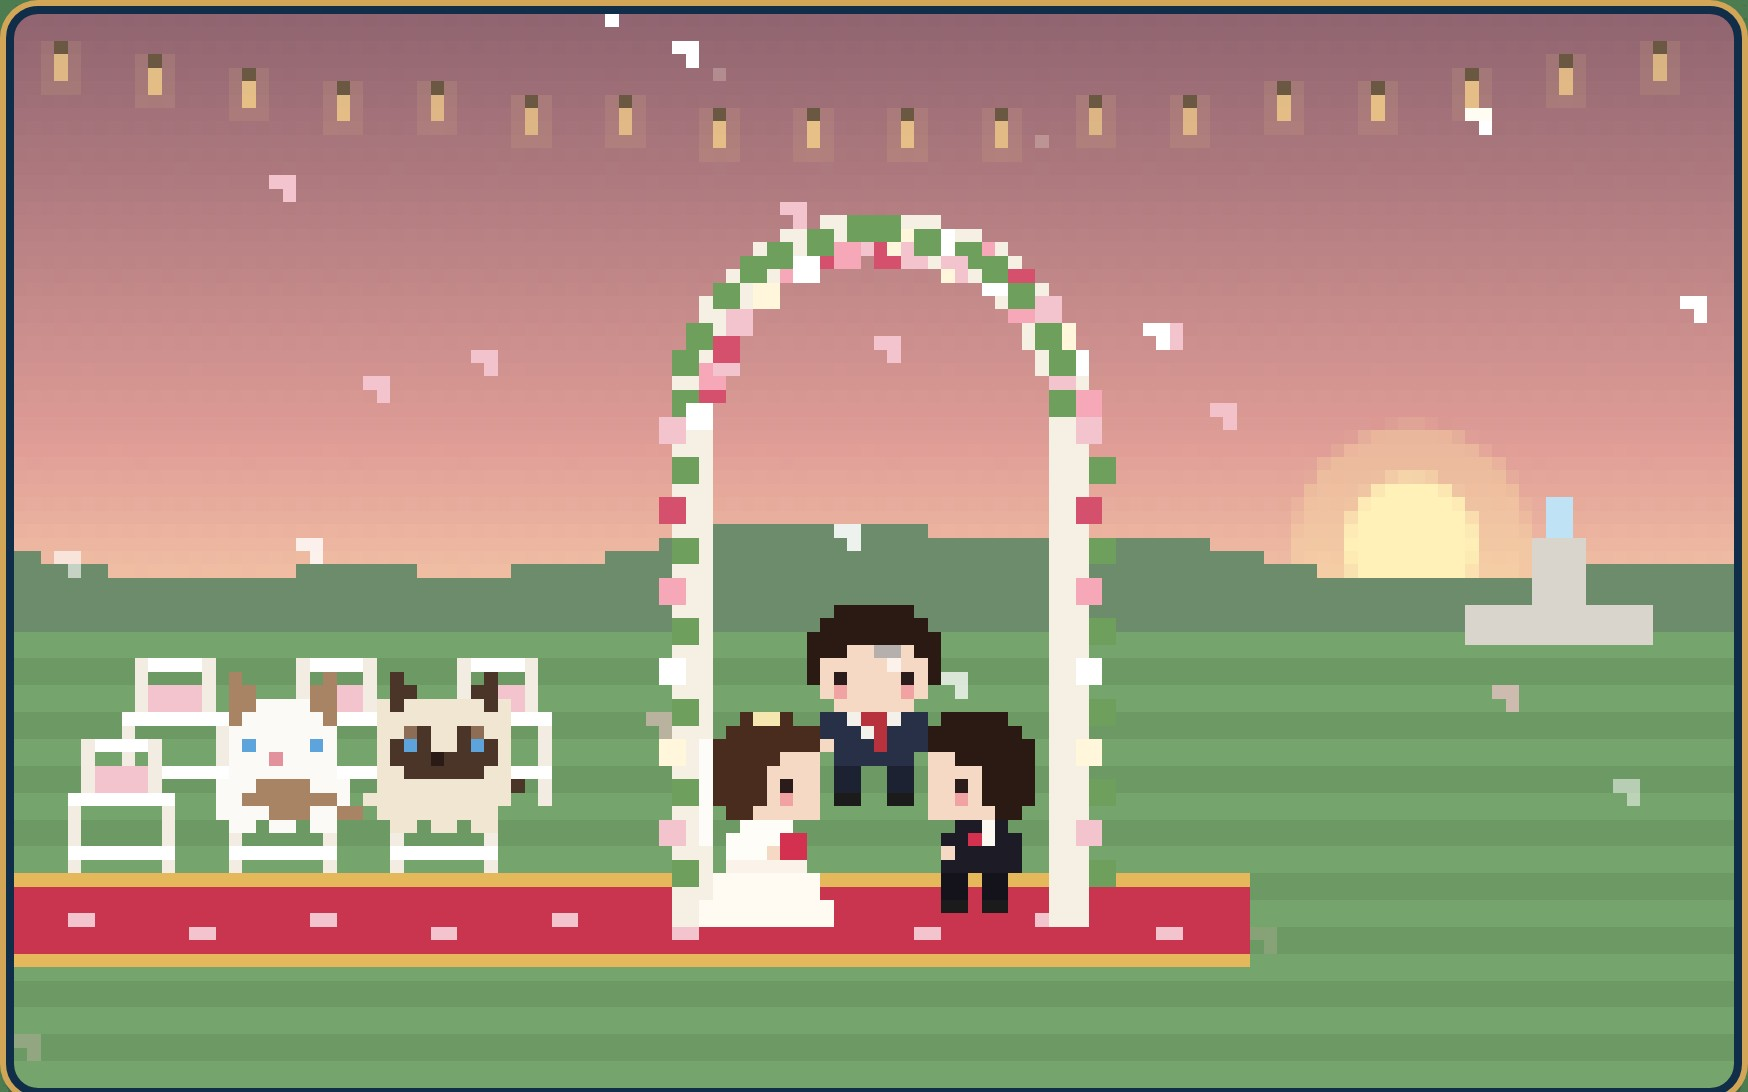
\includegraphics[width=\linewidth]{figures/wed-13.jpg}\\[2pt]
    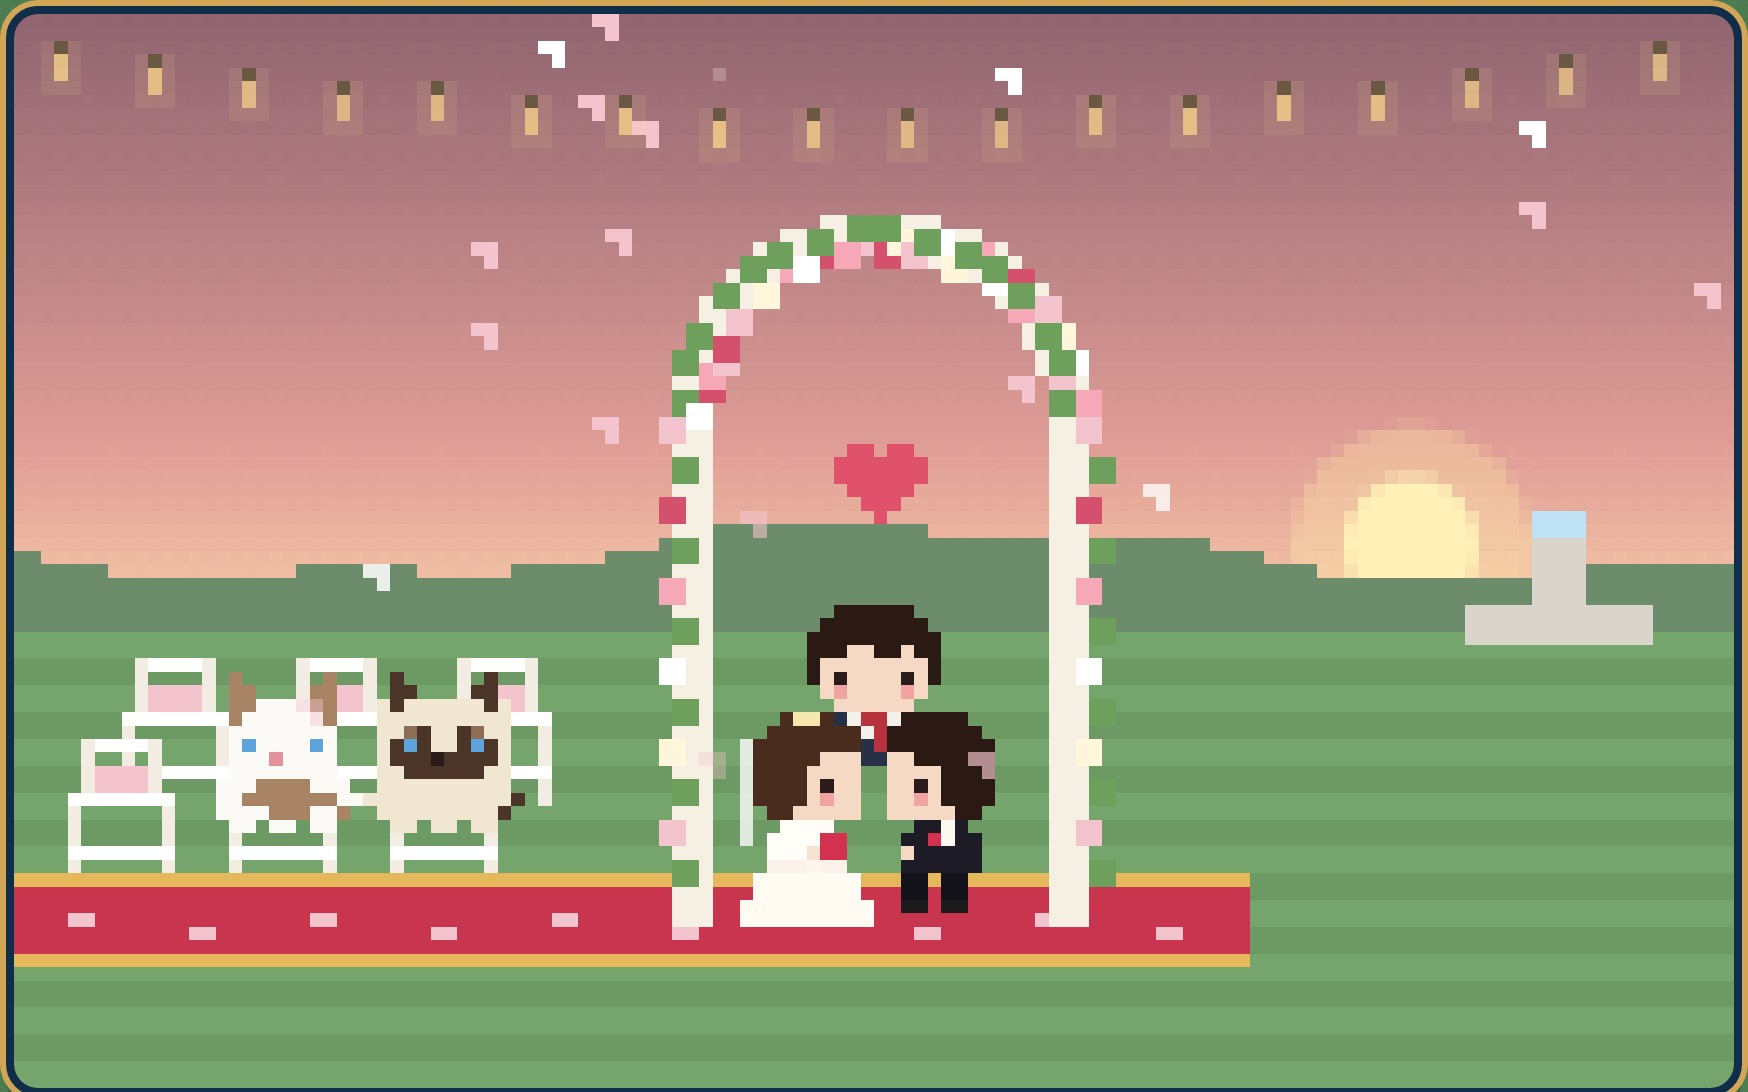
\includegraphics[width=\linewidth]{figures/wed-27.jpg}
    \caption{Finale: the wedding}\label{fig:teaser-wed}
  \end{subfigure}
  \caption{\yt{} at a glance. (a) The town map: a $24\times20$ grid of $16$-pixel tiles with nine
  numbered houses, one per level, painted entirely by code. (b) The fountain square in play, top
  after every level is cleared (gold flags, a cat sunbathing by the pond) and bottom halfway
  through; the player meets the partner, the guide Rayford and the cats. (c) The birthday
  prologue: nine candles in the dark at Shenzhen midnight, and ten strawberries set in a heart.
  (d) The wedding in the fountain garden, officiated by Rayford with the two cats as guests.}
  \Description{Four panels: a full pixel-art town map with nine coloured houses around a fountain;
  two close-ups of the square with small characters; two frames of a pixel kitchen with a lit
  birthday cake; two frames of a pixel wedding under a flower arch at sunset.}
  \label{fig:teaser}
\end{teaserfigure}

\maketitle
\hypersetup{pdftitle={MERIDIAN: Memory-Encoded Rituals for Intimacy across Distance in an Interactive, Asynchronous Neighbourhood}, pdfauthor={Jingyi Chen and Yifan Yang}}

%% ===================================================================================

\section{Introduction}
Long-distance partners use communication technologies to maintain awareness, exchange affection
and share ordinary activities~\cite{vetere2005mediating,lottridge2009sharing,neustaedter2012intimacy}.
Some report substantial intimacy despite geographical separation, but such findings do not imply
that a particular technology improves a relationship~\cite{jiang2013absence,stafford2005maintaining}.
This paper asks a narrower design question: how can a couple's shared material become an
asynchronous game, and what tensions arise when one partner authors both its narrative and its
interaction constraints?

\yt{} is a browser game developed by Yifan for Jingyi and himself. They began their relationship
on 20 September 2026 and live in Shenzhen, China, and College Station, Texas. Their clocks differed
by thirteen hours during development; the difference becomes fourteen hours when Texas observes
standard time. The game draws on shared songs, a Gomoku game, dated memories and a symbolic
hand-drawn ticket representing a planned meeting. Players navigate a pixel town whose nine houses
contain levels, while a birthday prologue, a letter and a fictional wedding organise the narrative
(Figure~\ref{fig:teaser}). The game accommodates separate visits without requiring simultaneous
participation; it does not prohibit the two people from playing at the same time.

We use \textsc{Meridian} as the name for this design case: Memory-Encoded Rituals for Intimacy
across Distance in an Interactive, Asynchronous Neighbourhood. A \emph{memory-encoded ritual}
means a scripted action whose intended significance derives from shared autobiographical material.
This is a design description, not evidence that the action becomes an established ritual in use.
Likewise, \emph{intimacy} names the intended qualities of recognition, affection and shared meaning;
we do not operationalise or measure it as an outcome. The central design move is to make a memory
shape an action or a rule, rather than only illustrate an interface.

The paper reports an artefact and a retrospective reconstruction of its development before the
recipient's planned first play on 31 October 2026. It draws on research through design and
autobiographical design, without claiming the extensive lived use associated with mature
first-person studies~\cite{zimmerman2007rtd,gaver2012expect,neustaedter2012autobiographical}.
Its contributions are:
\begin{enumerate}[leftmargin=*,itemsep=2pt,topsep=2pt]
  \item A documented design case that translates autobiographical material into nine game levels
  and staged ceremonies (Sections~\ref{sec:method} and~\ref{sec:experience}).
  \item Six situated design commitments and four traceable development episodes, with explicit
  distinctions between recorded changes, interpretations and unevaluated intentions
  (Table~\ref{tab:commitments}; Section~\ref{sec:log}).
  \item An implementation account and verification audit of local progress, manual code exchange
  and selected interface properties, together with their privacy and reliability limits
  (Section~\ref{sec:system}).
\end{enumerate}
The application of established mechanisms such as union merge is an engineering choice within
this case, not a new replication algorithm or a demonstrated intervention for relationships.

%% ===================================================================================

\section{Related Work}

\subsection{Mediating Intimacy at a Distance}
Vetere et al.\ studied how couples and families express intimacy and argued that technologies for
strong ties should support the expressive, the physical and the playful, not only the
informational~\cite{vetere2005mediating}. Hassenzahl et al.\ reviewed 143 intimacy-mediating
artefacts and grouped them into six strategies: awareness, expressivity, physicalness, gift
giving, joint action and memories~\cite{hassenzahl2012love}. Many such systems are deliberately
minimal channels, such as the Virtual Intimate Object, a single button whose meaning the couple
negotiates~\cite{kaye2006clicked}. Neustaedter and Greenberg found that some long-distance couples
leave a video call running for hours to share ``being together'' rather than to
talk~\cite{neustaedter2012intimacy}; CoupleVIBE conveyed a partner's location by
vibration~\cite{bales2011couplevibe}; SyncDecor linked everyday appliances in two
homes~\cite{tsujita2008syncdecor}. \yt{} sits in Hassenzahl's \emph{memories} and \emph{gift giving}
strategies. The comparison concerns what the interface represents: a collection of
shared references organised as tasks, rather than only a live awareness signal. This combination
should not be read as evidence that autobiographical or bespoke intimate technologies are new.

\subsection{Autobiographical and First-Person Design}
Neustaedter and Sengers defined autobiographical design as design research drawing on genuine
use by the people who built the system~\cite{neustaedter2012autobiographical}, and Desjardins
and Ball documented its tensions, including the blurred line between designer and
participant, and the intimacy of the data involved~\cite{desjardins2018tensions}. First-person
methods include situated inquiry through the researcher's own experience; a small
number of people alone does not establish methodological depth~\cite{lucero2019sample,desjardins2021firstperson}. Research through design treats the artefact itself as a carrier of
knowledge~\cite{zimmerman2007rtd,gaver2012expect}. \yt{} uses autobiographical material and developer self-testing, but the present account
precedes sustained use by the recipient. We therefore distinguish the making of the artefact
from an evaluation of living with it.

\subsection{Play, Ritual and Games for Two}
Huizinga described play as a ``magic circle'' set apart from ordinary life~\cite{huizinga1955homo};
Salen and Zimmerman made the circle a design tool~\cite{salen2004rules}; Juul argued that games
are half real rules and half fiction~\cite{juul2005halfreal}. Sicart argued that play
appropriates the world and its objects~\cite{sicart2014play}, and Isbister argued that games build
connection between players through shared action~\cite{isbister2016games}. Ludic design in HCI
values curiosity and ambiguity over task efficiency~\cite{gaver2004drift,gaver2003ambiguity}, and
slow technology designs for reflection rather than throughput~\cite{hallnas2001slow,odom2012technology}.
Aron et al.'s procedure for generating closeness through escalating mutual
disclosure~\cite{aron1997closeness} is, in a sense, a level structure. \yt{} takes the game form
literally: locks, levels, a guide, a prologue and a finale. Bespoke ritual technologies
already explore connection across distance~\cite{kirk2016ritual}. Our case instead organises
selected memories and imagined futures as a sequence of game actions. Whether that sequence
becomes meaningful ritual requires evidence from use.


\subsection{Local-First and Backend-Free Progress}
Local-first software seeks to combine collaboration with user control and durable access to
data~\cite{kleppmann2019localfirst}. State-based conflict-free replicated data types (CRDTs)
converge when replicas combine compatible state through an appropriate merge; the grow-only set
uses union~\cite{shapiro2011crdt}. \yt{} adopts this operation for level completion and exchanges
state manually. It supports local progress, rather than implementing every local-first ideal.
Static hosting, remote media and browser-dependent recognition remain part of its infrastructure.
Keeping progress local also does not protect personal images that are distributed as static
assets; visual content can expose location information~\cite{yang2024geolocator}.

%% ===================================================================================

\section{Design Context and Method}\label{sec:method}

\subsection{The Two of Us}
Table~\ref{tab:dates} lists the dates that the system encodes. The couple speak Mandarin to each
other; Yifan works in English, Jingyi in Chinese and English. Both use phones as their main
devices, and Jingyi's network in mainland China blocks some services (YouTube, Google Fonts) that
Yifan's does not. These circumstances motivated bilingual text, alternative media providers and a
phone-oriented interface. They are design requirements, not verified guarantees of regional
availability or cross-device compatibility.

\begin{table}[t]
  \caption{Key dates encoded in the system (\code{src/core/config.ts}).}
  \label{tab:dates}
  \small
  \begin{tabular}{@{}lp{0.62\columnwidth}@{}}
    \toprule
    Date & Moment \\
    \midrule
    2026-09-20 & We met; day 1 of every counter in the town \\
    2026-09-25 & Yifan's birthday (Libra) \\
    2026-10-17 & First video call; the hand-drawn ticket CYF925 \\
    2026-10-23 & First Gomoku game, on a Zoom whiteboard \\
    2026-10-24 & First commit of \yt{} \\
    2026-10-31 & Jingyi's birthday (Scorpio); intended first recipient play \\
    2027-02-05 & Planned meeting; symbolic ticket CYF925; countdown target \\
    \bottomrule
  \end{tabular}
\end{table}


\subsection{Scope, Corpus and Reconstruction}
The design corpus comprises 109 commits dated 24--28 October 2026, 28 changelog entries from
version 0.1.0 to 1.17.0, and three specifications for the site, quest and town. The development
cut-off is commit \code{55440ae}; the manuscript inspected for revision is commit \code{94ce914}.
Yifan directed the design, supplied the autobiographical material and tested both player roles,
with substantial implementation assistance from an AI coding assistant. Jingyi is the intended
recipient. This account reports no interview, diary, recipient play session or relationship measure.
The two intended players therefore do not constitute a two-participant evaluation sample.

For the present reconstruction, we inspect the documented changes underlying four episodes:
replacing Pictionary, changing the ring's completion condition, correcting represented routines,
and revising the entry gate (Section~\ref{sec:log}). Each episode links a source change to an
interpretation of the design trade-off. The selection illustrates decisions discussed in this
paper; it is not an exhaustive coding of all commits or an independently coded thematic analysis.
Version history establishes what changed and when, but cannot establish the recipient's response
or the designer's unrecorded motivation. Interpretations remain open to alternative readings.

\subsection{Knowledge Claims and Positionality}
Research through design can make an artefact and its rationale available for scrutiny without
claiming a universal solution~\cite{zimmerman2007rtd,gaver2012expect}. First-person inquiry also
requires attention to whose experience becomes evidence~\cite{desjardins2018tensions,desjardins2021firstperson}.
Here, the designer's familiarity with the relationship informs the content but cannot substitute
for the other partner's perspective. Technical checks establish selected implementation properties.
The six commitments below are situated design choices reconstructed from the artefact and log;
they are neither empirically validated principles nor measured determinants of intimacy.

\subsection{Six Design Commitments}
We articulate six commitments from this reconstruction of the five-day development period. Table~\ref{tab:commitments} maps each to
the mechanisms that realise it.


\begin{description}[leftmargin=0pt,labelwidth=0pt,labelsep=0pt,style=nextline,itemsep=2pt,topsep=2pt,font=\normalfont\scshape]
  \item[D1 Memory-derived mechanics.] Selected memories and shared references shape tasks.
  The Gomoku level reworks a prior game; the ring represents an imagined future rather than a past event.
  \item[D2 Staged access.] Ordered levels and door entry organise the narrative. These controls
  shape normal play, but are not security barriers or evidence of meaningful effort.
  \item[D3 Local progress.] Completion state is stored on-device and shared through a code,
  without an author-operated progress backend. External services remain involved in other features.
  \item[D4 Bilingual coverage.] Both dictionaries contain non-empty values for the same keys.
  Structural tests do not establish semantic equivalence or accessibility in either language.
  \item[D5 Code-defined pixel art.] Town tiles and character sprites are generated in code.
  Photographs, audio, rendered rings and other assets have separate provenance and reuse conditions.
  \item[D6 Delayed narrative disclosure.] A lexical test checks selected dictionary entries for
  explicit references to the finale. It does not prove that every interface or asset preserves surprise.

\end{description}

\begin{table}[t]
  \caption{Design commitments and the mechanisms that realise them.}
  \label{tab:commitments}
  \small
  \begin{tabular}{@{}p{0.30\columnwidth}p{0.62\columnwidth}@{}}
    \toprule
    Commitment & Realised by \\
    \midrule
    \dc{1} Memory-derived mechanics & Memories, cultural references and imagined futures become tasks (Table~\ref{tab:levels}) \\
    \dc{2} Earned access & Ordered level registry; router guard; door-only entry; cats guarding the next locks \\
    \dc{3} Local progress & \code{localStorage} per player; grow-only set; progress codes; PWA offline cache \\
    \dc{4} Bilingual coverage & Matching non-empty dictionary keys; no independent language-quality evaluation \\
    \dc{5} Drawn in code & Sprites and tiles as strings; banner and icons generated from them \\
    \dc{6} Delayed disclosure & Lexical test over eligible dictionary keys, with explicit exclusions \\
    \bottomrule
  \end{tabular}
\end{table}

%% ===================================================================================
\section{The Experience}\label{sec:experience}

\subsection{The Front Door}
The site opens on a single question. The answer, a date both players know, is accepted in
several spellings: its digits are compared against SHA-256 hashes~\cite{fips1804}. Hashing
changes the comparison representation, but the date also appears in the application's narrative
and source material; it is not a secret protected by cryptography. Behind it is a dashboard that lists everything the couple
build under the domain (Figure~\ref{fig:front}a), of which \yt{} is the first. Choosing the town
asks \emph{Who are you?} (Figure~\ref{fig:front}b). Progress is kept per player on each device,
so both can play on one phone.

\begin{figure}[t]
  \centering
  \begin{subfigure}[b]{0.49\columnwidth}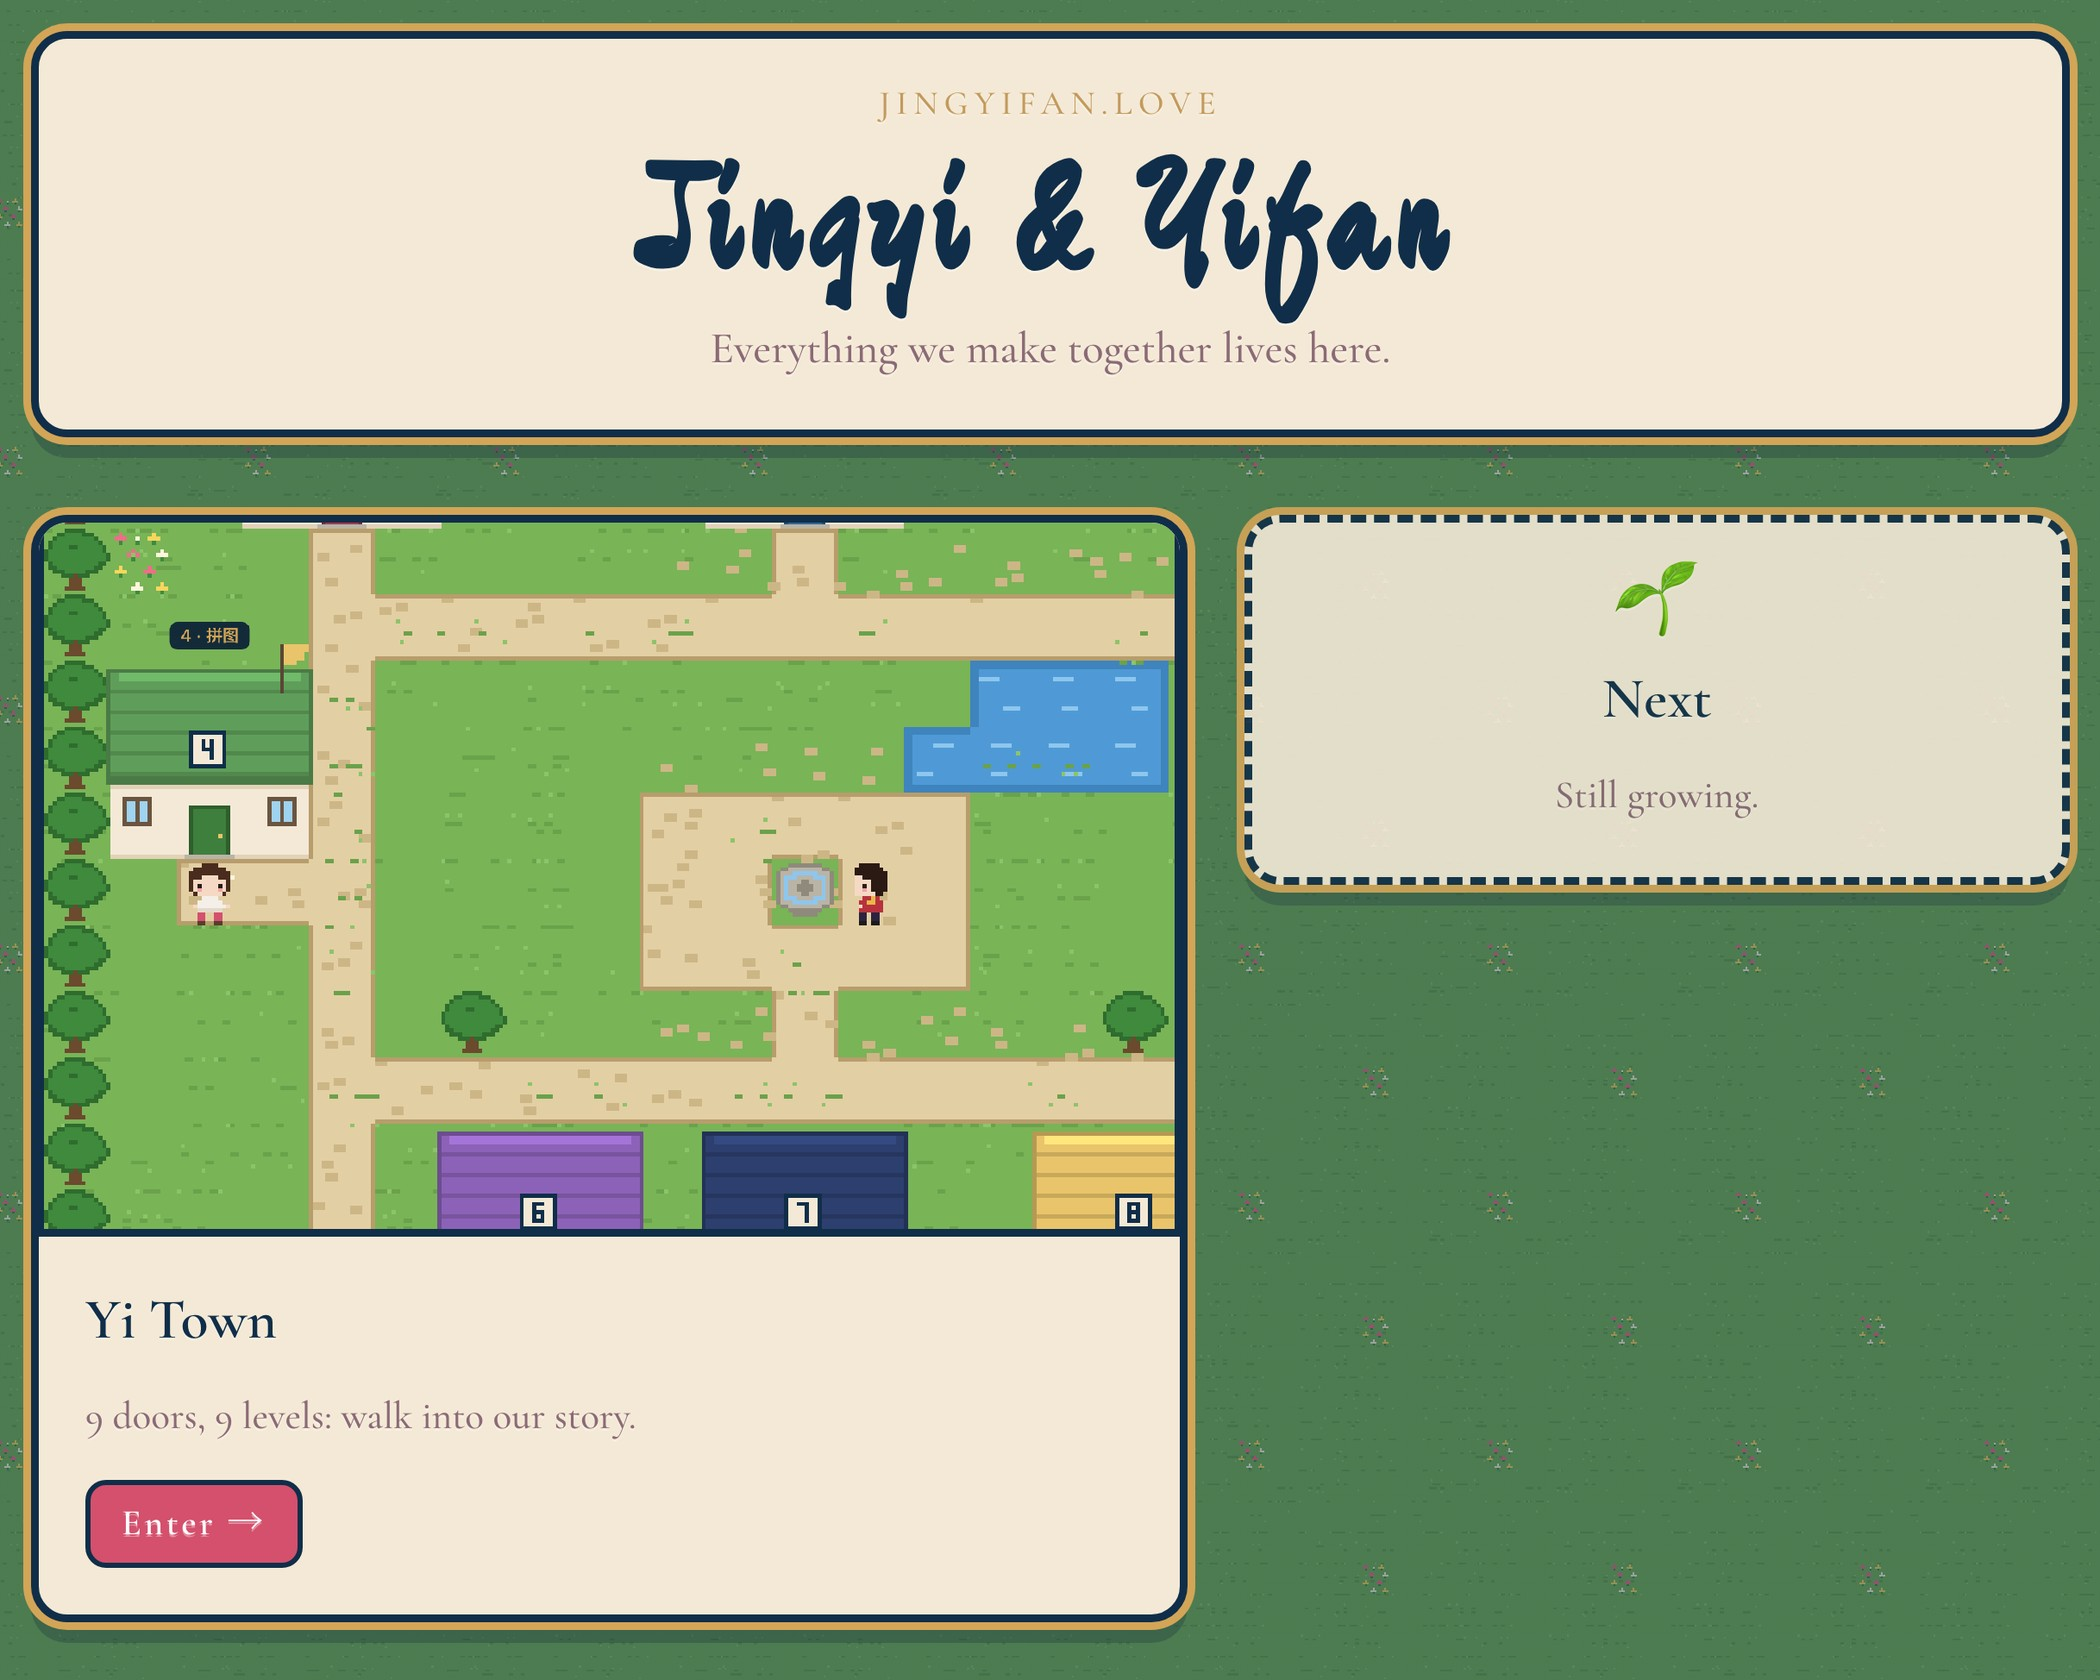
\includegraphics[width=\linewidth]{figures/page-dashboard.jpg}\caption{Dashboard}\end{subfigure}\hfill
  \begin{subfigure}[b]{0.49\columnwidth}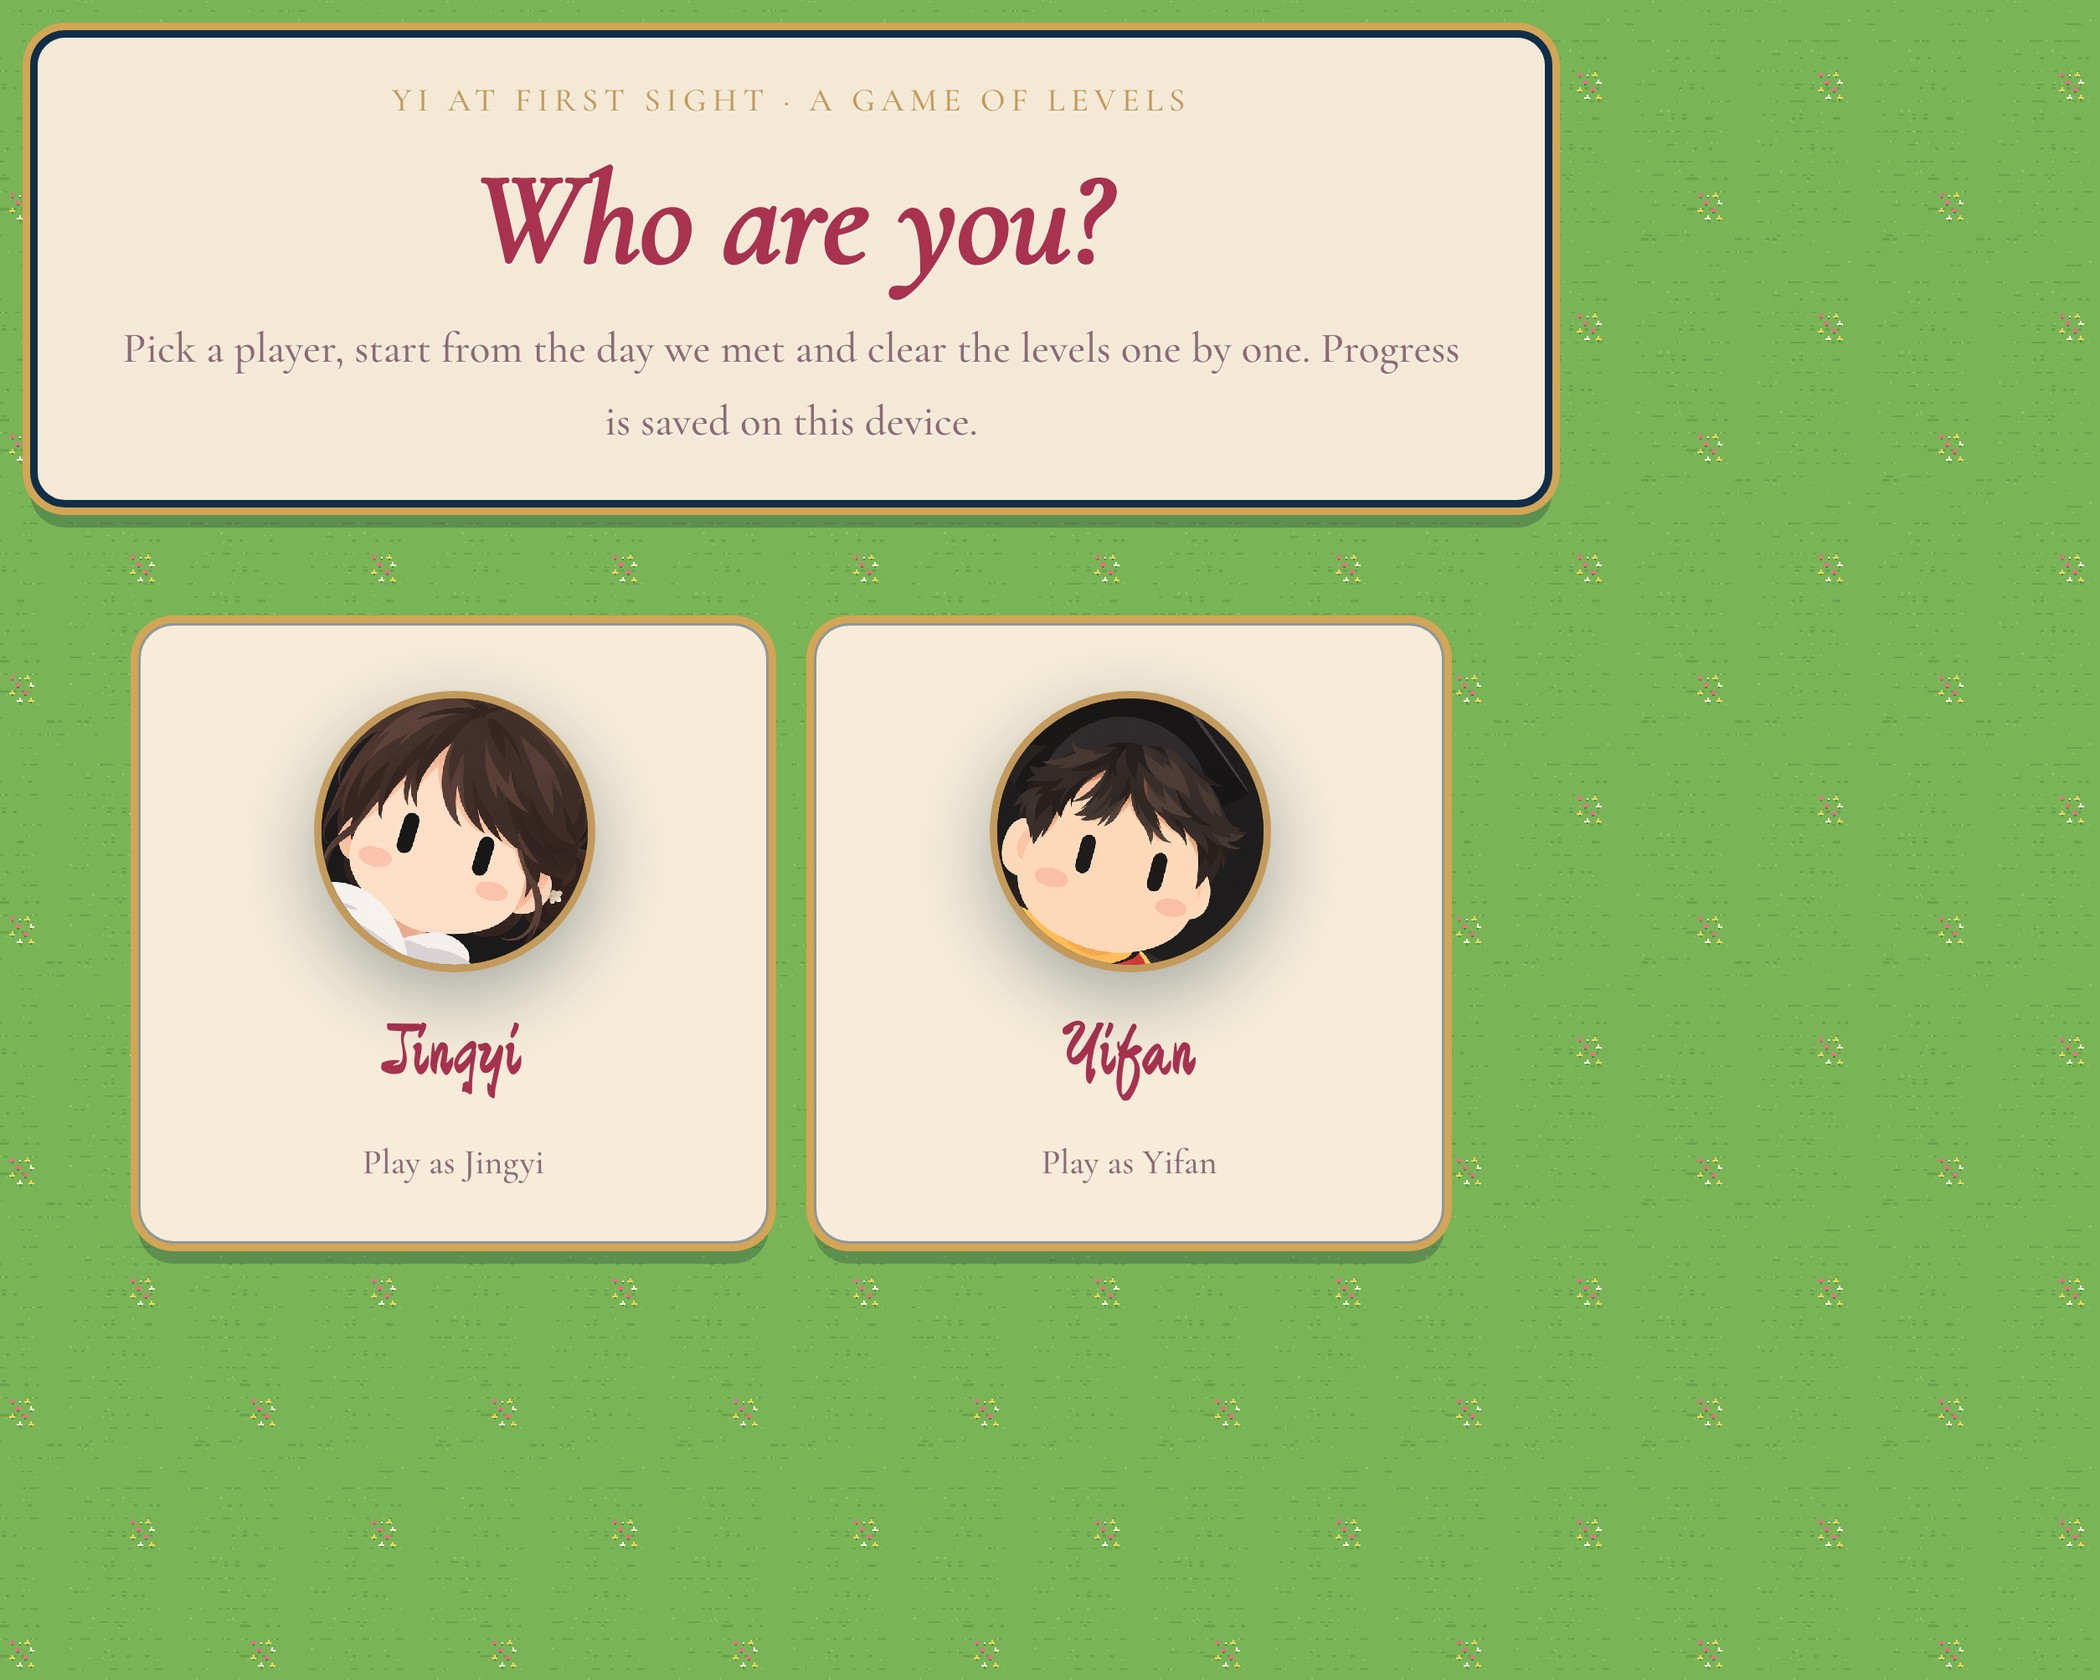
\includegraphics[width=\linewidth]{figures/page-start.jpg}\caption{Pick a player}\end{subfigure}\\[3pt]
  \begin{subfigure}[b]{0.49\columnwidth}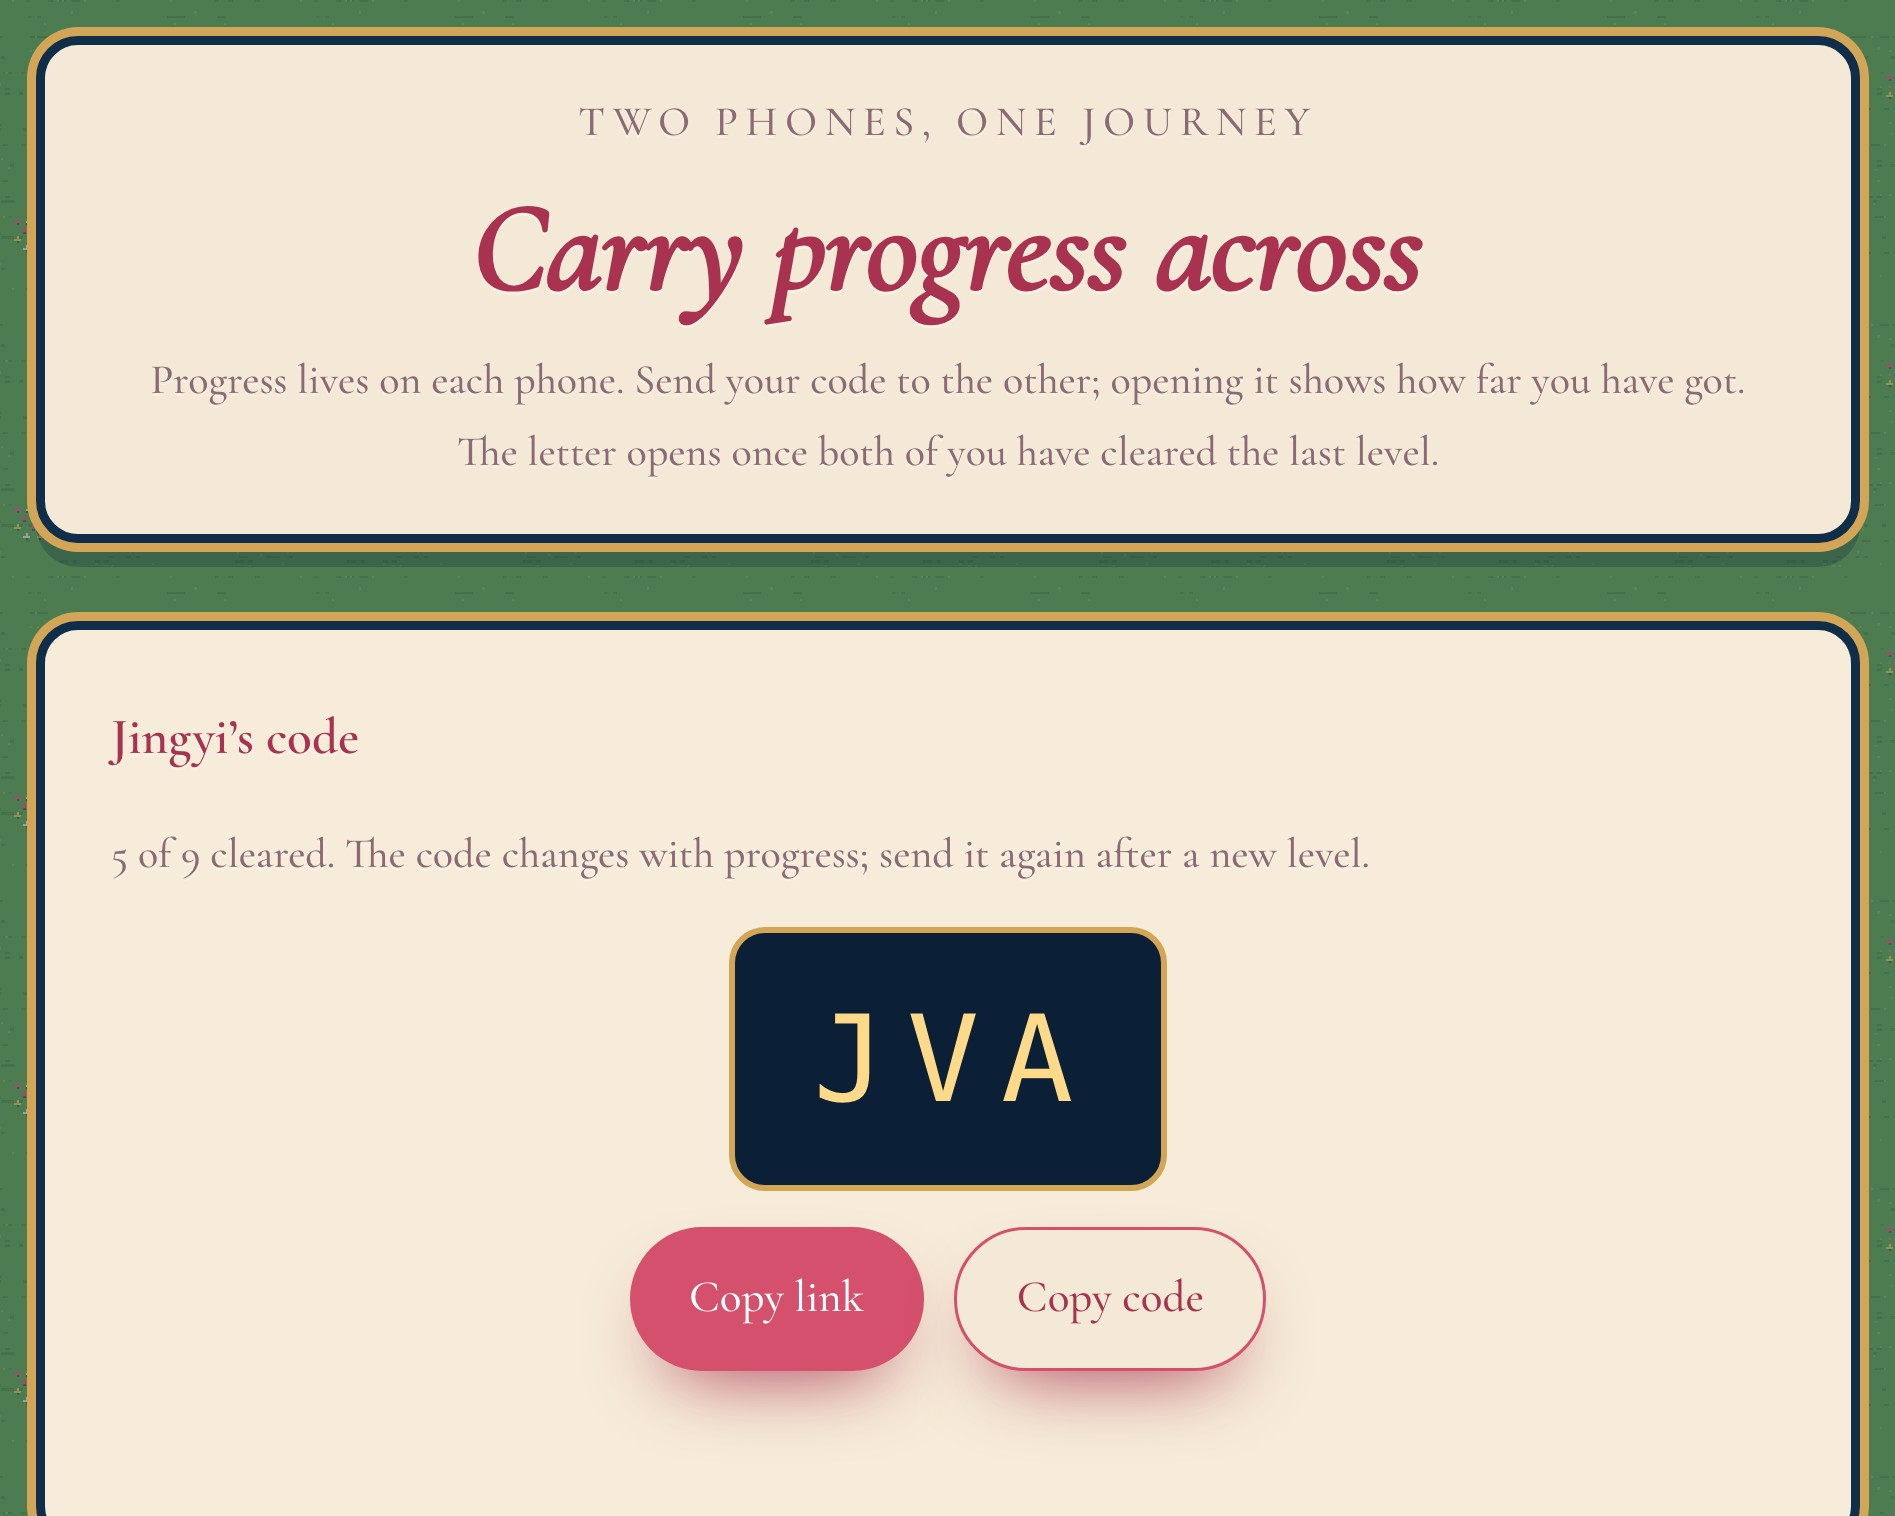
\includegraphics[width=\linewidth]{figures/page-sync.jpg}\caption{Progress code}\end{subfigure}\hfill
  \begin{subfigure}[b]{0.49\columnwidth}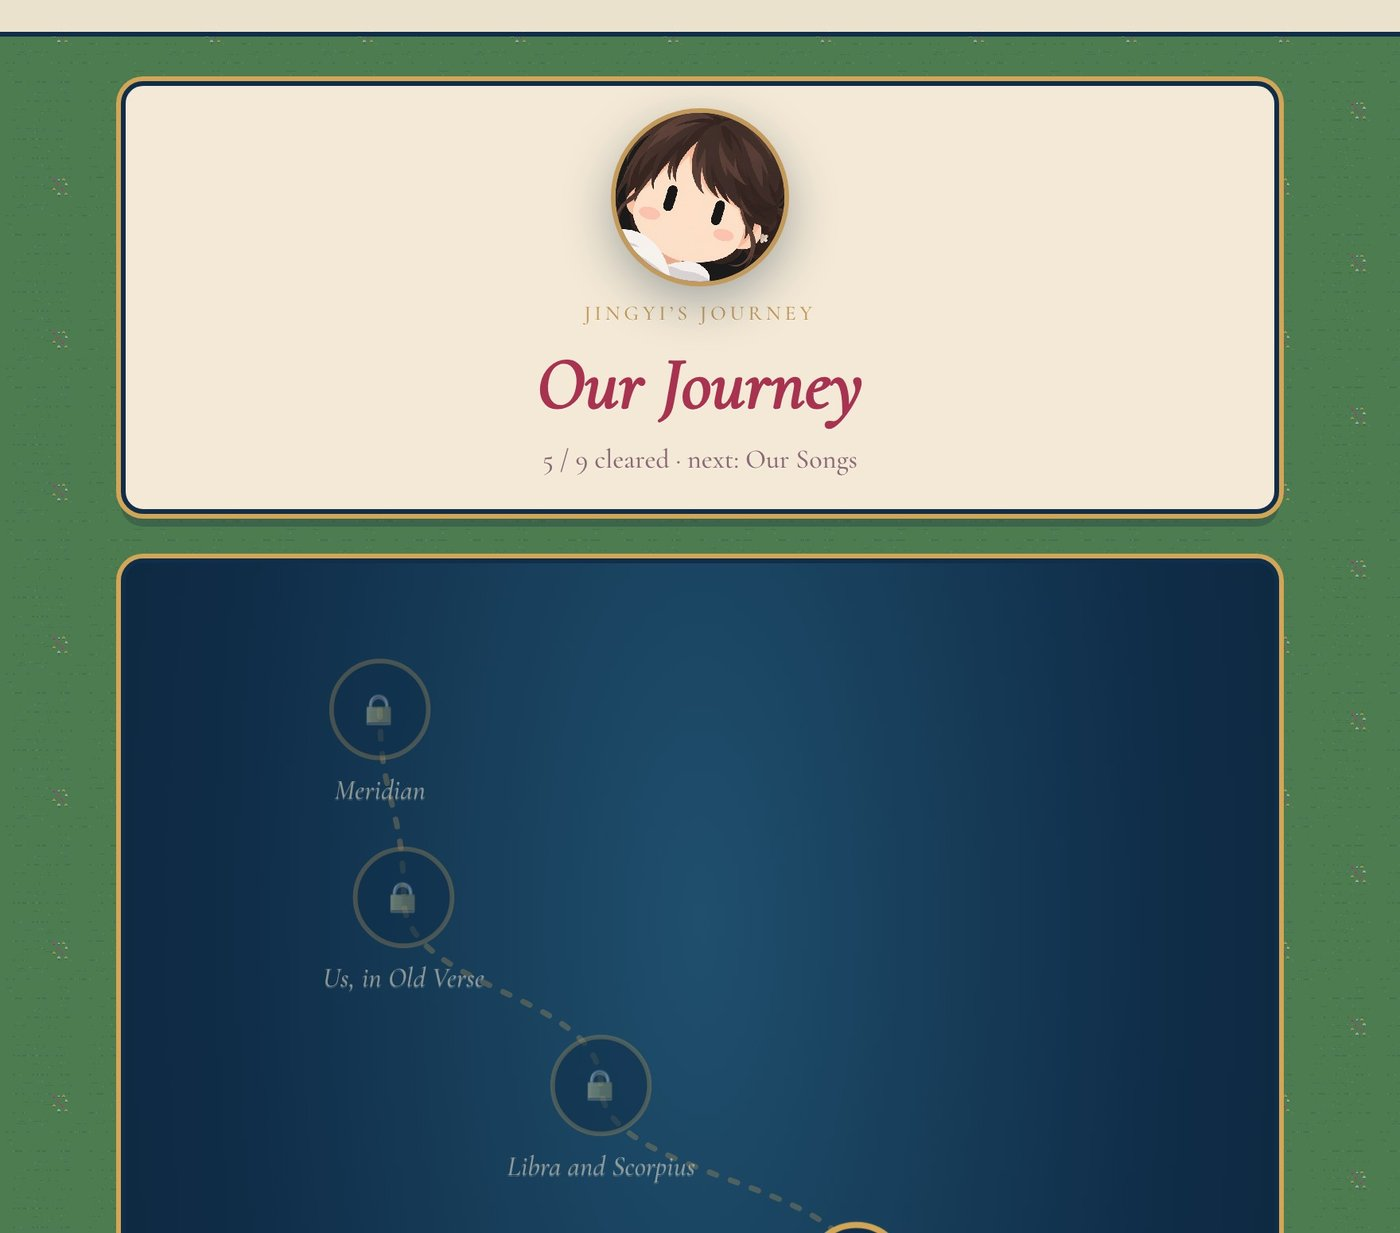
\includegraphics[width=\linewidth]{figures/page-journey.jpg}\caption{The journey list}\end{subfigure}
  \caption{Around the town. (a) The dashboard lists every product under the domain. (b) Each device
  keeps one progress per player. (c) Progress crosses phones as a code (here \code{JVA}). (d) The
  journey as a list, for players who prefer it to the map.}
  \Description{Four screenshots in cream and navy on a green pixel meadow: a dashboard card with a
  map thumbnail; two avatar cards; a large three-letter code; a handwritten-style letter.}
  \label{fig:front}
\end{figure}

\subsection{The Town}
The town (Figure~\ref{fig:teaser-map}) is a $24\times20$ grid of $16\times16$-pixel tiles. Paths
connect nine houses around a fountain square and a pond. Each roof has its own colour and its
level number, and a cleared house flies a gold flag. The player moves with the arrow keys, by
tapping a tile (the avatar walks a shortest path to it), or with an on-screen d-pad. Walking into
a door opens a talk box with the level's one-line story, for example ``Our first game was on a Zoom
whiteboard. Now you place the last stone.''

Four kinds of character live in the town (Figure~\ref{fig:sprites}). The \emph{partner} waits by
the fountain and reports how far they have got (``I am waiting here. I have cleared 5 levels.
You?''). \emph{Rayford}, Yifan in a suit, is a scripted guide south of the fountain: he explains
the project, lists the levels, hints at the next one and walks the player to its door. Two Ragdoll
cats, \emph{Coffee} (\zh{咖啡}) and \emph{Duoduo} (\zh{哆哆}), guard the locks: Coffee sits at the next
locked door and Duoduo at the one after. When a door opens they walk to their new posts, and with
nothing left to guard they sunbathe by the pond. Bumping into a cat shows a photo of the real cat.
Two signposts lead out of the square to the two cities (Section~\ref{sec:days}), and a red mailbox
holds voice notes the partner has left.

The sky follows the clock in the player's own city: Jingyi walks the town in Shenzhen time and
Yifan in College Station time, so at the same instant one sees noon and the other sees lit windows
under a night wash. The whole site stands on the same pixel meadow, and every heading is a cream
sign in the town's palette, so leaving a house never leaves the world.

\begin{figure}[t]
  \centering
  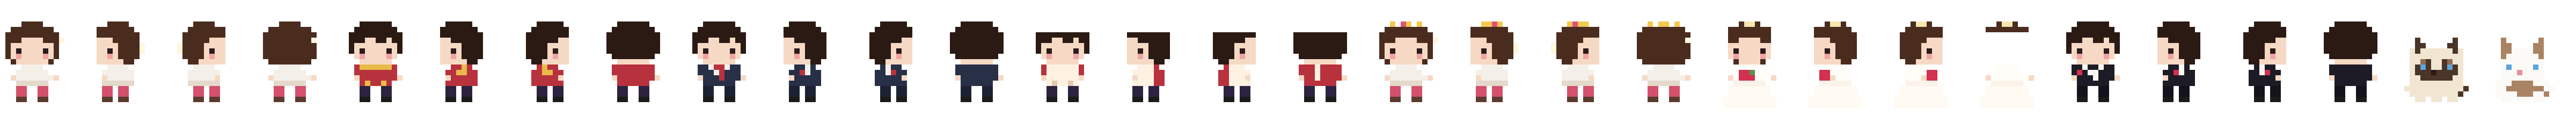
\includegraphics[width=\columnwidth]{figures/art-sprites.png}
  \caption{Every character in \yt{} is a string of characters in the source. From left: Jingyi,
  Yifan, Rayford, Yifan as the baker, Jingyi crowned, the bride and the groom (four facings each),
  then the cats Coffee and Duoduo. Bodies are $12\times12$ pixels over four rows of shared legs.}
  \Description{A row of tiny pixel-art characters seen from four sides, followed by two pixel cats.}
  \label{fig:sprites}
\end{figure}

\subsection{Nine Levels}
Table~\ref{tab:levels} lists the levels with their source memory, mechanic and input modality,
and Figure~\ref{fig:levels} shows them in play.

\begin{table*}[t]
  \caption{The nine levels: autobiographical material, shared references and imagined futures become tasks (\dc{1}). Modalities: \emph{V}~voice,
  \emph{T}~touch or pointer, \emph{C}~camera, \emph{K}~keyboard alternative available.}
  \label{tab:levels}
  \small
  \begin{tabular}{@{}clp{0.25\textwidth}p{0.36\textwidth}cl@{}}
    \toprule
    \# & Level & Design material & Task (clear condition) & Input & Data \\
    \midrule
    1 & The Day We Met & 20 September 2026; the vow & Answer a question, then say \emph{\zh{我爱你，<name>，我愿意}} aloud; homophones of the name accepted & V/K & 1 vow per player \\
    2 & Love Map & Where each studied; where they will meet & Name six street views; each right answer drops a heart on the map to collect & T & 6 places \\
    3 & Tattoo & A promise to write on each other & Handwrite a line on an arm or shoulder, then ``ink it'' & T & strokes \\
    4 & Moments & The first 40 days & Order five memories, then reassemble a $3\times3$ portrait of the partner & T & 8 memories \\
    5 & Gomoku & First game on a Zoom whiteboard & Ten win-in-one endgames; the ten answers form a heart & T & 10 positions \\
    6 & Our Songs & The six songs they share & Hear a passage, pick the title from four & T & 6 songs \\
    7 & Libra and Scorpius & Their birth signs, neighbours in the sky & Join 21 stars along 20 edges & T/K & J2000 positions \\
    8 & Us, in Old Verse & Classical love poetry & Restore the missing half-line of five poems character by character & T & 5 poems \\
    9 & Meridian & What comes next & Try the ring on through the camera and take a photo & C & 3 GLB models \\
    \bottomrule
  \end{tabular}
\end{table*}

\begin{figure*}[t]
  \centering
  \begin{subfigure}[b]{0.24\textwidth}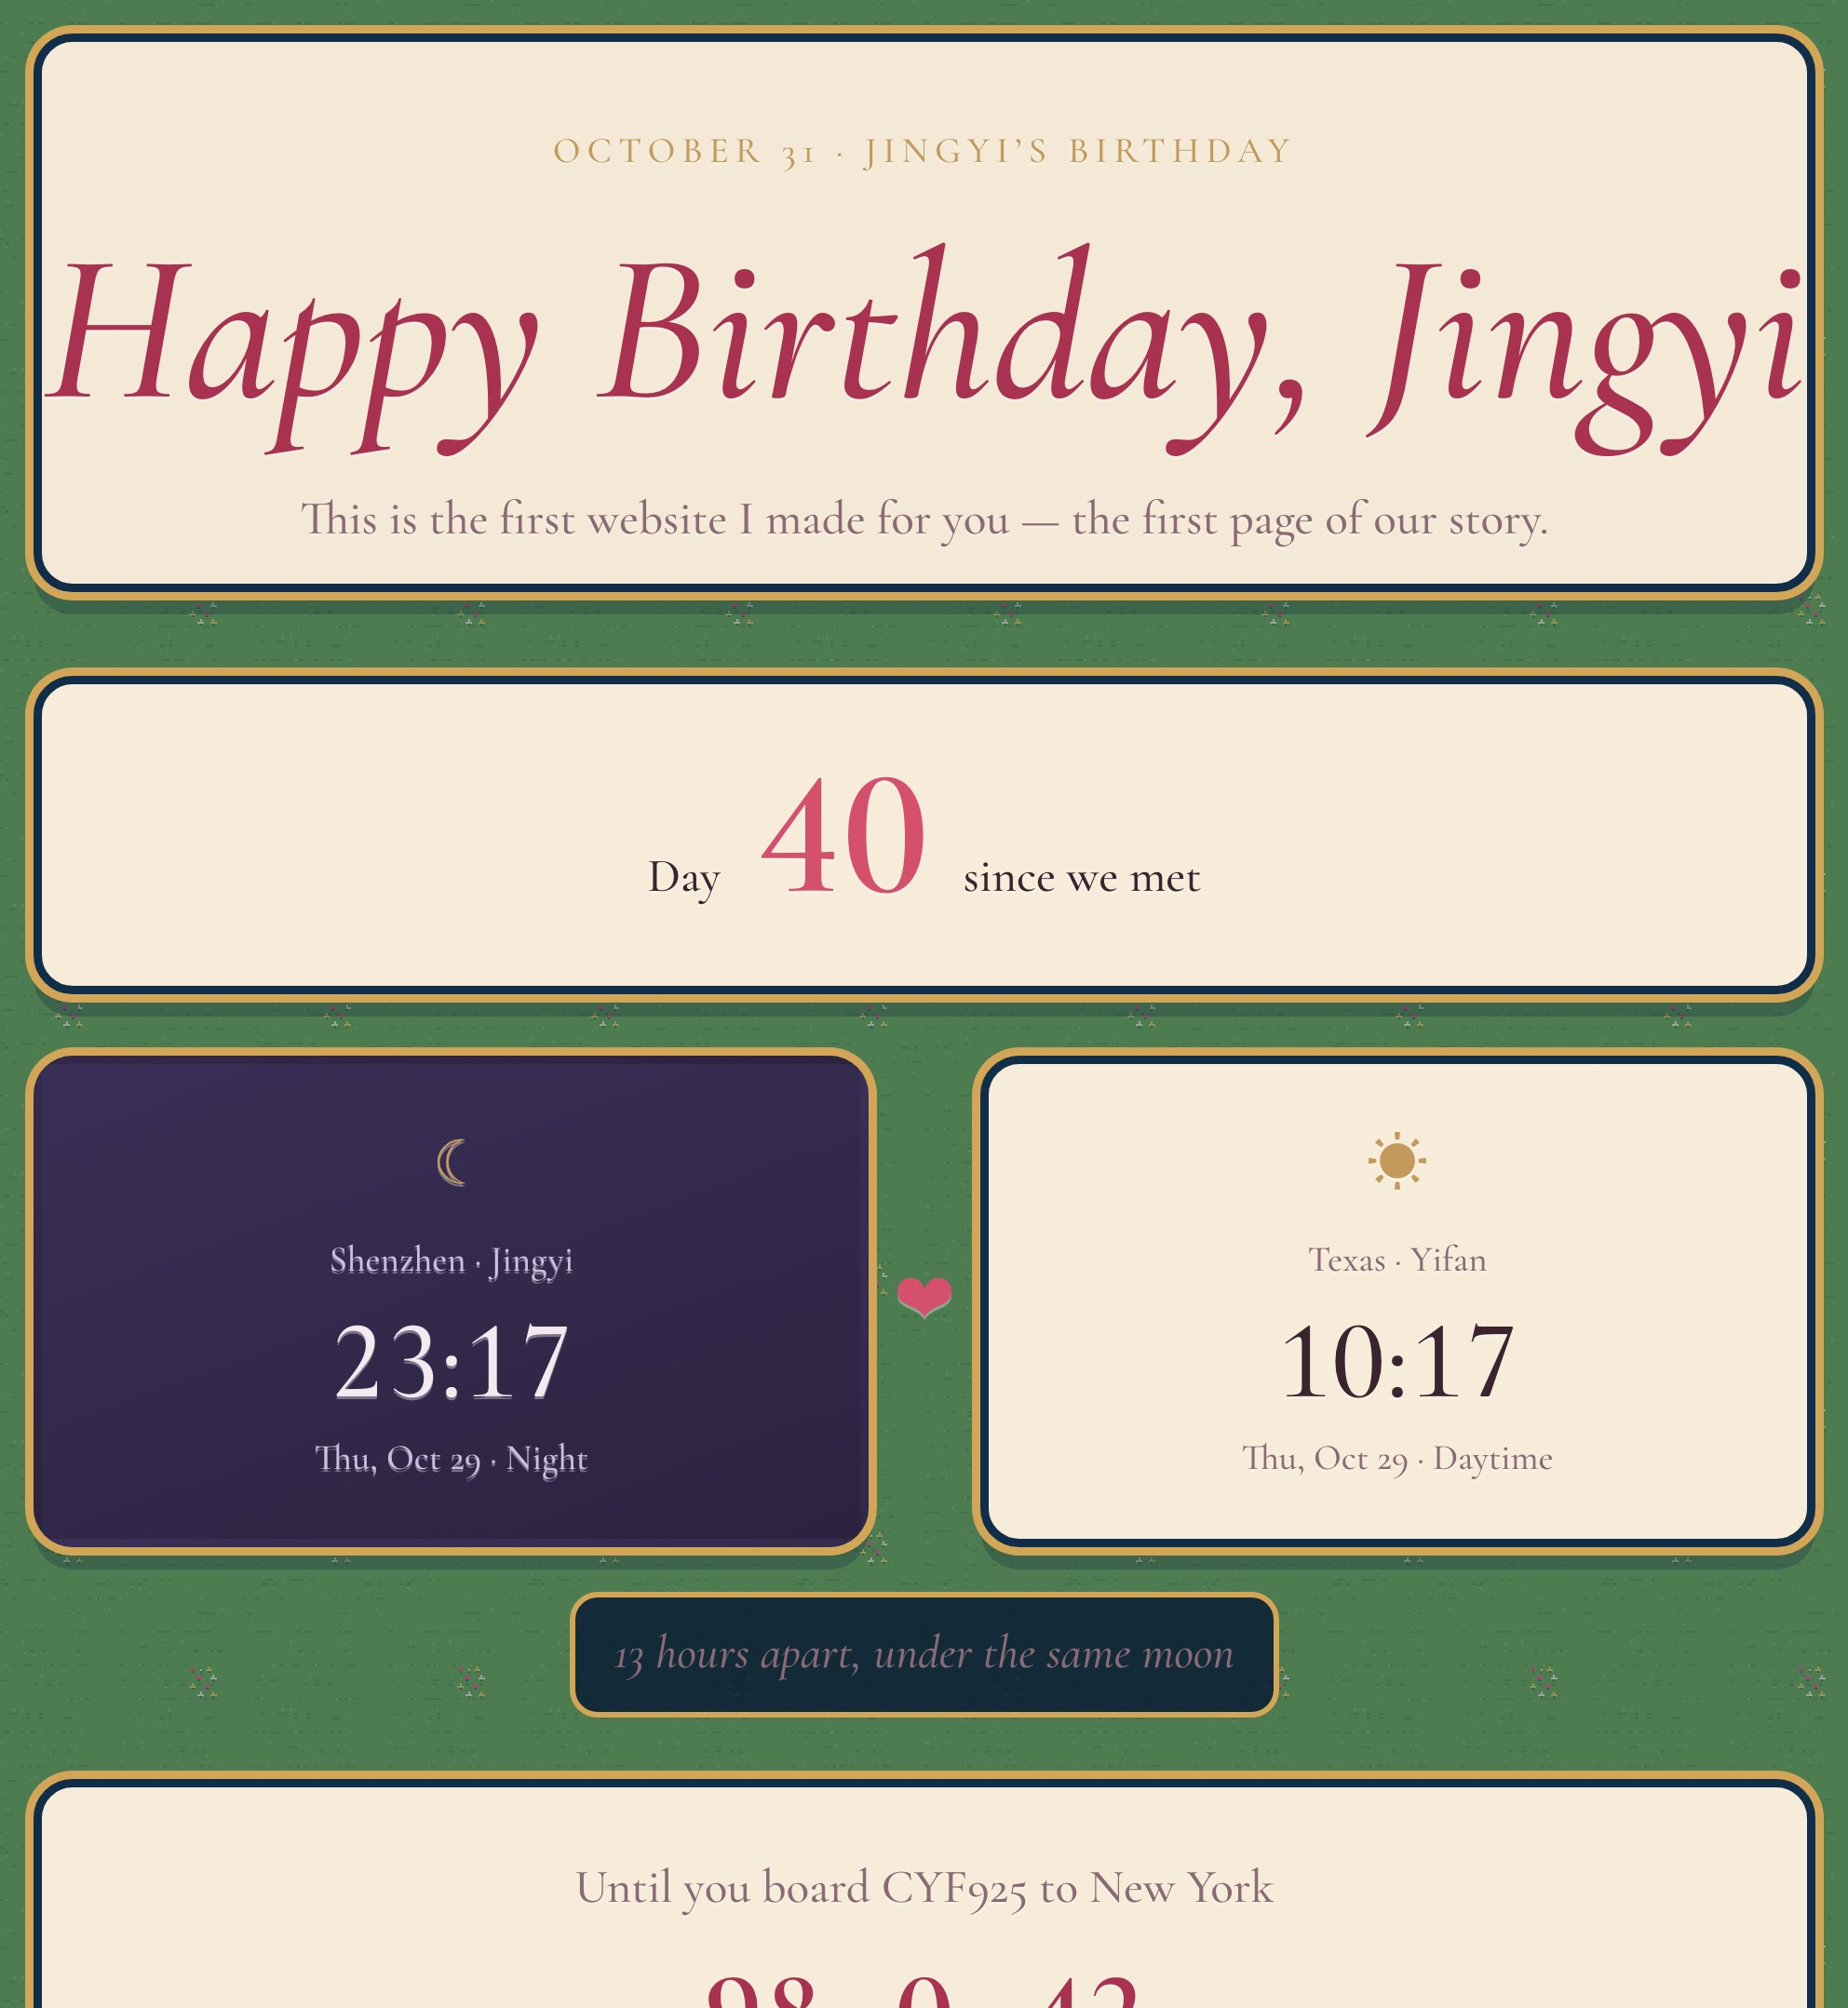
\includegraphics[width=\linewidth]{figures/page-met.jpg}\caption{1 The Day We Met}\end{subfigure}\hfill
  \begin{subfigure}[b]{0.24\textwidth}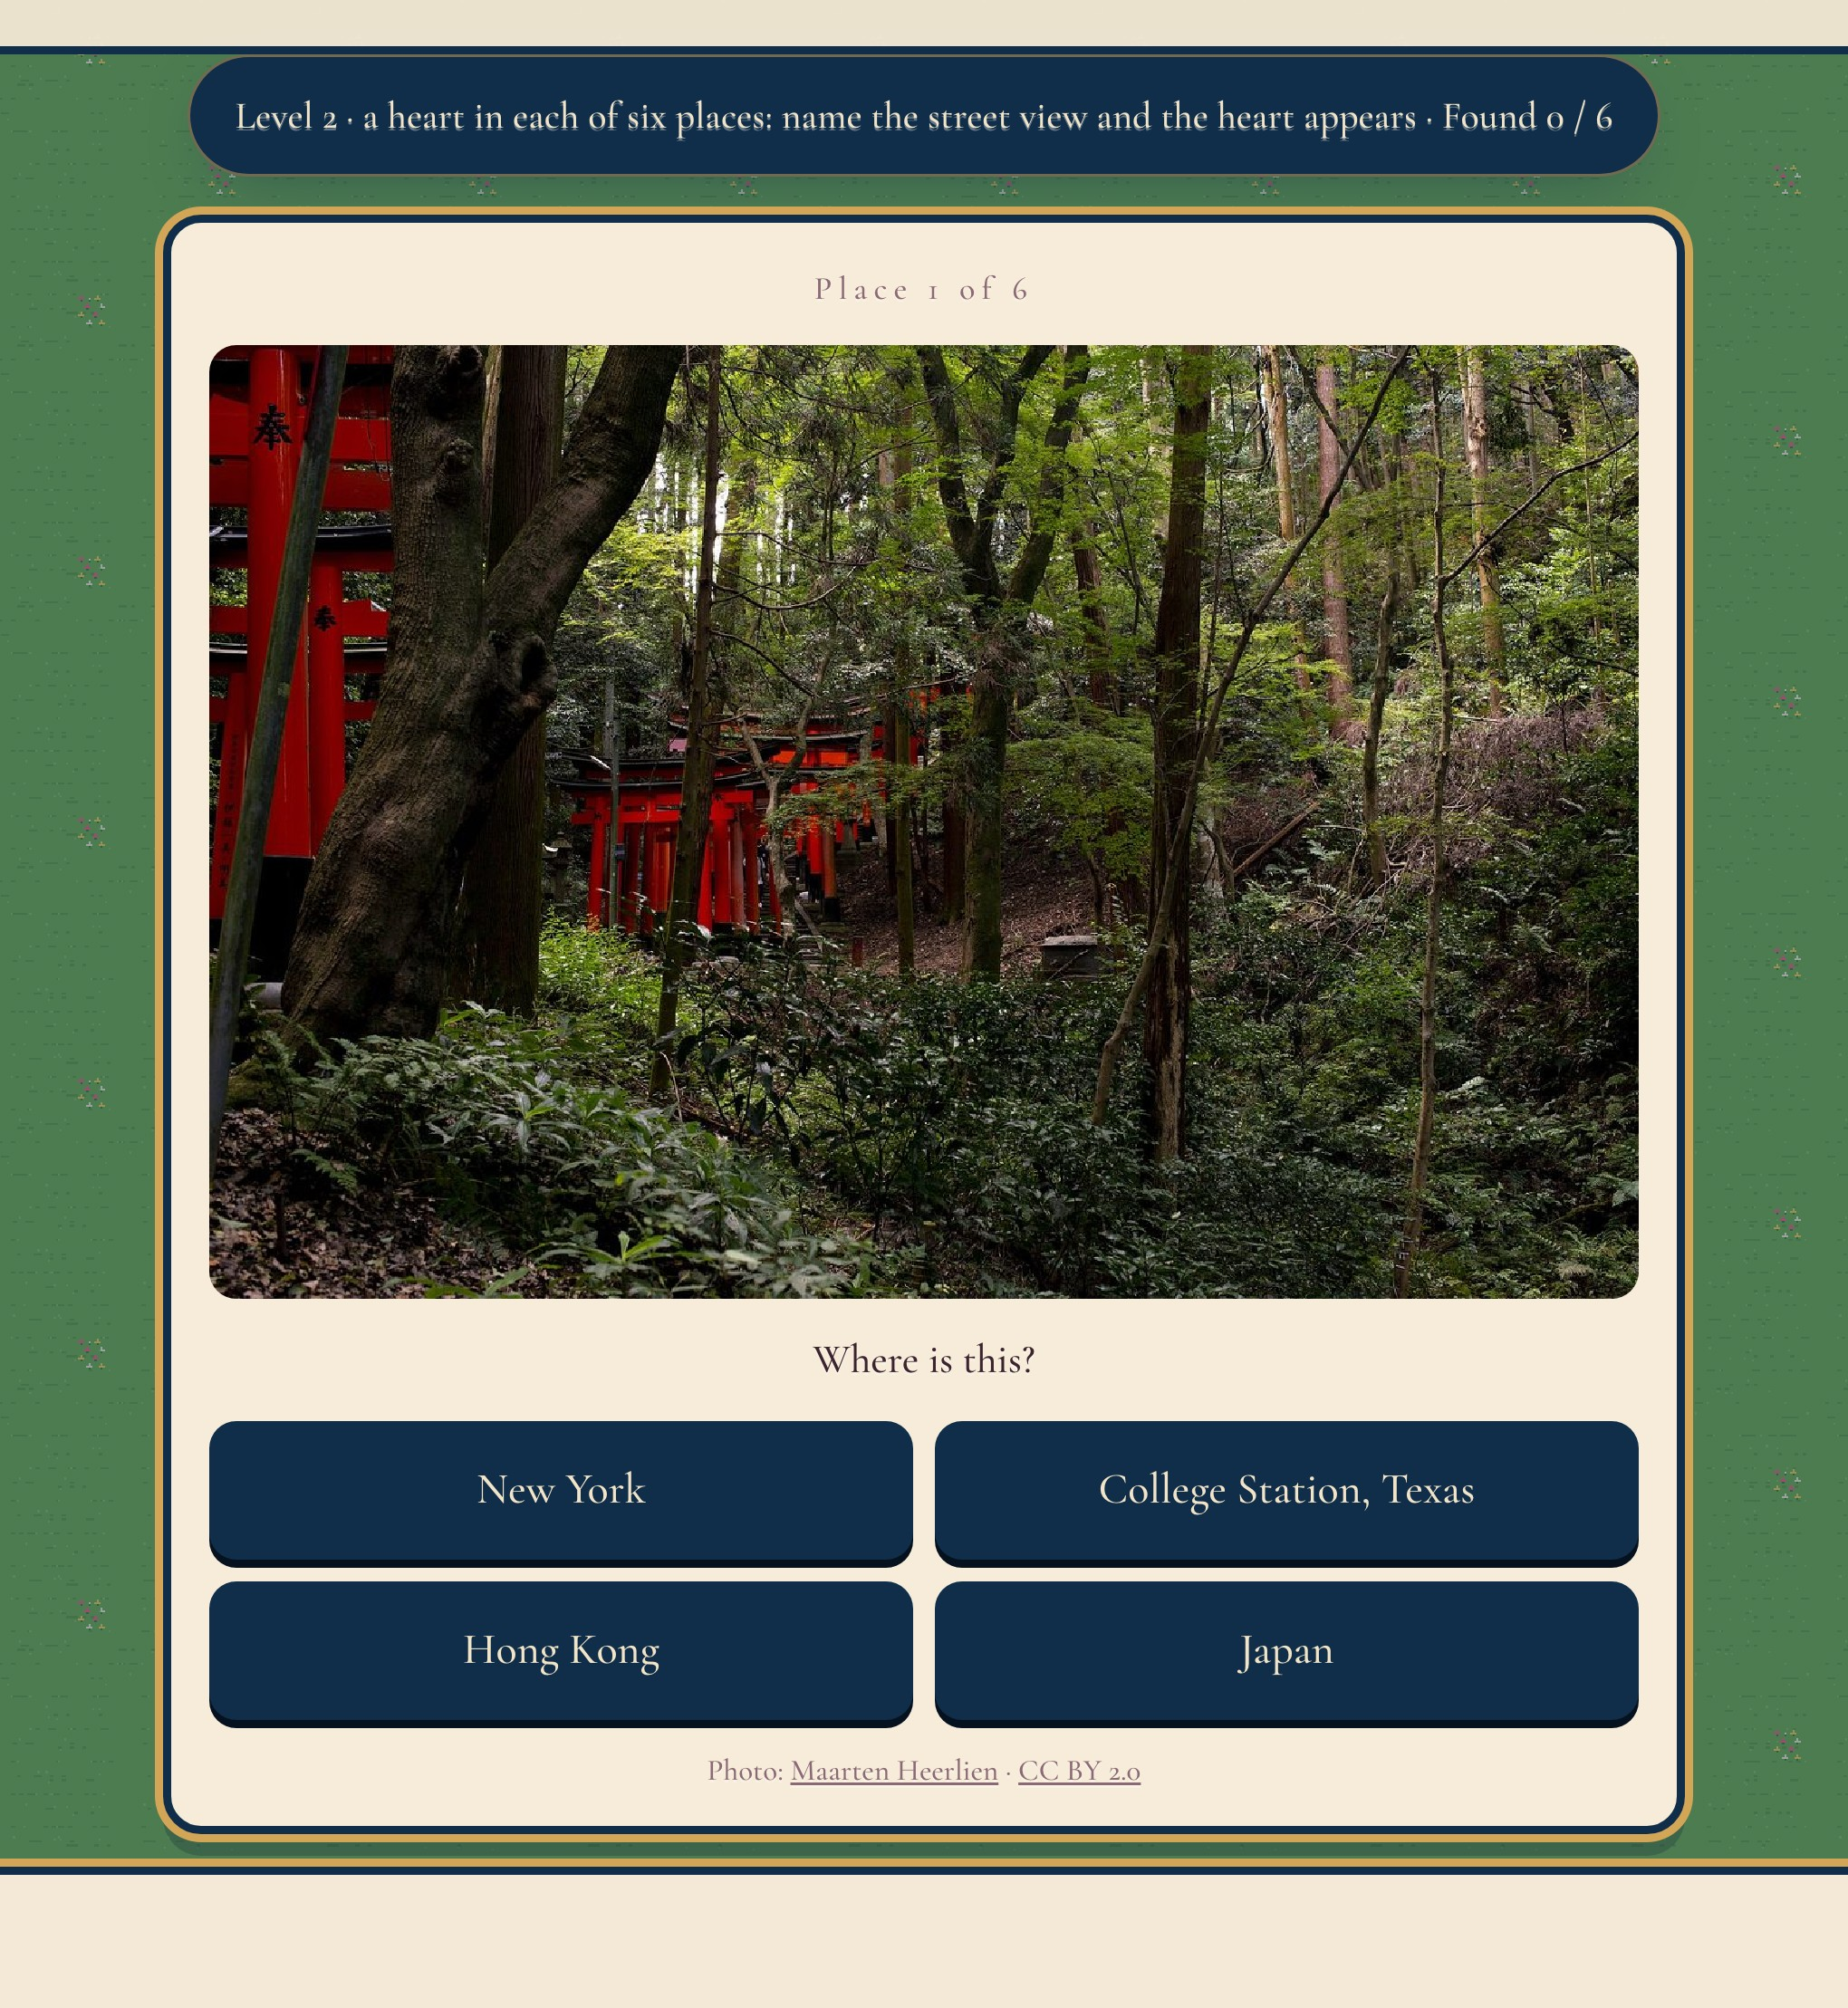
\includegraphics[width=\linewidth]{figures/page-map.jpg}\caption{2 Love Map}\end{subfigure}\hfill
  \begin{subfigure}[b]{0.24\textwidth}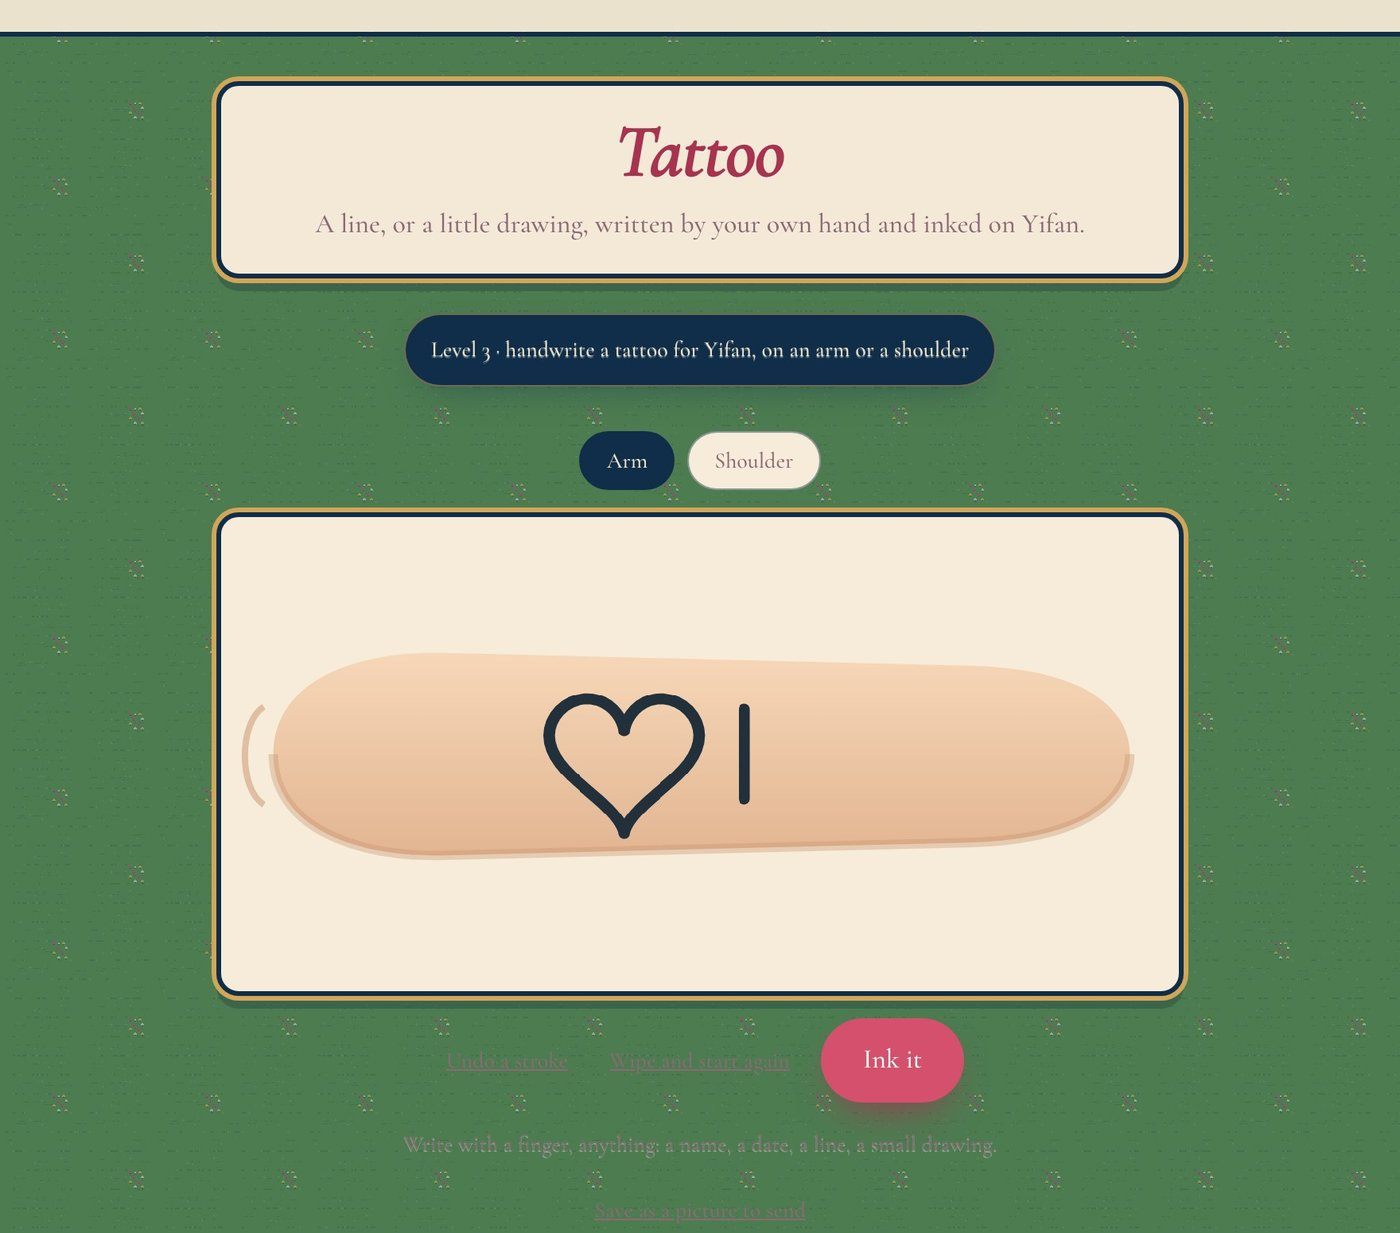
\includegraphics[width=\linewidth]{figures/page-tattoo.jpg}\caption{3 Tattoo}\end{subfigure}\hfill
  \begin{subfigure}[b]{0.24\textwidth}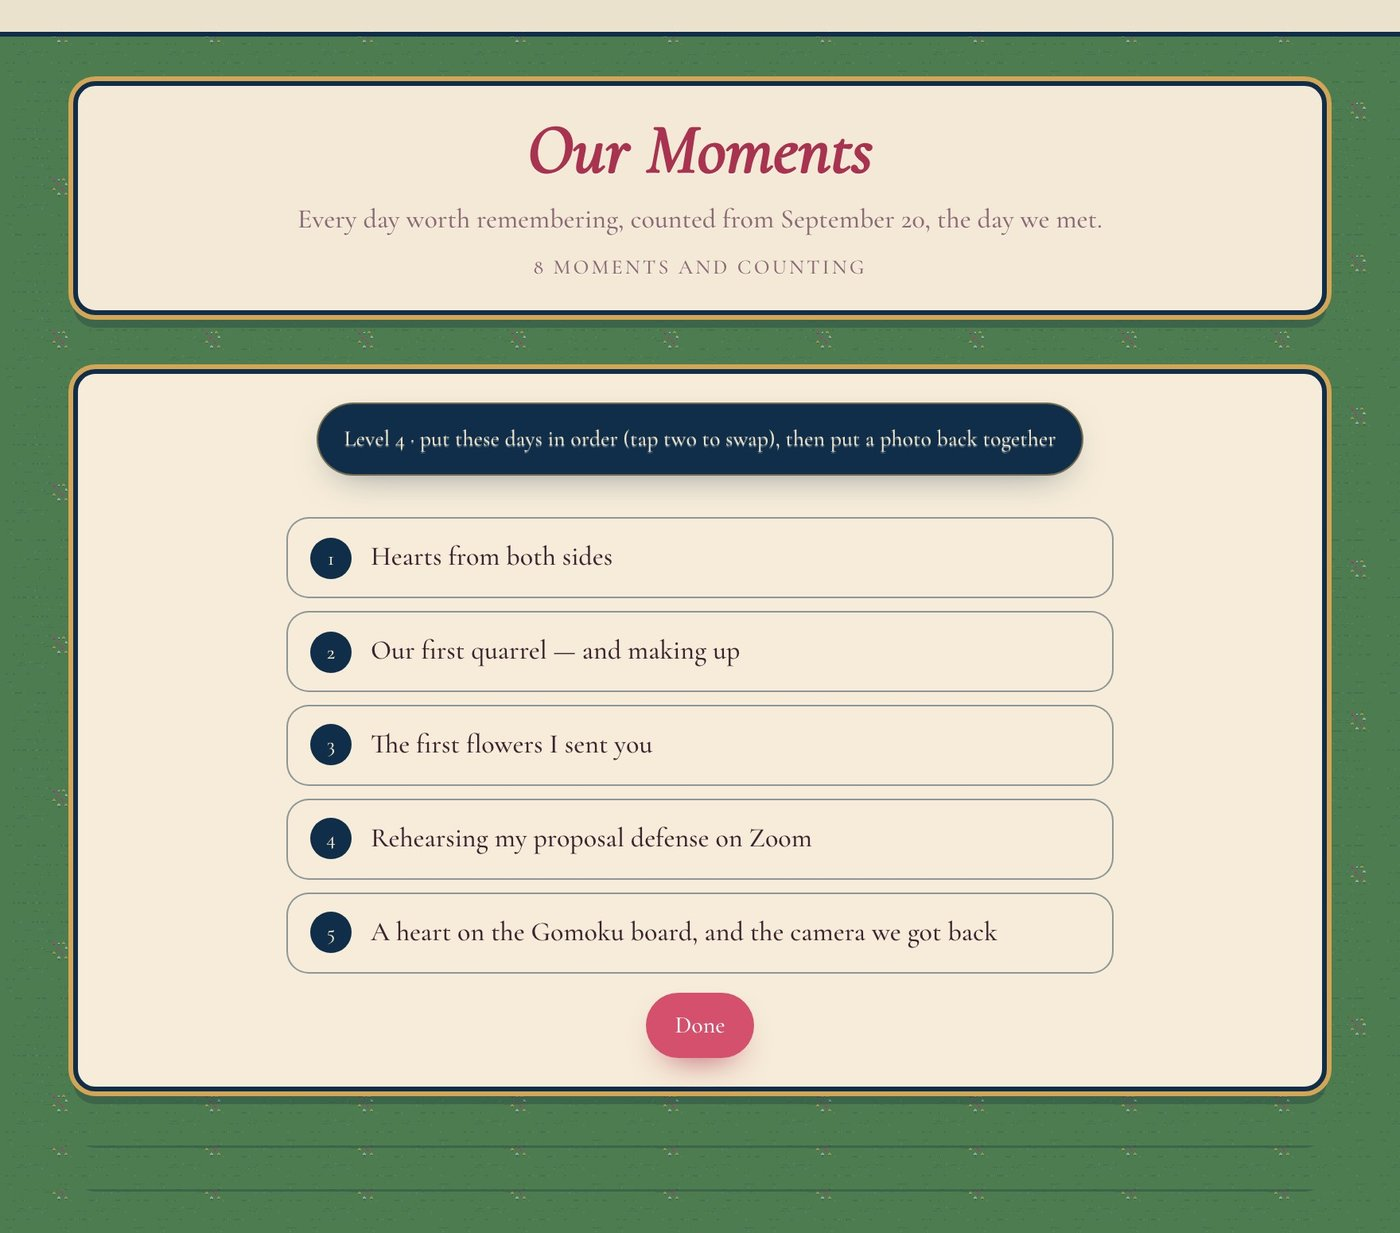
\includegraphics[width=\linewidth]{figures/page-moments.jpg}\caption{4 Moments}\end{subfigure}\\[4pt]
  \begin{subfigure}[b]{0.24\textwidth}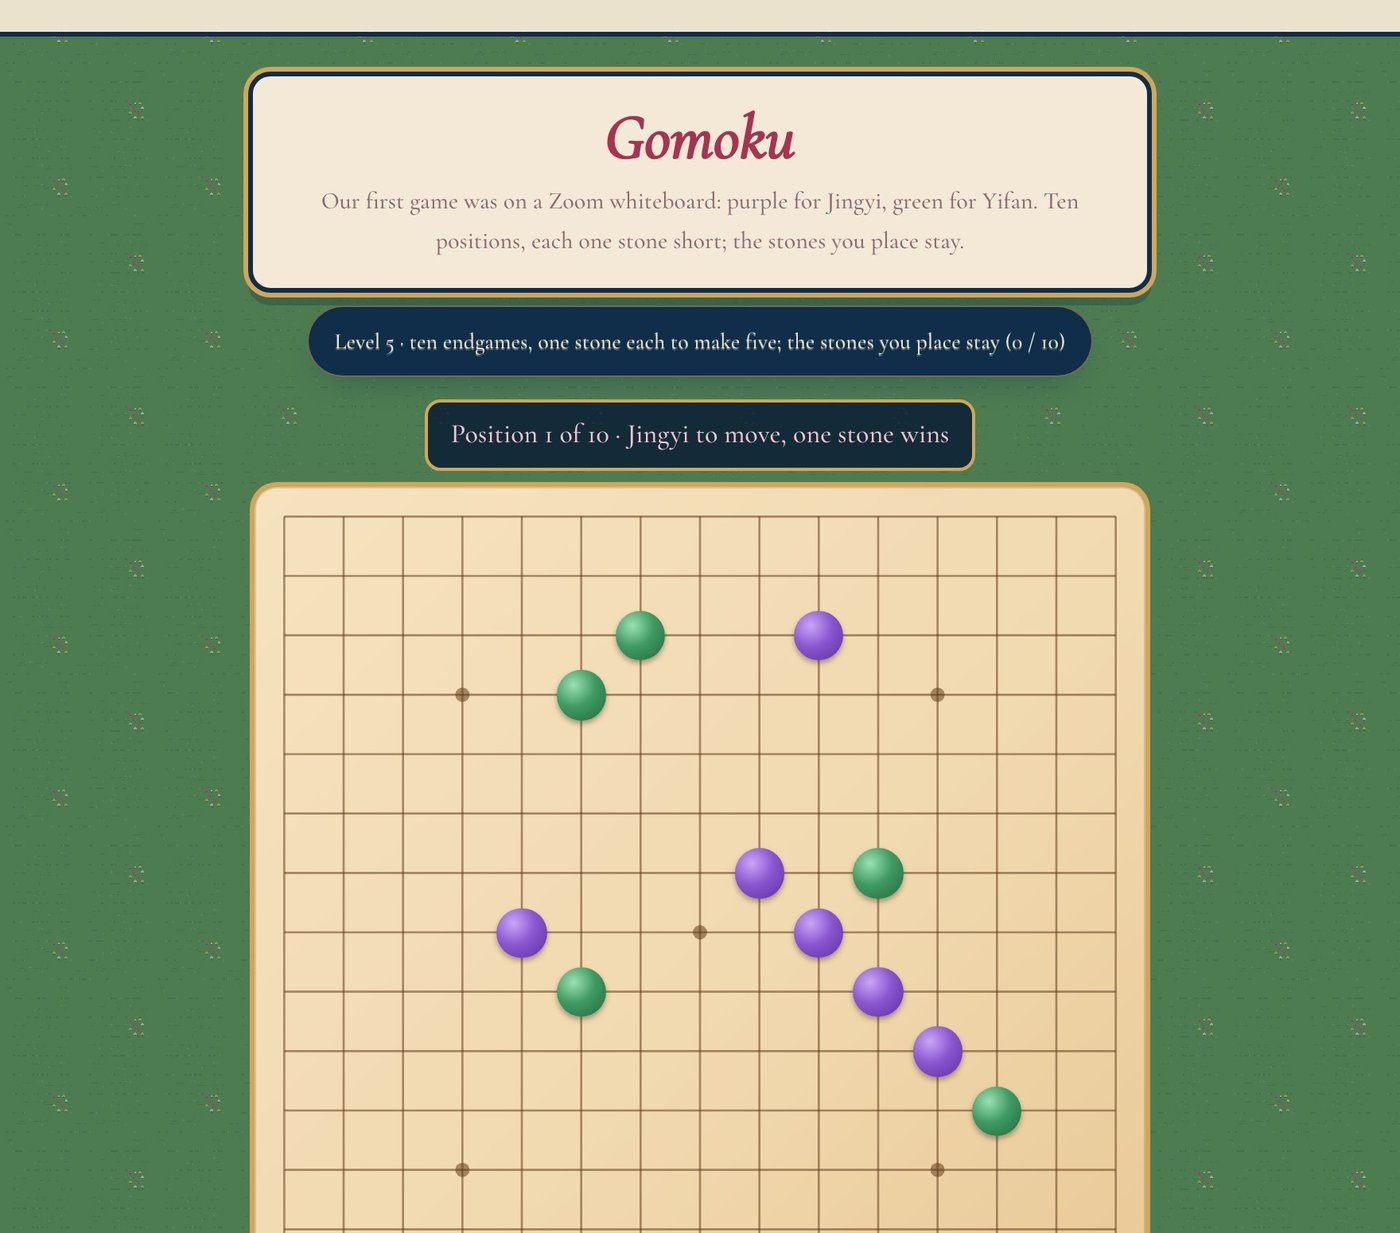
\includegraphics[width=\linewidth]{figures/page-gomoku.jpg}\caption{5 Gomoku}\end{subfigure}\hfill
  \begin{subfigure}[b]{0.24\textwidth}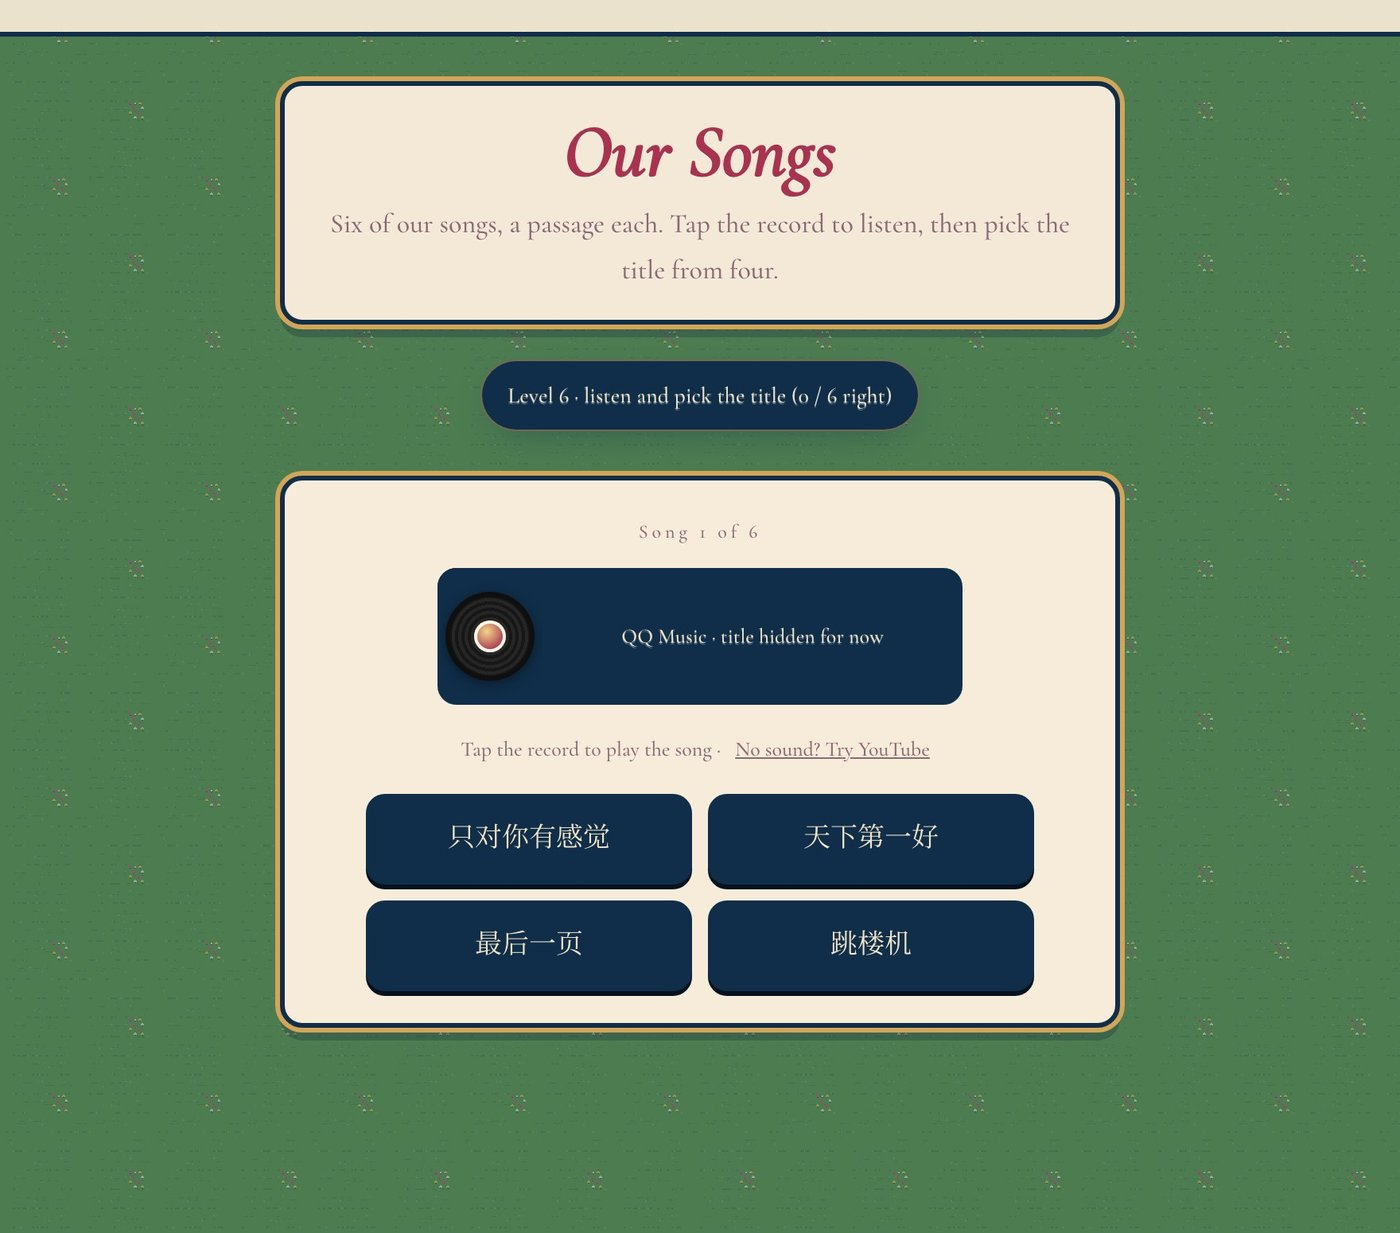
\includegraphics[width=\linewidth]{figures/page-songs.jpg}\caption{6 Our Songs}\end{subfigure}\hfill
  \begin{subfigure}[b]{0.24\textwidth}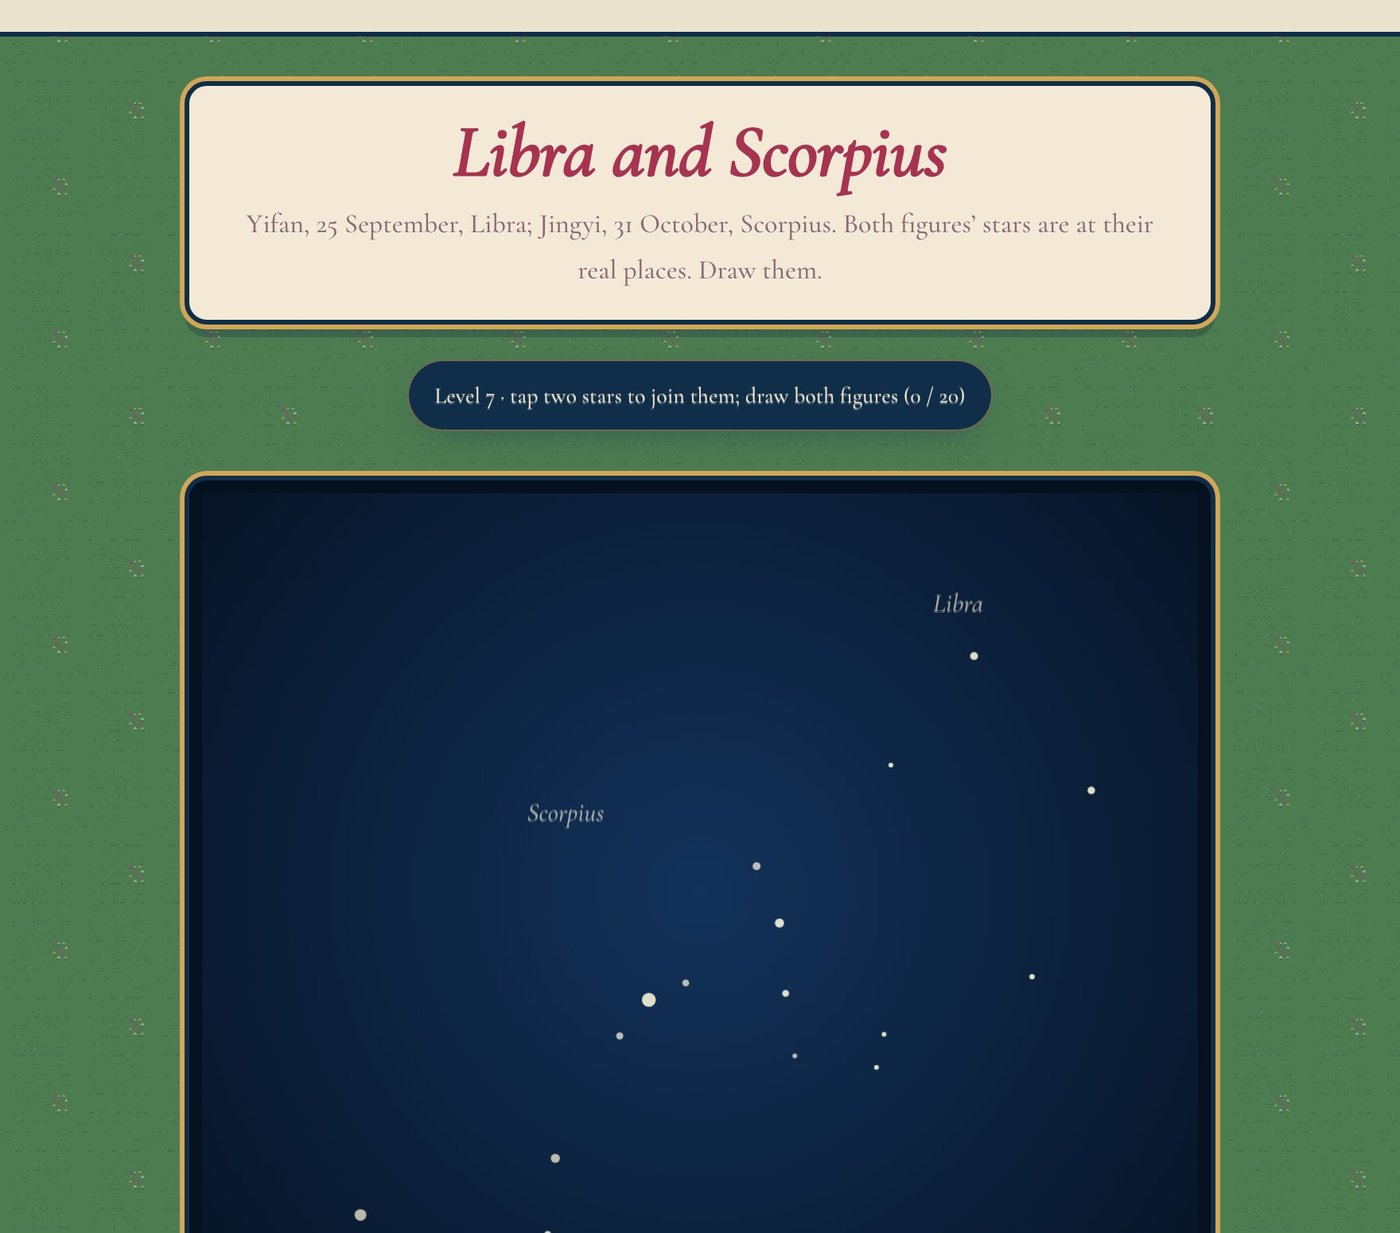
\includegraphics[width=\linewidth]{figures/page-stars.jpg}\caption{7 Libra and Scorpius}\end{subfigure}\hfill
  \begin{subfigure}[b]{0.24\textwidth}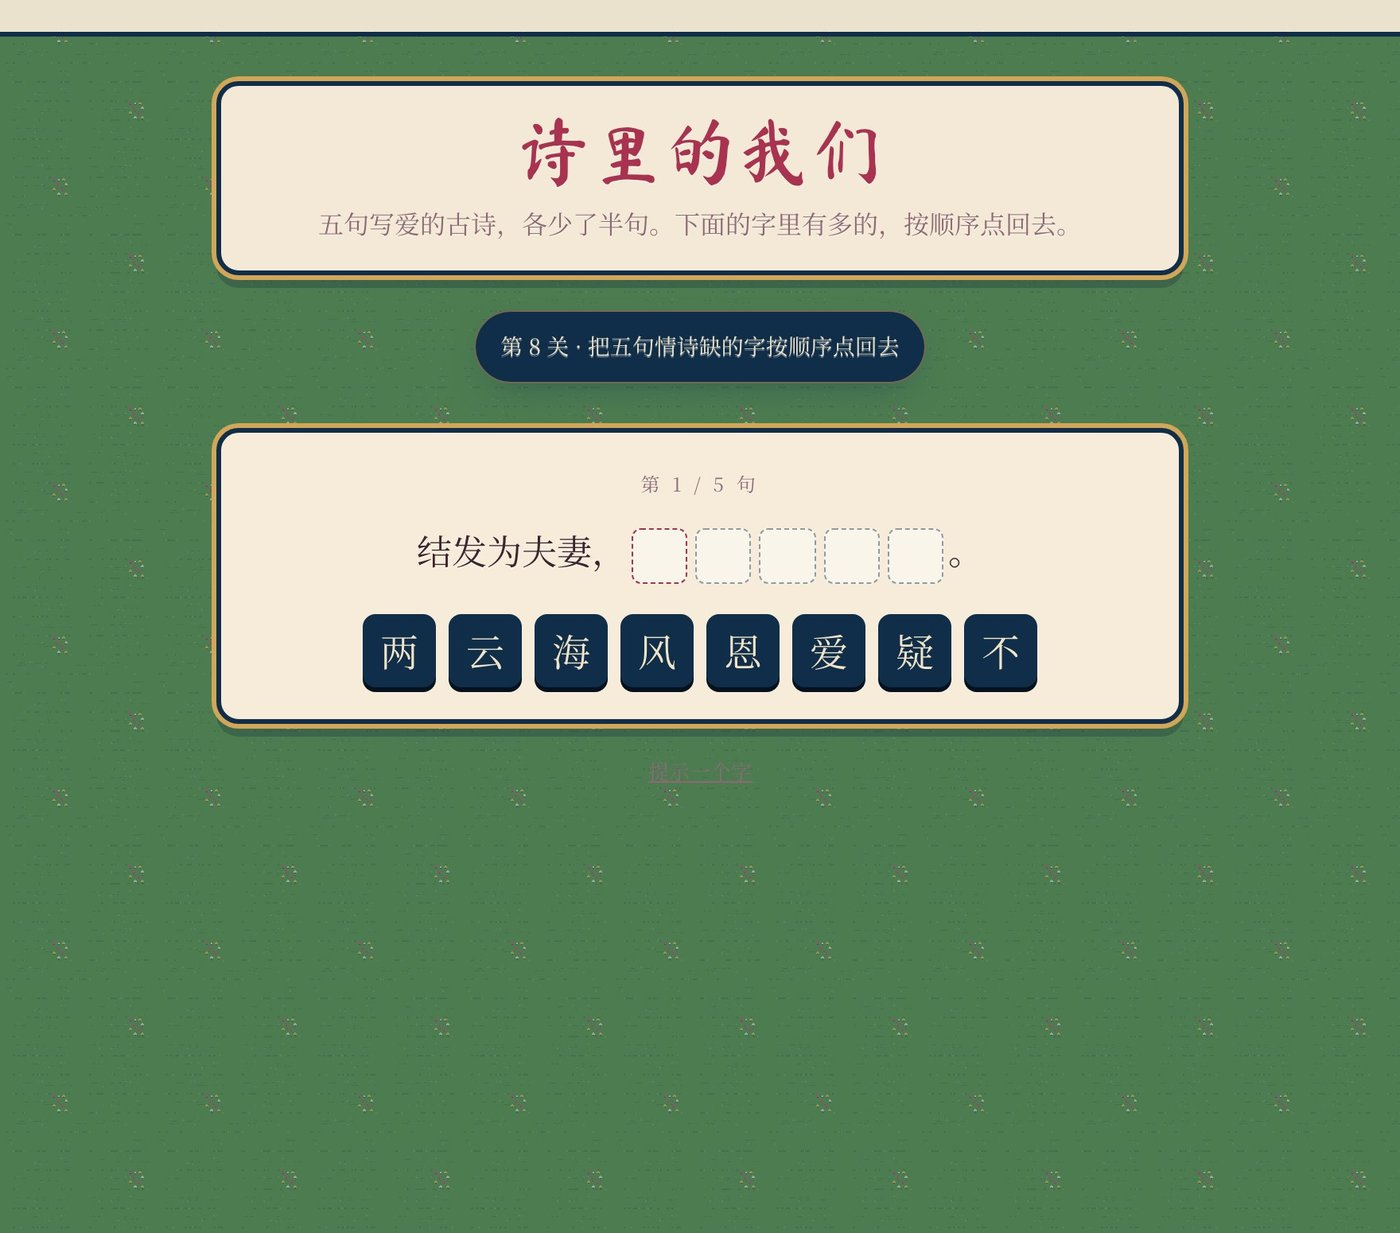
\includegraphics[width=\linewidth]{figures/page-poems.jpg}\caption{8 Us, in Old Verse}\end{subfigure}
  \caption{Eight of the nine levels in play (the ninth is shown in Figure~\ref{fig:ring}). (a) Day
  counter, twin clocks and the countdown to CYF925. (b) Name the place in the street view (photograph: Maarten Heerlien, CC~BY~2.0, via Wikimedia Commons). (c)~A
  heart inked on an arm. (d) Put the first days in order (the photographs below are omitted here). (e) Position~1 of~10: one stone wins.
  (f)~Name the song. (g) Libra's ``claws'' and Scorpius, before they are joined. (h) A line traditionally attributed to Su Wu,
  \kai{结发为夫妻，恩爱两不疑} with its second half to restore.}
  \Description{Eight screenshots of the levels, each a cream panel on green pixel grass.}
  \label{fig:levels}
\end{figure*}

\paragraph{1. The Day We Met.} The first level shows the day count since 20 September, the time
in both cities with day and night icons, and a countdown to the flight. To clear it, each player
reads a vow, rewritten from the wedding formula as the vow of ``becoming each other's partner
once more'', and says one line aloud: \zh{我爱你，陈静仪，我愿意} (``I love you, Jingyi Chen, I do''),
with the partner's full name. Browser speech recognition~\cite{w3c2023speech} hears Mandarin
names inconsistently, so the matcher removes everything except Han characters and Latin
letters and accepts any of eight or nine homophone spellings of each name (for example \zh{陈静怡},
\zh{陈静宜}). A typed fallback keeps the level playable in browsers that cannot listen.

\paragraph{2. Love Map.} Six places matter to the couple: Texas, Los Angeles, Japan, Shenzhen,
Hong Kong and New York. The street views are public photographs of well-known sites from
Wikimedia Commons rather than the couple's own pictures, since a personal photograph can give away
far more of a place than its owner intends~\cite{yang2024geolocator}. Before each heart appears on a Leaflet map, the player names a
street-level photograph from four options (Figure~\ref{fig:levels}b), and a wrong pick reshuffles the
options. Great-circle arcs connect the two home cities.

\paragraph{3. Tattoo.} The player handwrites a line or a small drawing on an arm or a shoulder,
drawn in SVG, and inks it. The tattoo is kept on the device and can be saved as an image to send.

\paragraph{4. Moments.} The timeline holds eight dated memories, each with photos and a story in
both languages, from hearts made from both sides of the ocean (day~21) to a heart drawn on the
Gomoku board (day~35). The player orders five of them by tapping pairs to swap, then reassembles a
$3\times3$ portrait of the partner.

\paragraph{5. Gomoku.} Each of ten positions on a $15\times15$ board has exactly one winning point
for the player's own colour (purple for Jingyi, green for Yifan, as in their first game). The ten
answers are the ten points of a heart; solved answers stay on the board in gold, so the heart draws
itself as the player progresses. Positions are generated from three patterns (a four closed at one
end, a broken four, three-and-one) placed around each heart point in varied directions with decoy
stones, and a test checks that each has a unique winning move. Gomoku is a first-player win under
optimal play~\cite{allis1994searching}; win-in-one puzzles avoid that question entirely and make
every move feel like a find.

\paragraph{6. Our Songs.} Six songs the couple share (among them \zh{只对你有感觉} and
\zh{天下第一好}) play a passage through the official embedded players: QQ Music for the player in
China and YouTube for the player in the United States, each switchable. The site hosts no audio.
For embedded players, the options unlock after eight seconds on screen because playback
events are unavailable. This delay does not verify that a passage was heard.

\paragraph{7. Libra and Scorpius.} Yifan is a Libra (25 September) and Jingyi a Scorpio
(31 October); in the sky the two constellations are neighbours, and Libra's two brightest stars
still bear the Arabic names of the Scorpion's claws, \emph{Zubenelgenubi} and
\emph{Zubeneschamali}. The level projects 21 manually entered stars, six for Libra and fifteen for Scorpius,
and asks the player to draw 20 edges. The source records coordinates as J2000 right ascension
and declination; Meeus provides astronomical coordinate conventions~\cite{meeus1998astronomical},
not provenance for these particular star entries. The chart is an illustration, not a computed
view of either player's current night sky.

\paragraph{8. Us, in Old Verse.} Five classical lines about love lose their second half, to be
restored from a bank of characters: a farewell traditionally attributed to Su Wu, \kai{结发为夫妻，恩爱两不疑};
Guan Daosheng's \emph{Song of You and Me}; a couplet of Li Shangyin; the paired birds of the
sixth-century anthology \emph{New Songs from a Jade Terrace}~\cite{birrell1982jade}; and an
anonymous couplet. Each solved line shows a plain English gloss.

\paragraph{9. Meridian.} The last level is a pair of rings, called \emph{Meridian}, modelled
procedurally in Blender from a Python script (Figure~\ref{fig:ring}). The pair share a signature:
a yellow-gold line inlaid around a platinum band like a meridian on a globe, a hidden sapphire
inside the bottom, and an inner engraving that carries the \emph{other} person's name and birthday,
the date they met and the coordinates of the airport where they will meet ($40.64^\circ$N
$73.78^\circ$W). Her ring exists in two designs, a solitaire on four compass prongs (v1) and the
current flush-set stone sunk into his band's profile (v2); the page keeps both as a design history.
The level is cleared only one way: the player tries the ring on through the camera and takes a
photo (Section~\ref{sec:sensing}).

\begin{figure}[t]
  \centering
  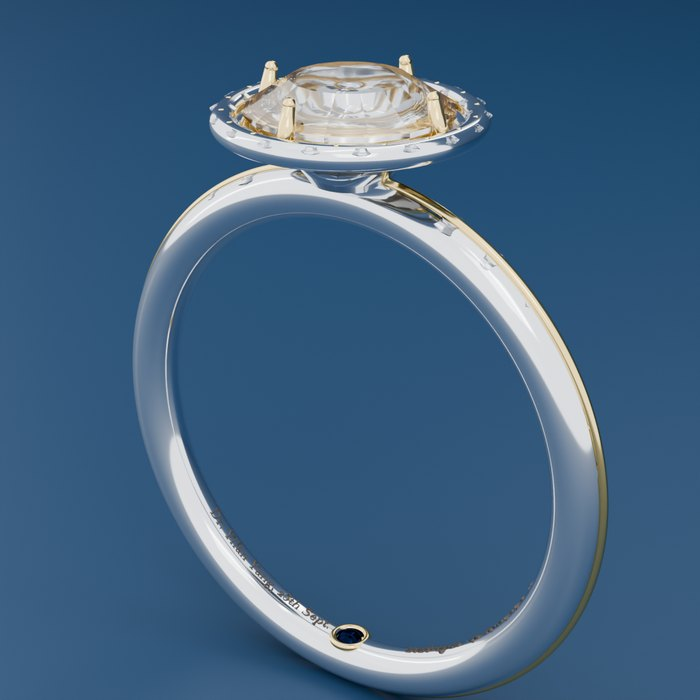
\includegraphics[width=0.325\columnwidth]{figures/hers_v1_hero.jpg}\hfill
  
\includegraphics[width=0.325\columnwidth]{figures/hers_hero.jpg}\hfill
  
\includegraphics[width=0.325\columnwidth]{figures/his_hero.jpg}
  \caption{The Meridian pair, path-traced from the procedural Blender model: hers v1 (solitaire,
  halo and graduated shoulder stones), hers v2 (flush-set 4.2\,mm stone in a 5\,mm flat band), and
  his (brushed flat comfort-fit band). The gold meridian runs around each band.}
  \Description{Three renders of rings on a dark background: a diamond solitaire, a flat band with
  a sunken stone, and a plain wide band, each with a thin gold line around it.}
  \label{fig:ring}
\end{figure}

\subsection{Two Days}\label{sec:days}
Two signposts lead from the square to a day in each city (Figure~\ref{fig:days}). Each is a second
map with the person's stops: Yifan's home, gym, his advisor's office, the golf course and the
pool in College Station; Jingyi's home with the cats at the door, her drive, the office and
Shenzhen Bay. Each stop has hours, and the person's sprite stands wherever the clock in their own
city puts them. A partner who opens Yifan's day at 9:49 p.m. in Shenzhen finds him at 8:49 a.m. at
his advisor's office. These are authored schedules, not live location tracking. They began as guesses and were corrected by the designer: Yifan drives
rather than taking the bus; Jingyi drives a Tesla rather than taking the metro; and the
Shenzhen Bay stop keeps a joke between them about where they will one day live.

\begin{figure}[t]
  \centering
  \begin{subfigure}[b]{0.49\columnwidth}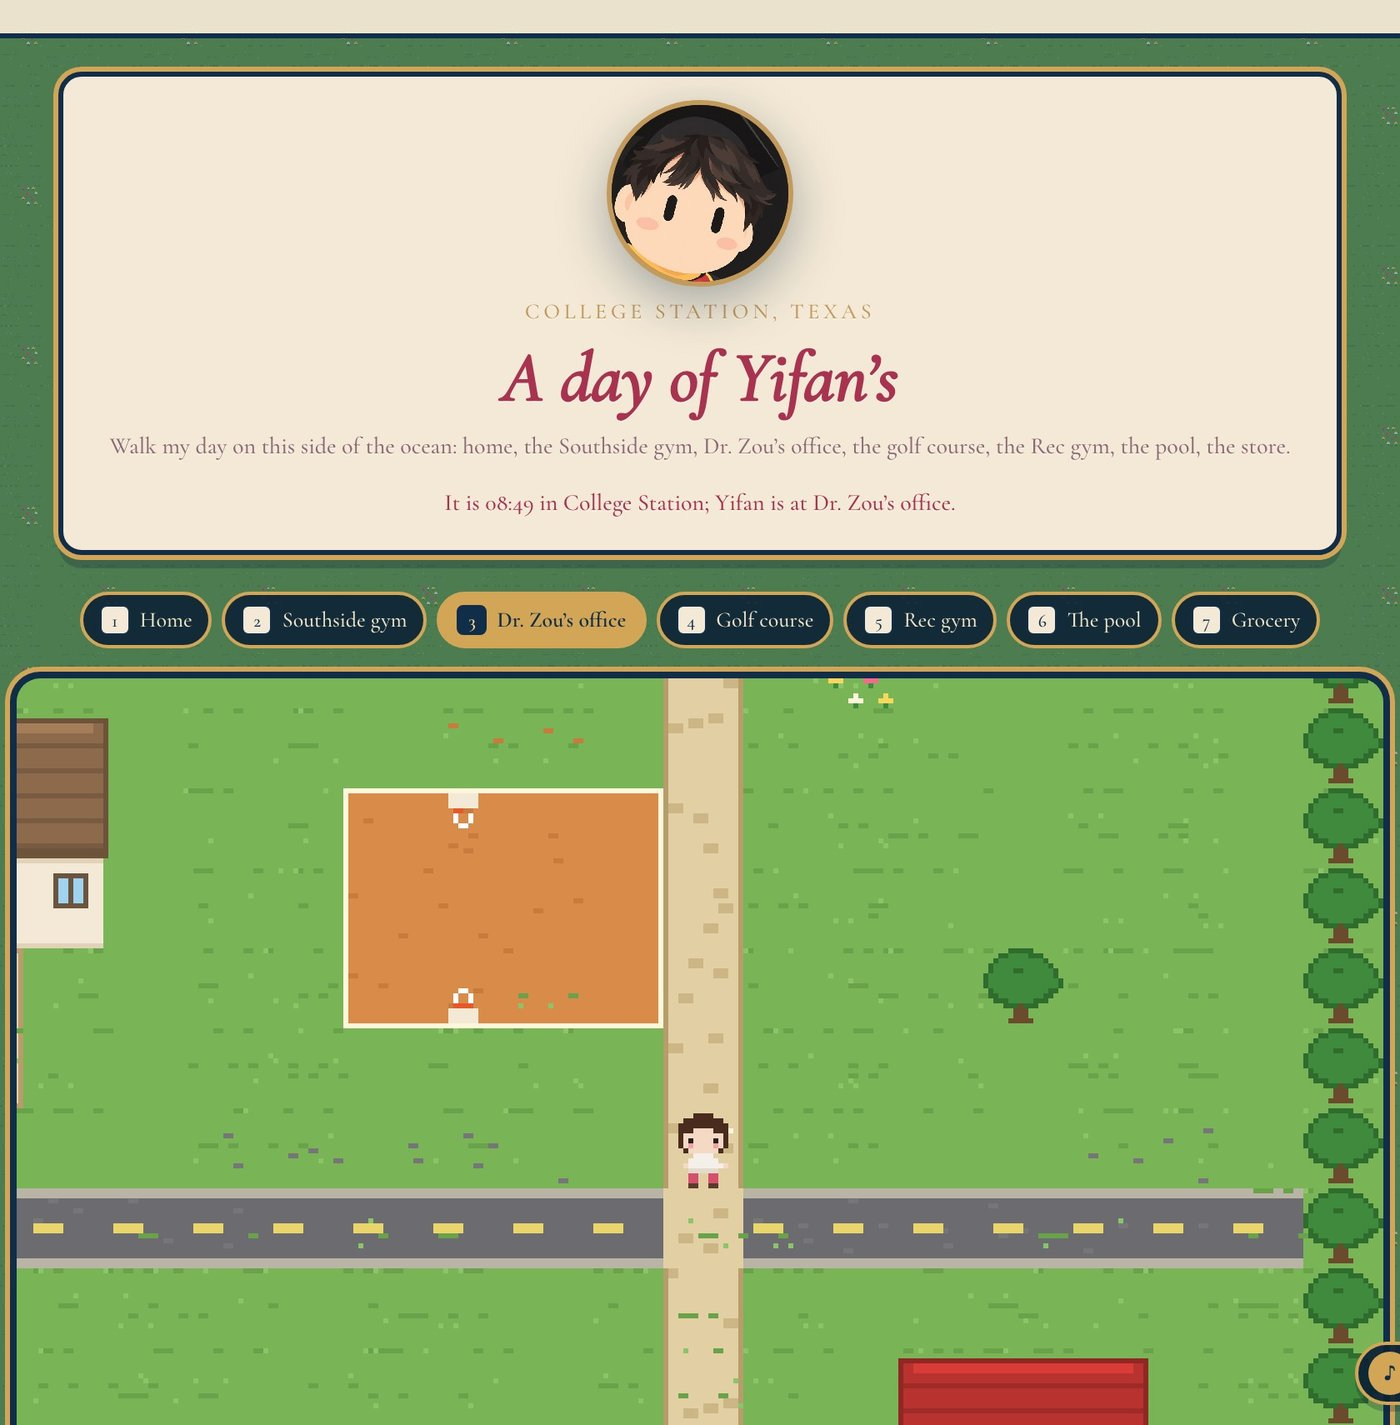
\includegraphics[width=\linewidth]{figures/page-cs.jpg}\caption{A day of Yifan's}\end{subfigure}\hfill
  \begin{subfigure}[b]{0.49\columnwidth}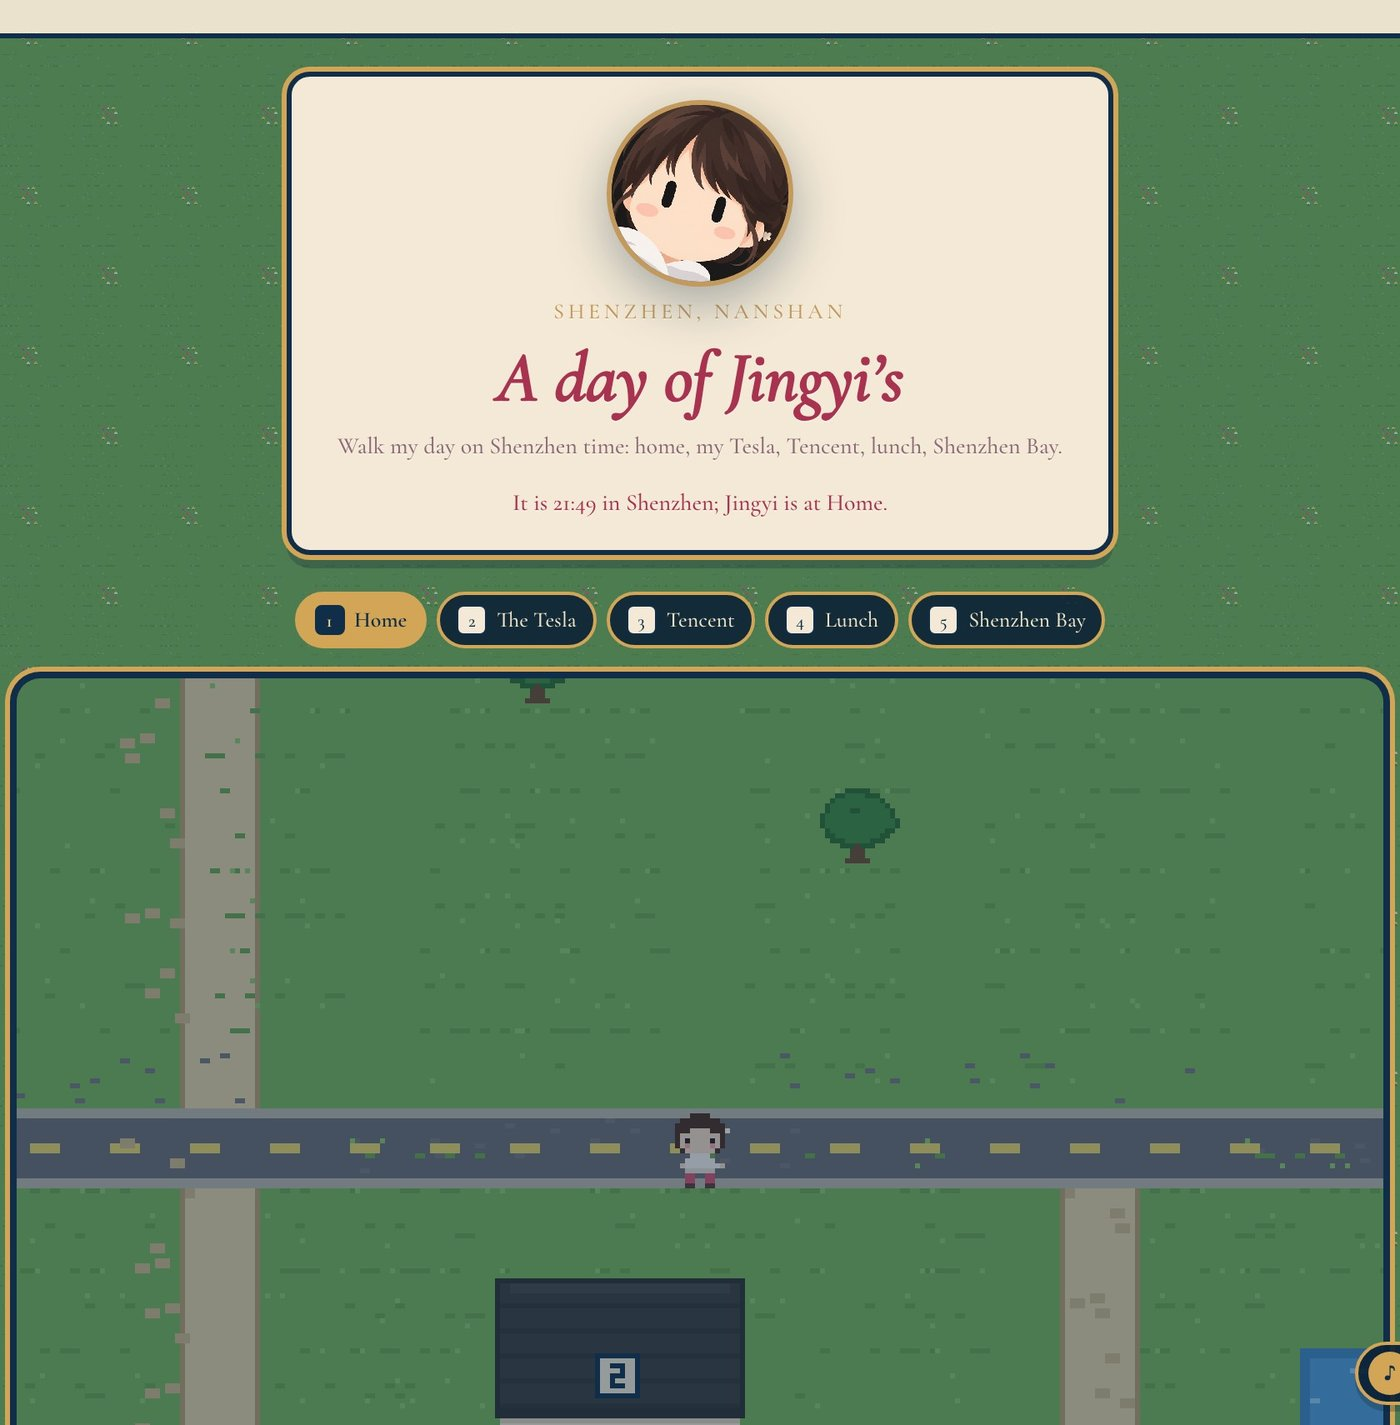
\includegraphics[width=\linewidth]{figures/page-sz.jpg}\caption{A day of Jingyi's}\end{subfigure}
  \caption{The two cities as maps. The person stands at the stop whose hours contain the current
  local time in their own city: (a) Yifan at his advisor's office at 8:49 a.m.\ in College
  Station; (b) Jingyi at home at 9:49 p.m.\ in Shenzhen, the same instant.}
  \Description{Two pixel maps with roads and buildings, each with a person card above it and a row
  of stop buttons.}
  \label{fig:days}
\end{figure}

\subsection{Prologue and Finale}
Two cutscenes frame the game (Figure~\ref{fig:cutscenes}). They run in a small pixel theatre: a
$128\times80$ canvas scaled without smoothing, actors built from the town's sprite sheets, a
darkness layer with candle-like glows, particles, a synthesised score, and a caption box for words
and buttons.

\emph{The birthday prologue} plays once per player before the town opens. In College Station it is
9:47 a.m.; in Shenzhen 10:47 p.m., 73 minutes before Jingyi's birthday. Yifan, in a chef's hat,
bakes the cake against the Shenzhen clock. The player helps by whisking the batter (twelve taps),
placing ten strawberries in the same heart that the Gomoku answers make, and watching nine candles
lit (nine levels; in Chinese \zh{九} ``nine'' sounds like \zh{久} ``for a long time''). At the prologue's scripted Shenzhen midnight, rather than a real-time release gate, the lights go out, the door opens on the town (``In Yi Town there is no thirteen-hour
time difference''), everyone sings, the player makes a wish and blows the candles out, by
breathing into the microphone or holding a button.

\emph{The wedding} opens after the last letter, once both players have cleared the last level.
In the fountain garden at dusk, Rayford reveals why he had worn a suit all along: he is the
master of ceremonies. The groom waits under the arch, the bride walks the aisle to Mendelssohn's
\emph{Wedding March}, the scripted sequence asks for both characters' ``I do'' responses, with speech
recognition where supported, Coffee carries the rings down the aisle on a red pillow, the Meridian rings turn in
3D, and the scene ends in a kiss, bells, doves and a certificate to keep
(Figure~\ref{fig:cert}). Afterwards the town dresses the two sprites as bride and groom.

\begin{figure*}[t]
  \centering
  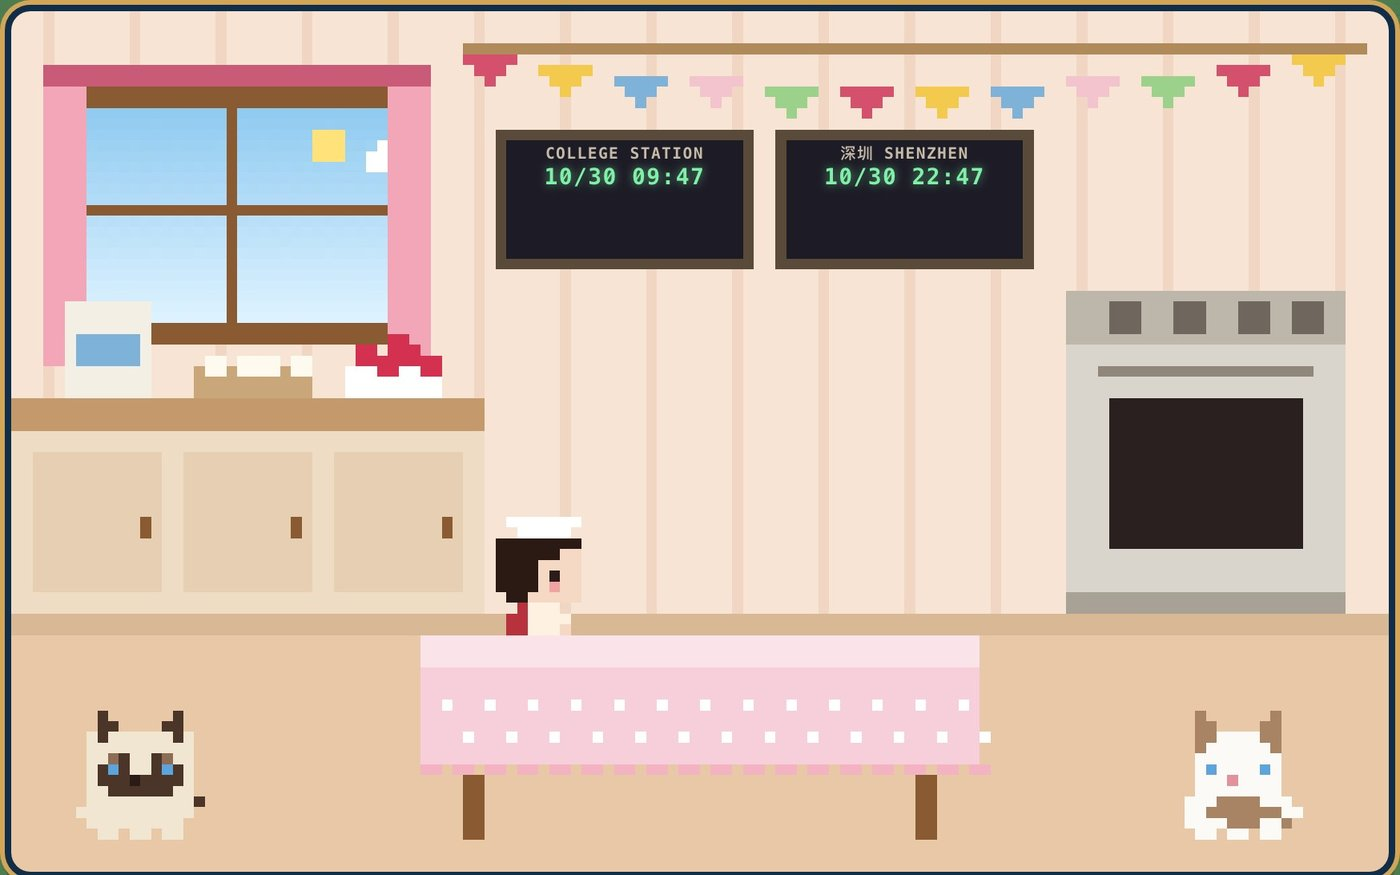
\includegraphics[width=0.245\textwidth]{figures/bday-03.jpg}\hfill
  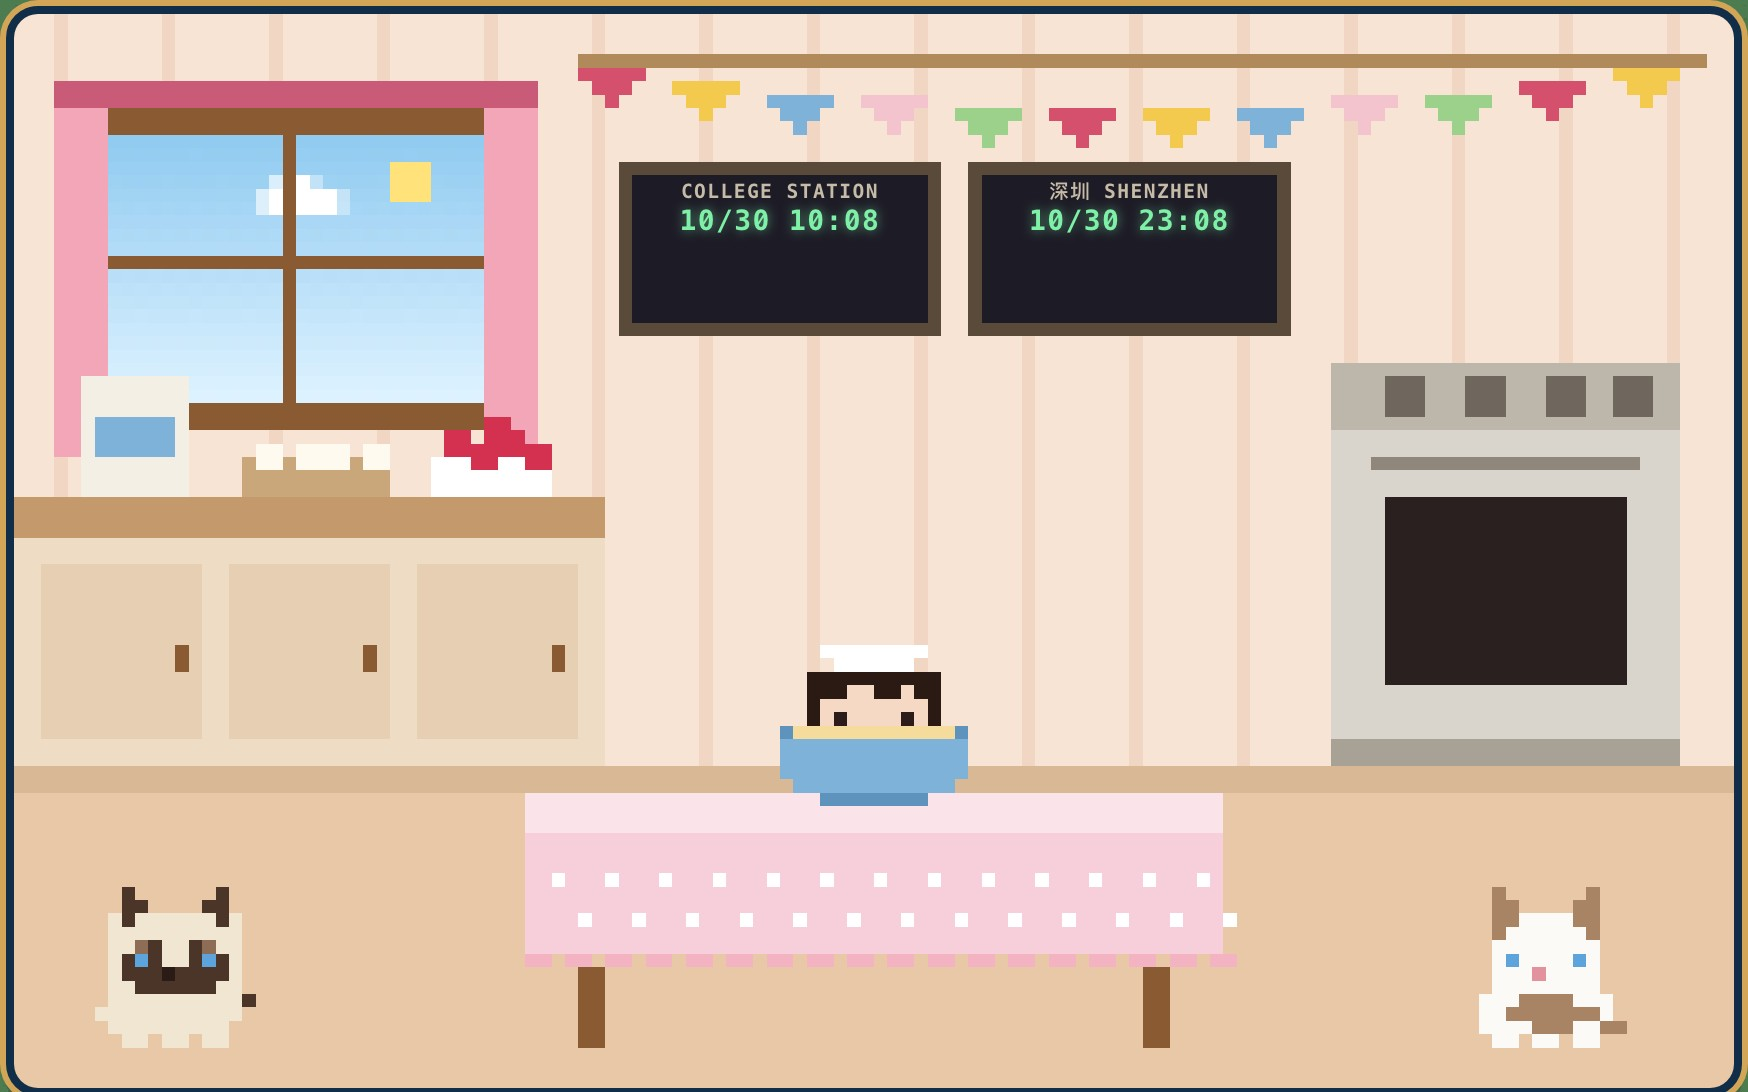
\includegraphics[width=0.245\textwidth]{figures/bday-09.jpg}\hfill
  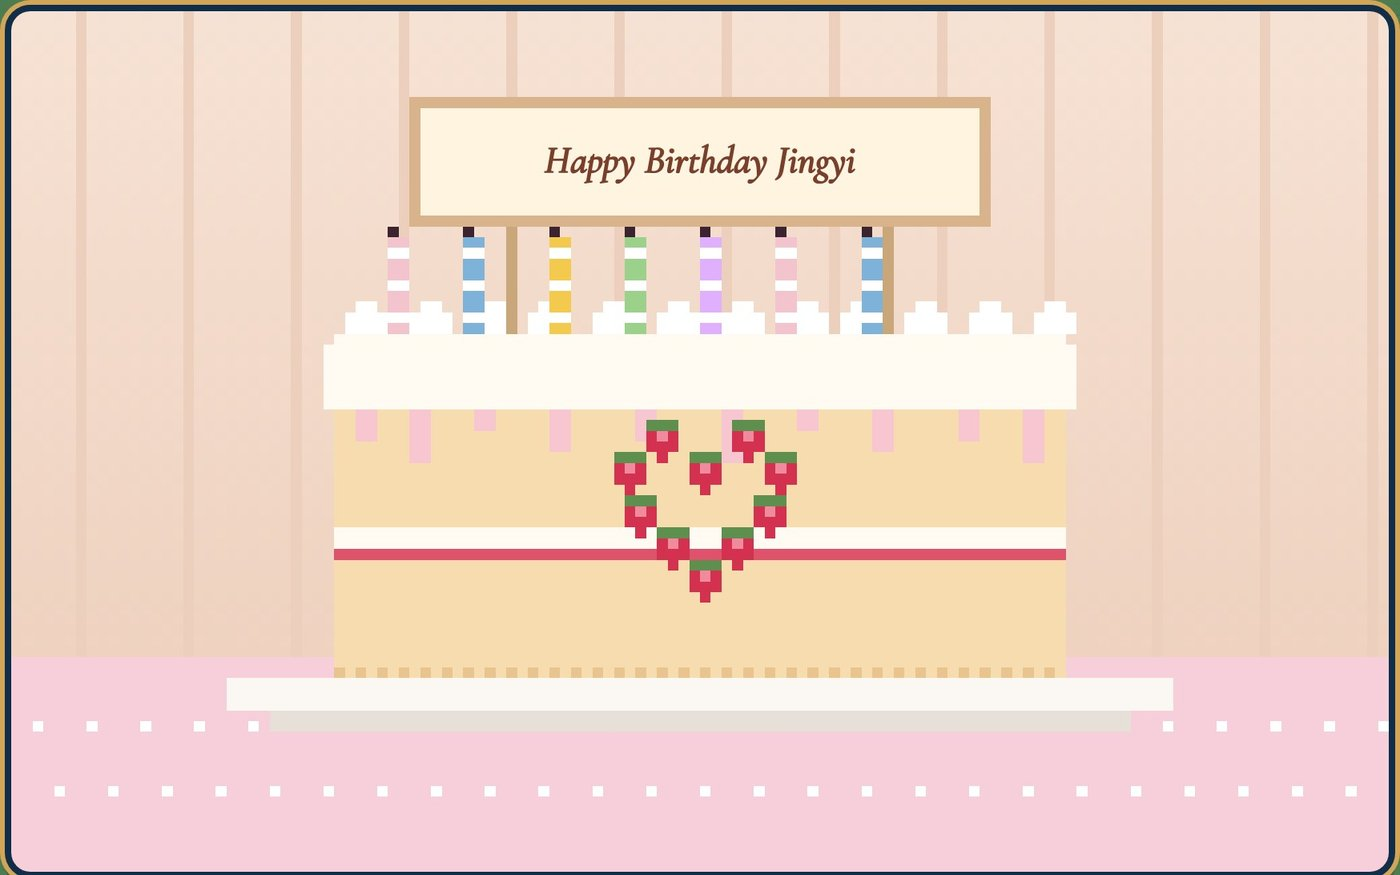
\includegraphics[width=0.245\textwidth]{figures/bday-27.jpg}\hfill
  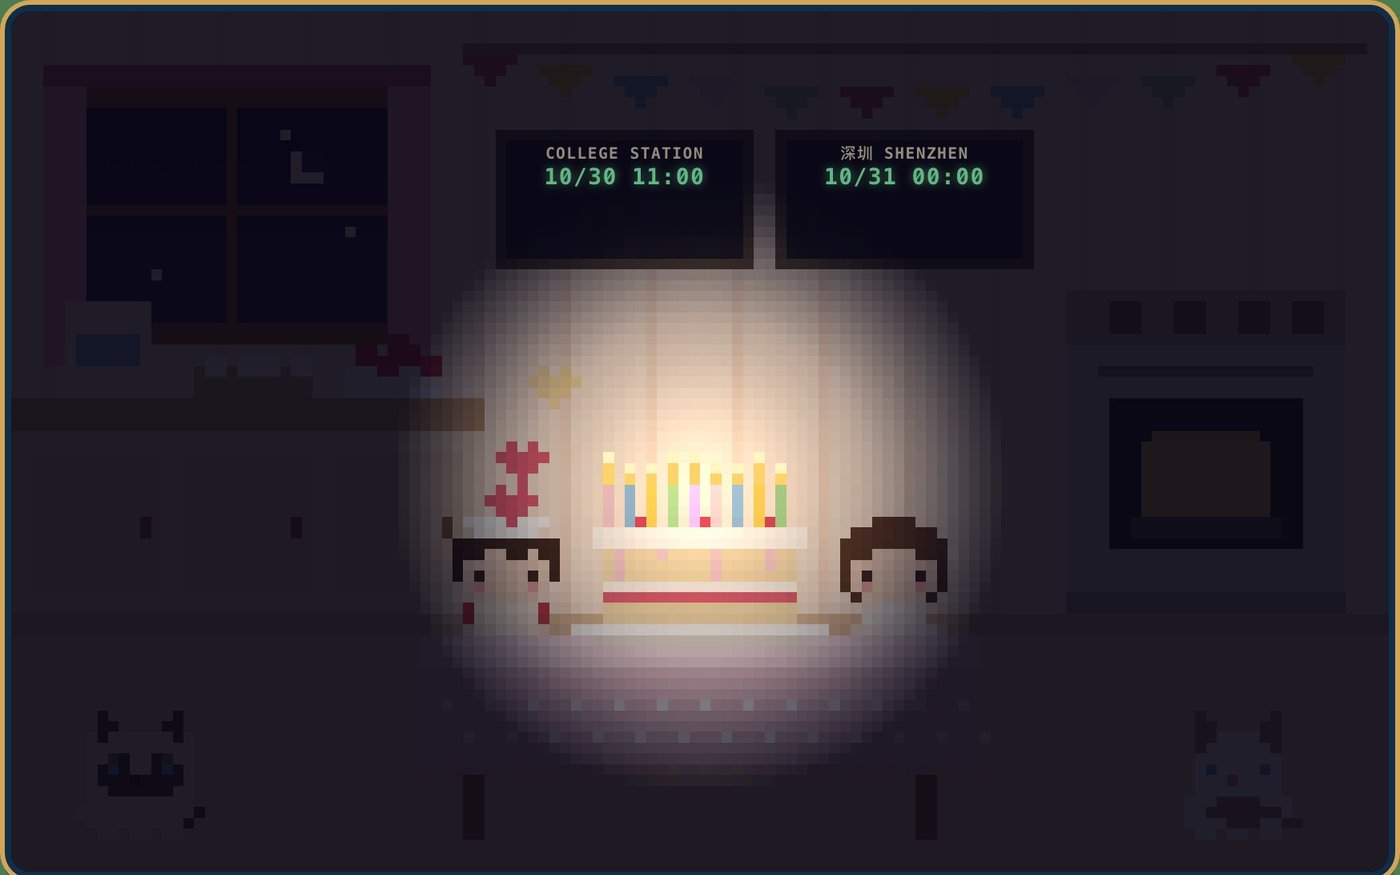
\includegraphics[width=0.245\textwidth]{figures/bday-37.jpg}\\[3pt]
  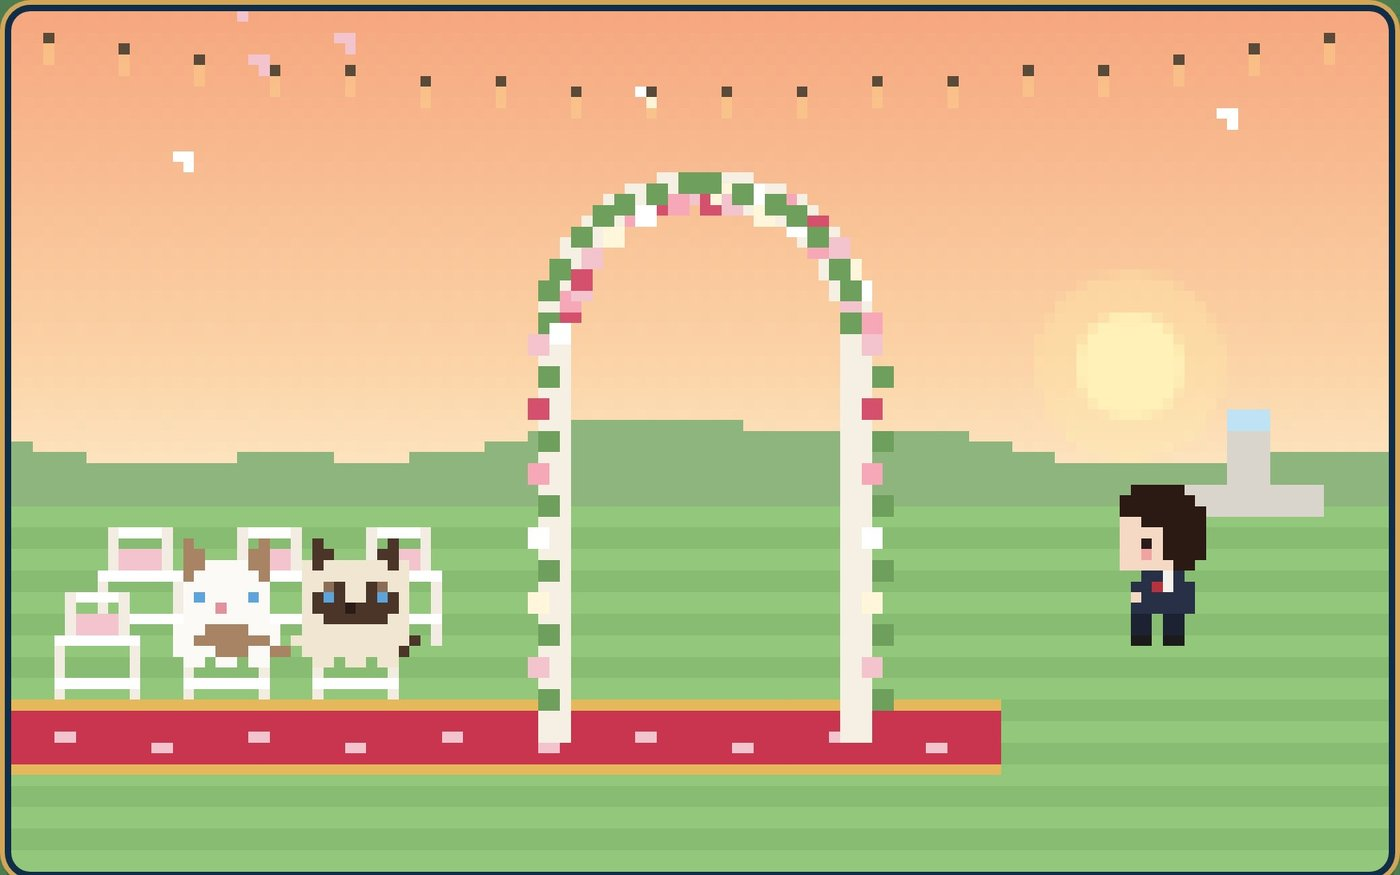
\includegraphics[width=0.245\textwidth]{figures/wed-03.jpg}\hfill
  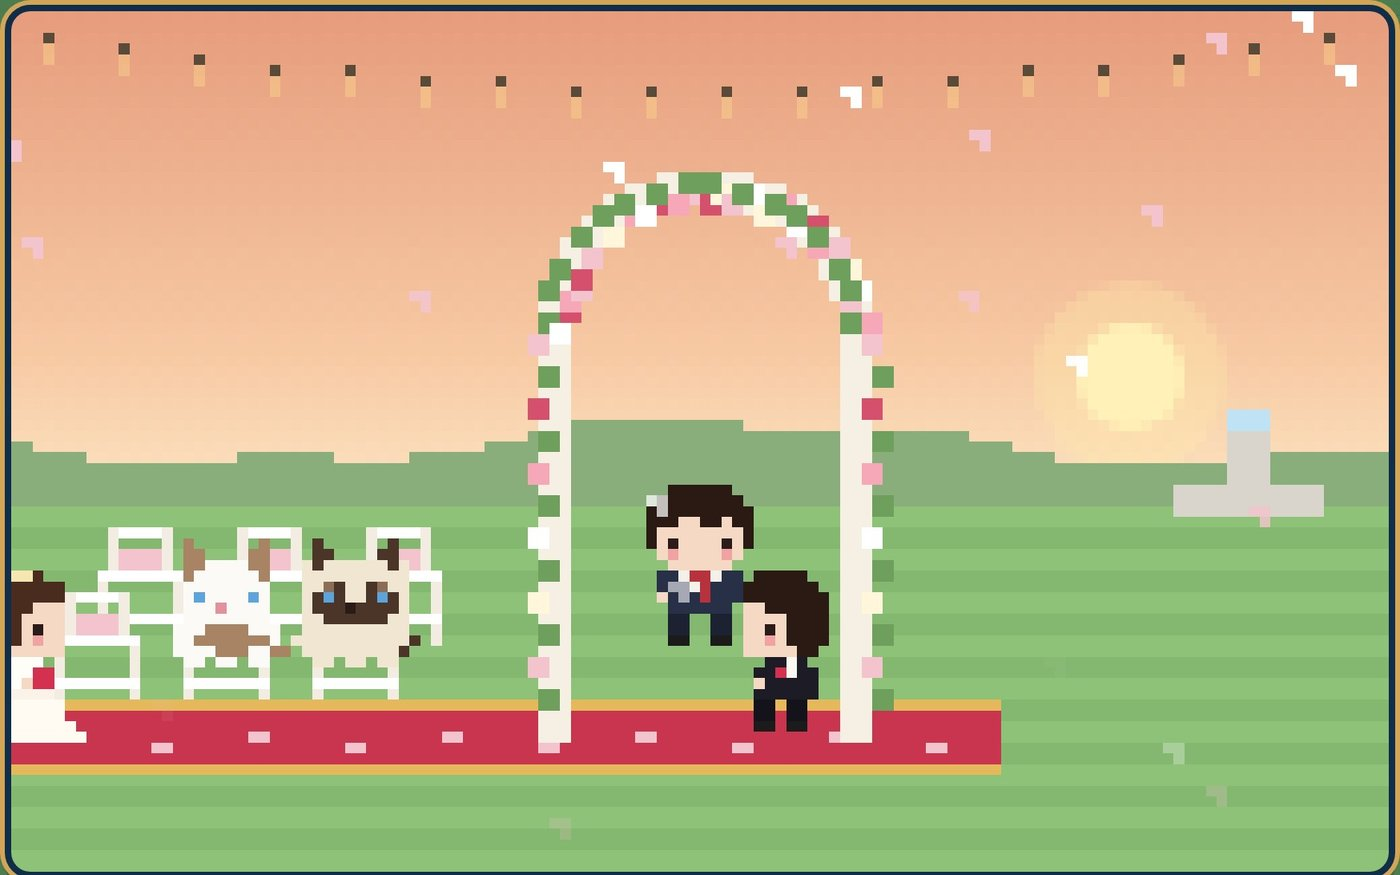
\includegraphics[width=0.245\textwidth]{figures/wed-11.jpg}\hfill
  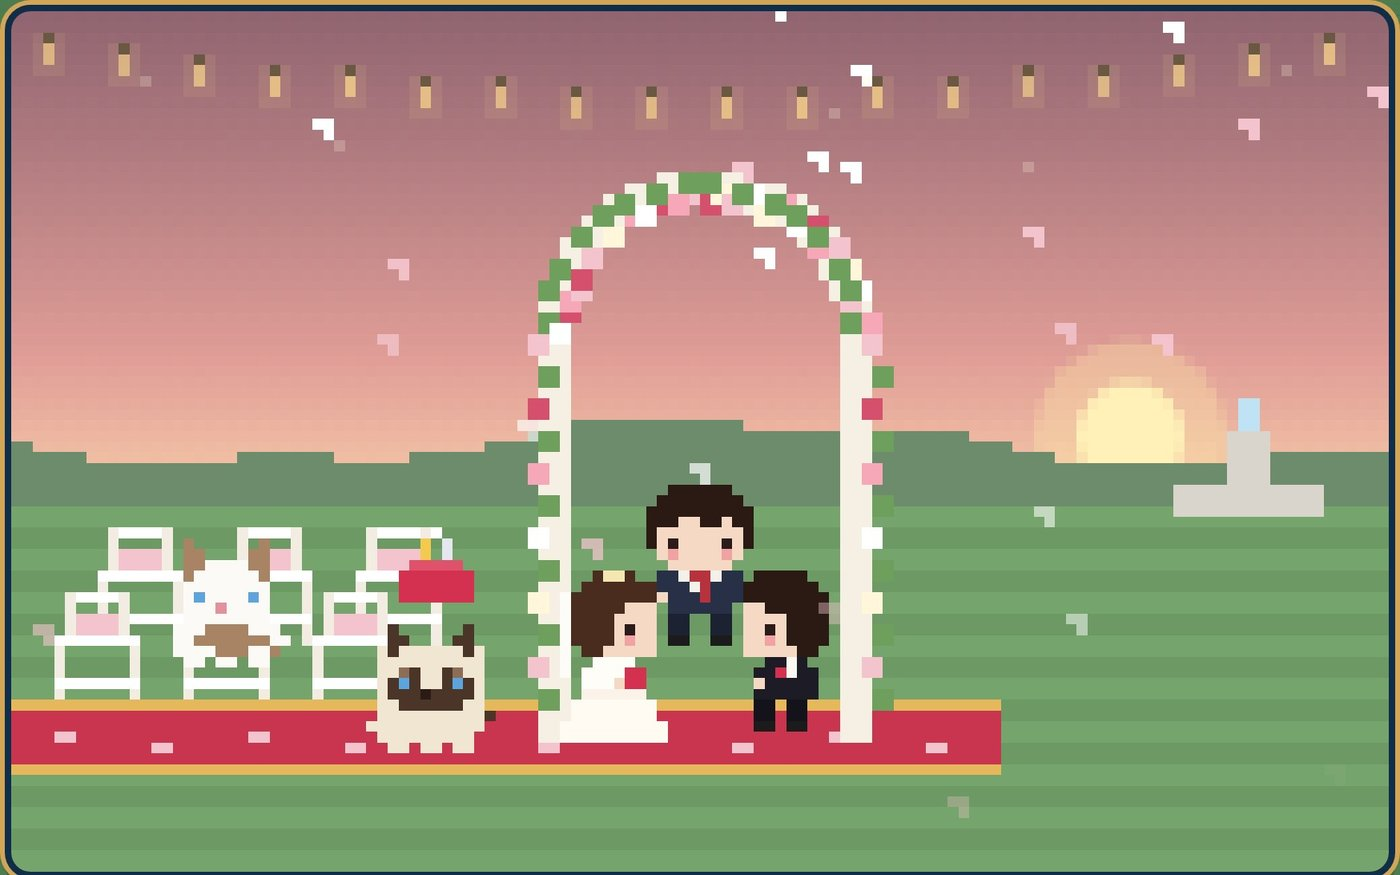
\includegraphics[width=0.245\textwidth]{figures/wed-21.jpg}\hfill
  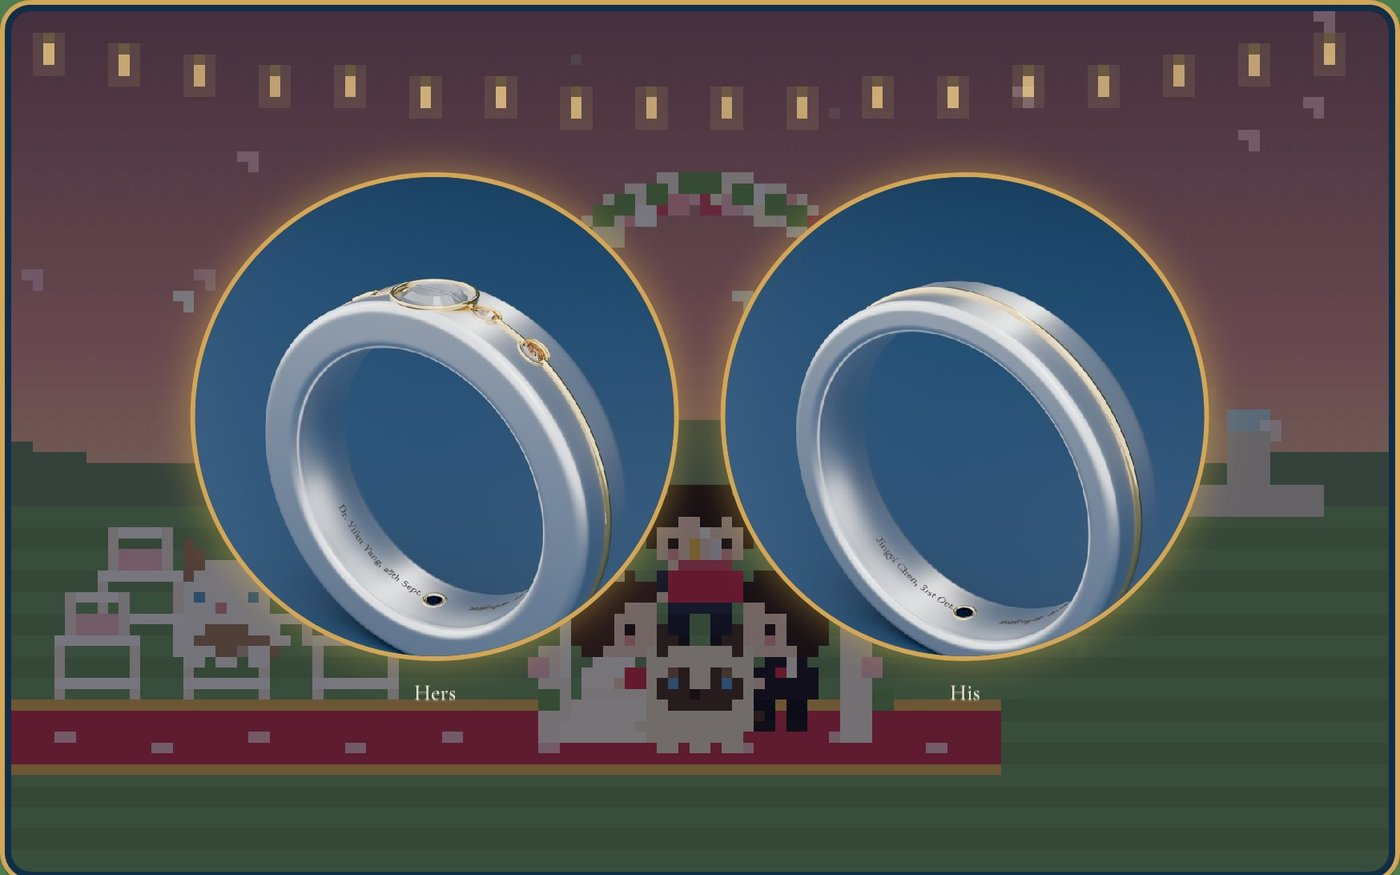
\includegraphics[width=0.245\textwidth]{figures/wed-23.jpg}
  \caption{The two cutscenes, left to right. Top, the birthday prologue: the kitchen at 9:47 a.m.\
  in College Station (10:47 p.m.\ in Shenzhen) with both clocks on the wall; whisking the batter;
  nine candles on the finished cake; singing at Shenzhen midnight with the cats. Bottom, the
  wedding: the guests take their seats; the bride walks the aisle; Coffee brings the rings; the
  Meridian rings in 3D over the ceremony.}
  \Description{Eight pixel-art frames. Top row: a pink kitchen, a chef at a table, a cake with
  candles, the same kitchen dark with candlelight. Bottom row: a garden with a flower arch at sunset,
  a couple under the arch, a cat carrying a pillow, two large 3D rings in circles.}
  \label{fig:cutscenes}
\end{figure*}

\begin{figure}[t]
  \centering
  
\includegraphics[width=0.78\columnwidth]{figures/wed-cert.jpg}
  \caption{The certificate at the end of the wedding, saved as an image through the phone's share
  sheet. It records the day of the ceremony, the day they met and the day they will meet.}
  \Description{A cream certificate card with two cartoon avatars and the names Yifan Yang and Jingyi Chen joined by a heart, on confetti.}
  \label{fig:cert}
\end{figure}

%% ===================================================================================
\section{System}\label{sec:system}

\subsection{Architecture}
\yt{} is a static single-page application in strict TypeScript, built with Vite and served from
static hosting under the couple's domain (Figure~\ref{fig:arch}). The deployment configuration
targets GitHub Pages. There is no author-operated backend for progress. Each feature
is a folder (\code{src/features/<name>/}) with its page module, styles, data, tests and a README,
and each page is a function \code{render(root) $\Rightarrow$ cleanup} loaded lazily by a path
router, so the main bundle carries only the shell and the town. Heavy modules (Leaflet for the map,
three.js for the ring, MediaPipe for the try-on) load only inside the level that needs them. A
service worker precaches the shell and caches eligible media after retrieval. The cached
town can run offline, but remote song embeds and browser-dependent speech recognition are not
guaranteed offline; cache eviction and previously unfetched assets also limit availability.

\begin{figure}[t]
  \centering
  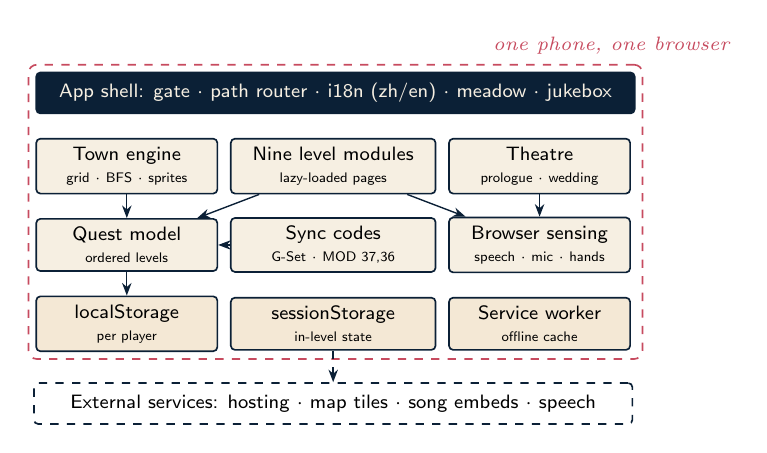
\begin{tikzpicture}[
      font=\scriptsize\sffamily,
      box/.style={draw=navy, line width=0.6pt, fill=cream, rounded corners=1.5pt, align=center, inner sep=3pt, minimum height=5.2mm},
      store/.style={box, fill=gold!25},
      ext/.style={box, dashed, fill=white},
      arr/.style={-{Stealth[length=1.6mm]}, navy, line width=0.5pt}]
    \node[box, minimum width=7.6cm, fill=navy, text=cream] (shell) {App shell: gate $\cdot$ path router $\cdot$ i18n (zh/en) $\cdot$ meadow $\cdot$ jukebox};
    \node[box, below=3mm of shell.south west, anchor=north west, minimum width=2.3cm] (town) {Town engine\\\tiny grid $\cdot$ BFS $\cdot$ sprites};
    \node[box, right=1.5mm of town, minimum width=2.6cm] (levels) {Nine level modules\\\tiny lazy-loaded pages};
    \node[box, right=1.5mm of levels, minimum width=2.3cm] (theatre) {Theatre\\\tiny prologue $\cdot$ wedding};
    \node[box, below=3mm of town, minimum width=2.3cm] (quest) {Quest model\\\tiny ordered levels};
    \node[box, right=1.5mm of quest, minimum width=2.6cm] (sync) {Sync codes\\\tiny G-Set $\cdot$ MOD 37,36};
    \node[box, right=1.5mm of sync, minimum width=2.3cm] (sense) {Browser sensing\\\tiny speech $\cdot$ mic $\cdot$ hands};
    \node[store, below=3mm of quest, minimum width=2.3cm] (ls) {localStorage\\\tiny per player};
    \node[store, right=1.5mm of ls, minimum width=2.6cm] (ss) {sessionStorage\\\tiny in-level state};
    \node[store, right=1.5mm of ss, minimum width=2.3cm] (sw) {Service worker\\\tiny offline cache};
    \node[ext, below=4mm of ss, minimum width=7.6cm] (ext) {External services: hosting $\cdot$ map tiles $\cdot$ song embeds $\cdot$ speech};
    \node[draw=rose, dashed, rounded corners=3pt, line width=0.6pt, fit=(shell)(ls)(sw), inner sep=2.5pt,
          label={[rose, font=\scriptsize\itshape]above right:one phone, one browser}] {};
    \draw[arr] (town) -- (quest); \draw[arr] (levels) -- (quest); \draw[arr] (levels) -- (sense);
    \draw[arr] (theatre) -- (sense); \draw[arr] (quest) -- (ls); \draw[arr] (sync) -- (quest);
    \draw[arr, dashed] (ss.south) -- (ext.north);
  \end{tikzpicture}
  \caption{Architecture of application modules and local state. The dashed boundary marks browser
  components, not a confidentiality boundary: static assets are hosted remotely, external requests
  expose request metadata, and speech recognition may use a remote service. Progress crosses
  devices through a manually exchanged code.}
  \Description{A block diagram: an app shell above three modules, which depend on a quest model,
  sync codes and browser sensing, which sit above three storage layers, all inside a dashed boundary
  labelled one phone, one browser; a dashed box below for external hosting, map, media and speech services.}
  \label{fig:arch}
\end{figure}

\subsection{The Quest Model}
Let $L = (\ell_1,\dots,\ell_9)$ be the ordered level registry and $C_p \subseteq L$ the set of
levels player $p$ has cleared on a device. A level is unlocked iff it is first or its predecessor
is cleared:
\begin{equation}
  \mathrm{unlocked}_p(\ell_i) \iff i = 1 \;\lor\; \ell_{i-1} \in C_p .
\end{equation}
Clearing adds to $C_p$ and nothing ever removes from it, except an explicit reset. The router
enforces the lock, and a second guard requires that a level be entered through its door: walking
onto the door sets a one-shot token in \code{sessionStorage}, and a level route without the token
redirects to the town. Level numbers are derived from the registry, so inserting a level (the
Poems level was inserted before the last one during development) renumbers every house, sign and
string at once; a test fails until the new house has a door that the town's path search can reach.

\subsection{Progress without a Server}
Each phone holds its own $C_p$. Because $C_p$ only grows, it is a grow-only set (G-Set), the
simplest state-based CRDT~\cite{shapiro2011crdt}: the merge of two replicas is their union,
\begin{equation}
  C_p \sqcup C'_p = C_p \cup C'_p ,
\end{equation}
which is commutative, associative and idempotent. Replicas converge if all updates are eventually exchanged, both phones use the same
level registry and no reset occurs. Repeated imports are idempotent; an old code cannot remove
completion flags, but incomplete exchange can leave the two views different. The
only channel needed is one the couple already use every day: a chat message.

\paragraph{Progress codes.} A code encodes one player and a bitmask of cleared levels,
$m = \sum_{\ell_i \in C_p} 2^{\,i-1}$, written in base 36 after a player letter (\code{J} or
\code{Y}) and followed by one check character. With nine levels $m \le 511 = \mathrm{E7}_{36}$, so a
code is at most four characters: \code{JVA} says that Jingyi has cleared $m = 31$, the first five
levels (Table~\ref{tab:codes}). The check character follows the hybrid system ISO~7064
MOD~37,36~\cite{iso7064}. Writing $a_j \in \{0,\dots,35\}$ for the value of the $j$-th body
character and starting from $p_0 = 36$,
\begin{equation}
  s_j = \big((p_{j-1} + a_j) \bmod 36\big) \text{ or } 36 \text{ if } 0, \qquad
  p_j = 2 s_j \bmod 37 ,
\end{equation}
and the check character is the symbol of value $(37 - p_n) \bmod 36$. We checked the scheme exhaustively over all
1{,}024 valid codes. It rejects every one of the codes' single-character substitutions. Of the
2{,}943 transpositions of two different adjacent characters, it rejects all but five. One of
those (\code{JI0}$\to$\code{IJ0}) is still refused because \code{I} is not a player letter. The
other four all swap a \code{0} and a \code{1} inside the mask (\code{J801}$\leftrightarrow$\code{J810},
\code{YE01}$\leftrightarrow$\code{YE10}): the rule above maps a running sum of 0 to 36, so a zero
digit and its neighbour can trade places unseen. The exhaustive check covers 140{,}840 substitutions and 2{,}943 unequal adjacent swaps
of canonical codes; the decoder rejects all substitutions and accepts four directed swaps
(two bidirectional pairs). This is an error-detection check, not a user transcription study.
An accepted typo may add unearned completion flags and unlock later content, including the finale. An earlier version used a plain weighted sum,
which let some one-character typos through; it was replaced during a review pass, invalidating older
codes. Codes are not authenticated: a person can construct completion for either player. They
carry no schema version, so registry insertions or reordering can reinterpret bits. Reset is outside
the grow-only model; importing an earlier code after reset restores its flags. A code may also
travel in a link (\code{/sync?c=JVA}), exposing its payload to the hosting request and potentially
to browser history or the channel through which it is sent.

\begin{table}[t]
  \caption{Example progress codes: player letter, base-36 mask and the check character of Eq.~3.}
  \label{tab:codes}
  \small
  \begin{tabular}{@{}lrll@{}}
    \toprule
    Cleared & Mask $m$ & Base 36 & Code \\
    \midrule
    Jingyi, levels 1--5 & 31 & \code{V} & \code{JVA} \\
    Jingyi, all nine & 511 & \code{E7} & \code{JE7Z} \\
    Yifan, all nine & 511 & \code{E7} & \code{YE7O} \\
    Yifan, none & 0 & \code{0} & \code{Y0C} \\
    \bottomrule
  \end{tabular}

\end{table}

\paragraph{Three layers of storage.} Cleared levels live in \code{localStorage} under a key per
player; half-finished state inside a level (the Gomoku position reached, the stars joined so far)
lives in \code{sessionStorage}, so a reload or a language switch inside a level does not restart it,
and it is dropped when the level is cleared; and a service worker keeps the site itself. When the
browser blocks storage, an in-memory store keeps progress for the visit.

\subsection{The Town Engine}
The town is a grid of characters (\code{.}\ grass, \code{\#} path, \code{\textasciitilde}\ water,
\code{T} tree, \code{O} fountain, and so on). Movement is one tile per 190\,ms with an ease-out
interpolation; the pure functions \code{step} and \code{faced} decide movement and facing and are
unit-tested, while a class wires them to a canvas and one animation loop. A tap on the map runs a
breadth-first search over walkable tiles and queues the resulting steps. The camera follows the
player. The same engine takes any map, so the two cities reuse it with their own grids, roads and a
basketball court.

\paragraph{Art as text (\dc{5}).} A sprite is an array of strings, one character per pixel, and
a palette that maps characters to colours. A figure is a $12\times12$ body per facing over four
rows of legs shared between facings, so a walk cycle is the same two leg frames under different
bodies, and the side view is mirrored. Tiles (grass with flowers, paths that join their neighbours,
roofs in each level's colour, lit windows) are painted procedurally. The README banner, the favicon
and the app icons are generated from the same strings by scripts, so a new outfit appears
everywhere at once.

\paragraph{Daylight by city.} Let $h_p$ be the current hour in player $p$'s time zone
(\code{Asia/Shanghai} or \code{America/Chicago}). The phase is dawn for $h_p \in [6,7)$, day for
$[7,17)$, dusk for $[17,19)$ and night otherwise; dawn, dusk and night each lay a coloured wash over
the map (night: navy at 42\% opacity) and light the windows. In the two cities the person's
position is $\mathrm{stopAt}(h) = $ the first stop whose hour windows contain $h \bmod 24$.

\subsection{Sensing in the Browser}\label{sec:sensing}
Camera tracking and breath-amplitude processing run in application code on the device.
Browser speech recognition has a different processing boundary.

\emph{Voice.} The vow and the wedding's ``I do'' use the Web Speech API~\cite{w3c2023speech} in
Mandarin. The implementation does not require on-device recognition; the API allows a
remote recognition service unless local processing is explicitly required~\cite{w3c2023speech}.
The application therefore cannot guarantee that voice samples remain on-device. A typed fallback
is available for the vow. Recognition alternatives are normalised to Han characters and Latin
letters; the matcher accepts a phrase when it contains \zh{我爱你}, \zh{我愿意} and any accepted spelling of the
partner's name.

\emph{Breath.} Blowing out the candles reads the microphone with echo cancellation, noise
suppression and gain control off, computes the root-mean-square loudness of each 1{,}024-sample
frame, smooths it ($s \leftarrow 0.6s + 0.4\min(1, 5\,\mathrm{rms})$), and blows when $s > 0.32$.
We rely on a breath being a loud, broadband rush on a phone microphone; the threshold was set by
hand and has not yet been calibrated across devices.

\emph{Hands.} The try-on runs MediaPipe's hand landmarker~\cite{lugaresi2019mediapipe,zhang2020hands}
on the camera stream. The ring sits on the ring finger's proximal phalanx, 38\% of the way from
landmark 13 (the knuckle) to landmark 14; its axis follows the finger, and its ``up'' is the back of
the hand, from the palm normal and the reported handedness. Scale comes from anatomy: the mean
spacing of the middle, ring and little knuckles serves as the ruler, set to a constant of 19.5\,mm
(our working estimate for an adult hand, not a measured value), so
\begin{equation}
  \text{px/mm} = \tfrac{1}{2}\,\big(\lVert k_9 - k_{13}\rVert + \lVert k_{13} - k_{17}\rVert\big) \,/\, 19.5 ,
\end{equation}
and nominal model dimensions map to the screen under this assumed scale. The display
is a stylised overlay, not a validated measurement of ring size or fit. Position, rotation and scale are
smoothed (factor 0.45 per frame). The shutter composes the photo with a caption, and a second card
puts both players' try-on photos side by side.

\subsection{Keeping a Secret with a Test (\dc{6})}
The ring is the surprise at the end, and an interface that hints at it spoils it. Rayford, the
town, the progress page and the cats all speak before the ring is reached, and their lines were
written and rewritten over days. Rather than rely on vigilance, a unit test scans every key in
the bilingual dictionary, except the keys shown only after the ring, and fails if any contains
\zh{戒} (ring) in Chinese, \emph{ring} as a word in English, or any word for wedding, marriage,
proposal, bride or groom in either language. One exception is listed by name: Jingyi's own joke on
the Shenzhen Bay stop, which is about a flat, not a ring. The test establishes absence of specified lexical patterns in the selected dictionary
entries. It does not inspect all assets, routes, source code or indirect visual cues, and therefore
does not establish secrecy against inspection or unexpected navigation.


\subsection{Implementation and Verification}
Table~\ref{tab:metrics} describes the version 1.17.0 implementation. A revision audit reran the
existing suite: all 153 tests in 36 files passed, and the strict TypeScript check and production
build succeeded. The main JavaScript chunk was 114.09\,kB (42.58\,kB gzip), and the service worker
precached 44 entries totalling 302.12\,KiB. Bundle sizes describe this build environment, not
measured load time on users' phones. The large ring, map and try-on chunks are lazy loaded.

The audit also independently enumerated the progress-code cases reported above. Dictionary tests
check matching non-empty keys; puzzle tests check properties such as unique winning moves.
Passing these tests supports their asserted properties, not overall usability, privacy or an
effect on intimacy. For example, the suite passes with 21 stars even though the earlier manuscript
reported 22, because its star tests check consistency rather than that prose count.

The development records describe browser checks at desktop, 390-pixel and 320-pixel widths and a
laptop-camera check of hand orientation. The inspected repository does not contain an archived
per-release end-to-end report supporting the earlier claim that every release completed all nine
levels at every stated width in both languages. That stronger claim is not retained. Systematic
phone checks of speech, breath, camera completion and sharing remain outstanding, as does any
recipient or relationship evaluation.

\begin{table}[t]
  \caption{Implementation summary (version 1.17.0, 28 October 2026).}
  \label{tab:metrics}
  \small
  \begin{tabular}{@{}p{0.56\columnwidth}p{0.36\columnwidth}@{}}
    \toprule
    Measure & Value \\
    \midrule
    TypeScript source, excluding tests (lines) & 8{,}414 \\
    CSS (lines) & 1{,}080 \\
    Bilingual dictionary (lines) & 791 \\
    Test files / unit tests & 36 / 153 \\
    Commits / versions (24--28 Oct.\ 2026) & 109 / 28 \\
    Main bundle (min.\ / gzip) & 114\,kB / 43\,kB \\
    Precached shell (service worker) & 44 files, 302\,KiB \\
    Feature folders & 24 \\
    Runtime dependencies & 3 (Leaflet, three.js, MediaPipe) \\
    Author-operated progress backend / app accounts & 0 / 0 \\
    \bottomrule
  \end{tabular}
\end{table}

%% ===================================================================================

\section{Reconstructing Design Decisions}\label{sec:log}
Four documented episodes make the rationale inspectable. Commit identifiers distinguish recorded
changes from our interpretations; neither a diff nor its message establishes a user outcome.

\paragraph{Replacing Pictionary (\code{7d2c659}, 26 October).}
The implementation removes a same-device drawing game and adds a song-identification level.
Our interpretation is that separate recognition of a shared song better accommodates different
visit times than taking turns on one screen. The diff establishes the replacement, not that
the recipient preferred songs or that music increased closeness. A different reading is simply
that the replacement reduced implementation complexity.

\paragraph{Requiring a try-on photo (\code{2bc3d07}, 28 October).}
The ring level's completion condition changes from viewing the reveal to capturing a try-on
photo. This creates an artefact that can be shared, but also makes camera access and a capable
device conditions for completing the narrative. The same mechanism can be read as participation
or as an unwanted demand. No recipient account resolves that tension here.

\paragraph{Correcting represented routines (\code{1960404}, 26 October).}
The city-day descriptions change the transport and destination details to match the designer's
account of the couple's routines. The record shows that plausible generated defaults required
correction. It does not independently validate the representation of the other partner. Personal
recognition is the design intention; verification by the represented person is still needed.

\paragraph{Revising the entry gate (\code{ccabd31}, 28 October).}
The review removes answer-revealing placeholder text and revises associated checks. This makes
the recognition question less self-defeating, but does not turn a low-entropy, client-side date
gate into access control. Its social role and its security properties must be evaluated separately.

Across these episodes, the transferable issue is how a technical rule expresses an assumption
about the other person. The records support the existence of those assumptions and revisions;
their acceptance, emotional meaning and durability require different evidence.

%% ===================================================================================

\section{Discussion}\label{sec:discussion}


\subsection{From Representation to Action}
The design links a shared reference to an action, then to a visible trace: a prior game becomes
a win-in-one puzzle and its solution becomes one point of a heart. Compared with displaying the
same memory as a caption, this adds an authored sequence of participation. The proposed design
opportunity is to examine which part of a memory can become a rule without losing its meaning.
The case demonstrates a concrete implementation of that move, not that it is more effective
than a photo album, a message or another intimate artefact~\cite{hassenzahl2012love,kirk2016ritual}.
The ring also exposes a boundary: an imagined future is not a remembered event, although both
can organise narrative play.

\subsection{Privacy Boundaries and Personal Material}\label{sec:privacy}
The gate hashes a low-entropy date, whose value may also be inferred from the surrounding story.
It deters casual entry but provides neither encryption nor dependable access control. Local
completion flags avoid an author-operated progress database; they do not make hosted photographs,
voice notes or letters private. The voice-note implementation, for example, references a static
audio asset. Anyone authorised to obtain the deployed files or repository may obtain such material.

The browser boundary also differs by feature. Hand tracking and breath-amplitude calculation
run locally, whereas speech recognition may contact a remote service. Tile and media requests
expose request metadata to their providers. A local-first aspiration therefore needs a description
of data flows, not only the absence of a custom backend~\cite{kleppmann2019localfirst}.
An appropriate public research release would separate shareable code and synthetic examples
from personal assets; intimate images can also reveal location context~\cite{yang2024geolocator}.
That separation is a release task, not a property established by the current artefact.

\subsection{Asynchrony, Temporal Representation and Staleness}
Each player's sky uses the clock in their configured city, while the partner avatar represents
locally stored progress. The design supports visiting at different times, but an avatar's state
may be old until the next manual exchange. Its city-day position follows an authored schedule,
not sensed presence. This distinction matters: a representation intended as companionship can
otherwise imply knowledge of the partner's current activity that the system does not have.
The birthday scene's scripted clocks and the variable thirteen- or fourteen-hour offset are
temporal design materials~\cite{hallnas2001slow,odom2012technology}, not evidence of temporal
co-presence or synchronised participation.

\subsection{Staged Access, Surprise and Freedom to Decline}
Ordered access and delayed disclosure coordinate a surprise, but also let one partner determine
what the other must do before reaching a letter or finale. Requiring a photograph illustrates the
cost: people without camera access, or who prefer not to provide an image, cannot clear that level
through the current completion rule. Similarly, a scripted ``I do'' is a game response, not evidence
of consent to a relationship commitment. The present sequence does not model refusal as a separate
successful outcome. A future revision should distinguish declining an action from failing a task
and should offer an equivalent path that preserves narrative access.

The lexical test is useful as a writing regression check, but it cannot ensure surprise in a
client-delivered game. Source, routes, media, screenshots and this paper disclose the finale.
Any study of surprise must therefore record whether the recipient encountered these materials
before play. Ambiguity may shape anticipation~\cite{gaver2003ambiguity}; this case does not yet
establish how it was experienced.

\subsection{Bilingual Coverage and Situated Meaning}
The same-key test prevents missing dictionary entries, but does not establish equivalent meaning,
tone or task difficulty. The Chinese title \zh{仪见钟情} substitutes a character from Jingyi's name
into ``love at first sight''; the English version explains the reference. Likewise, classical
Chinese character-restoration puzzles retain different language demands even when their prompts
have English versions. A defensible claim is coverage of intended interface strings in two
languages. Semantic quality and the accessibility of the resulting experience require a separate
review, including by the intended recipient.

\subsection{AI Assistance and Authorial Responsibility}
The source and log document an AI-assisted implementation process in which the designer supplied
requirements and corrected defaults. A correction shows a disagreement with generated output;
it does not establish that all other generated details were accurate. The contribution is therefore
the inspectable artefact and the rationale for selected choices, rather than a productivity claim
inferred from five days of work. The corpus lacks an unassisted comparison and a complete record
of human and model effort. Personal representation, verification and publication decisions remain
the authors' responsibilities.

\subsection{Limitations and Next Evidence}
The principal limitation is evidential: developer playtesting is the only reported use, and no
recipient experience, sustained practice or relationship outcome has been collected. The corpus
is brief and selectively interpreted, with no independent analysis. Engineering checks are also
bounded: tests do not establish deployment-wide privacy, all-browser compatibility or equivalent
experience across languages; approximate hand scaling is not a fit measurement. Union merge
depends on compatible registries and does not propagate resets. Remote media limits offline use
and availability across regions.

A next stage could begin with a voluntary recipient walkthrough, recording what was understood,
skipped, refused or reinterpreted, followed by a diary of revisits and code exchanges over time.
These are proposed studies, not completed work. If participants are recruited or data are collected
under an institution, the applicable ethics determination must precede that collection. A larger
sample alone would not repair missing accounts of situated meaning, authorial power or failure.

%% ===================================================================================


\section{Conclusion}
MERIDIAN documents the pre-deployment design of a two-person game that turns autobiographical
material into tasks, places and staged ceremonies. Its development record makes four design
revisions inspectable, and its implementation audit establishes selected software properties.
These support a situated account of how memories can shape playable rules. They do not establish
that the game improves intimacy or that the recipient accepts its authored sequence. The central
open question is how a personal gift can invite shared meaning while leaving the other person
free to decline, reinterpret and reshape it.

\section*{Ethics and Publication Scope}
This manuscript reports design and implementation, without recipient interviews or a relationship
evaluation. Authorship, participation in play and permission to disclose personal material are
separate decisions. Publication of identifiable narratives, dates, images, voices or represented
routines requires the agreement of the people concerned; being a co-author is not a substitute
for approving each category of disclosure. The manuscript does not report an institutional ethics
approval or exemption. Any future study requires an appropriate determination before data collection.

\section*{Code and Data Availability}
The inspected implementation is version 1.17.0 at commit \code{55440ae}; manuscript revision began
from \code{94ce914}. The repository is located at \url{https://github.com/rayford295/yi-town}
and was private when checked on 29 October 2026. A separately released, privacy-reviewed code
archive and persistent archive identifier are not yet available. Personal photographs, voice
notes and letters are not offered as a public research dataset. Repository visibility and consent
must be rechecked when preparing any public release; the current statement does not promise
unrestricted access to personal assets.

\section*{Declaration of Generative AI Use}
The original manuscript reports use of Claude (Anthropic) through Claude Code for much of the
software implementation, manuscript drafting and figure preparation. This revision additionally
used Codex (OpenAI) for source inspection, editorial suggestions and implementation checks.
Automated assistance and bibliographic metadata checks do not establish the truth of personal
accounts or replace author review. The authors remain responsible for verifying the manuscript,
attributions, reported evidence and permissions before submission. No AI system is listed as an author.

\begin{acks}
To Coffee and Duoduo, who guard the doors. The street-view photographs on the Love Map are from
Wikimedia Commons and credited in the game; the \emph{Wedding March} is a public-domain recording
from the European Archive.
\end{acks}

\bibliographystyle{ACM-Reference-Format}
\bibliography{references}

\end{document}
